\subsection{Przebiegi -- Scenariusz S1 (nominalny)}
\begin{figure}[p]\centering
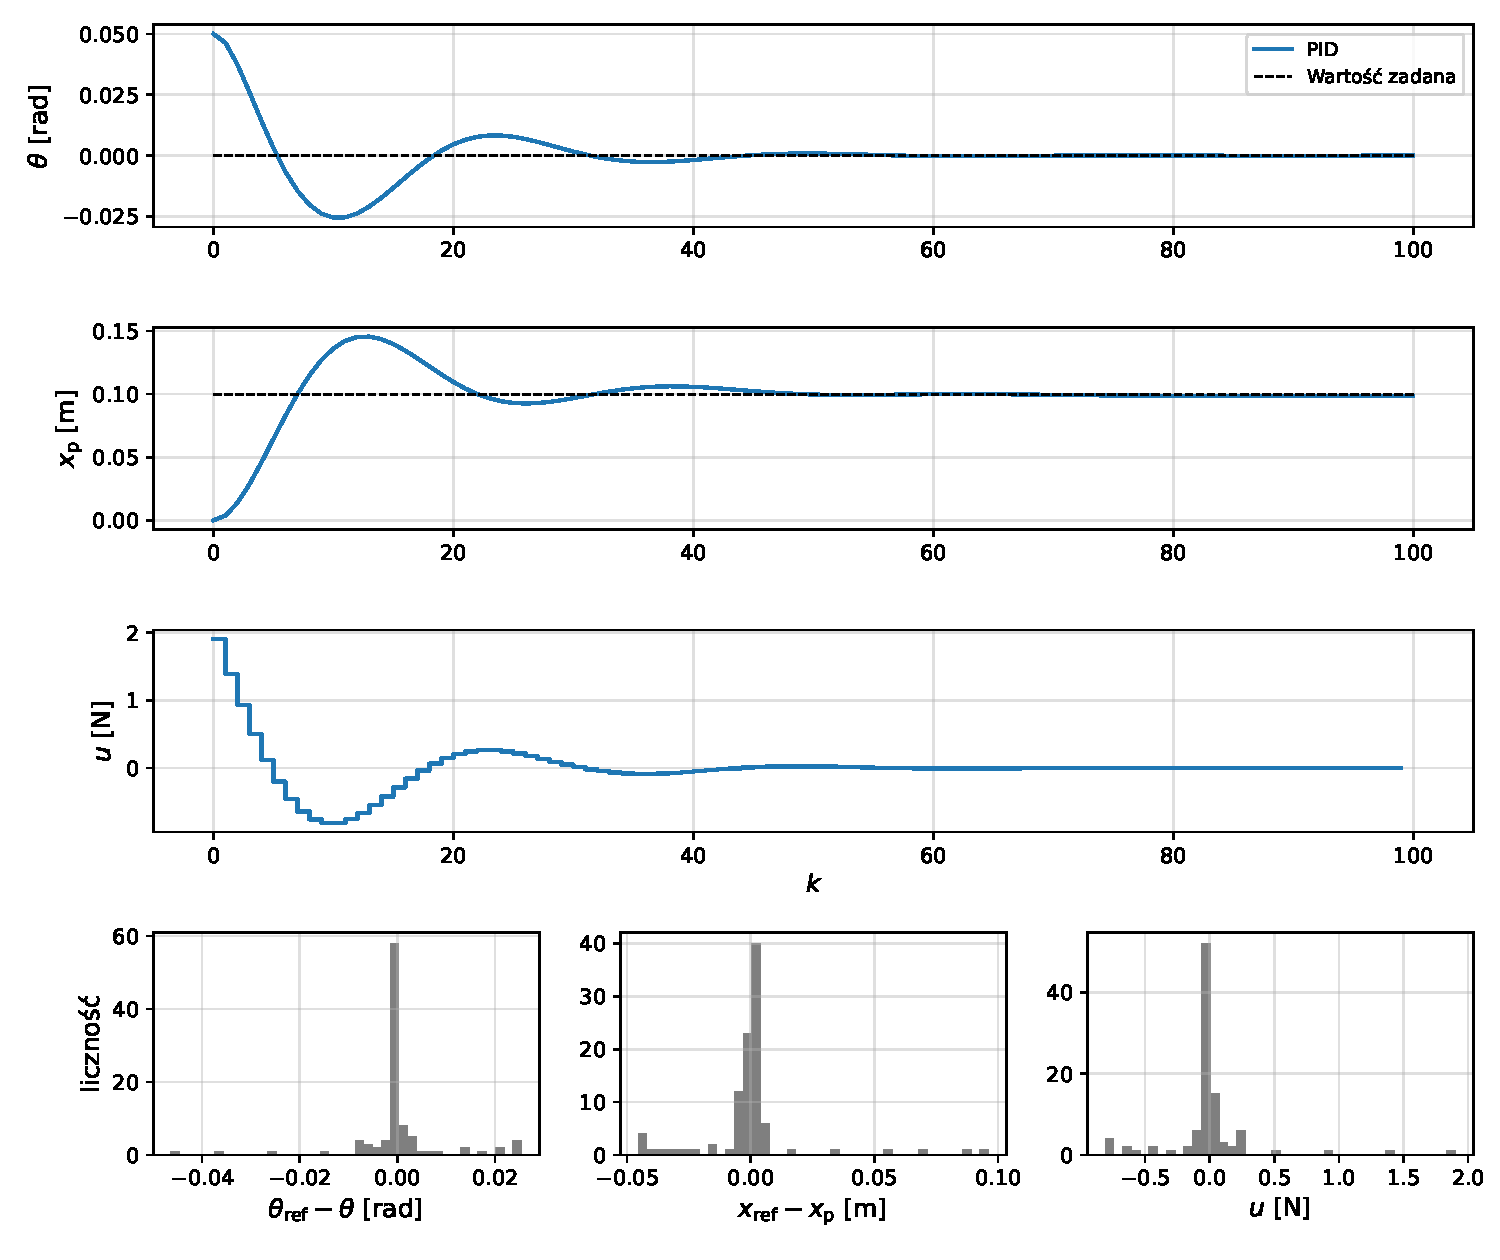
\includegraphics[width=\linewidth]{figs/S1_pid.pdf}
\caption{PID, Scenariusz S1 (nominalny): status automatyczny -- stabilny.}
\end{figure}
\clearpage
\begin{figure}[p]\centering
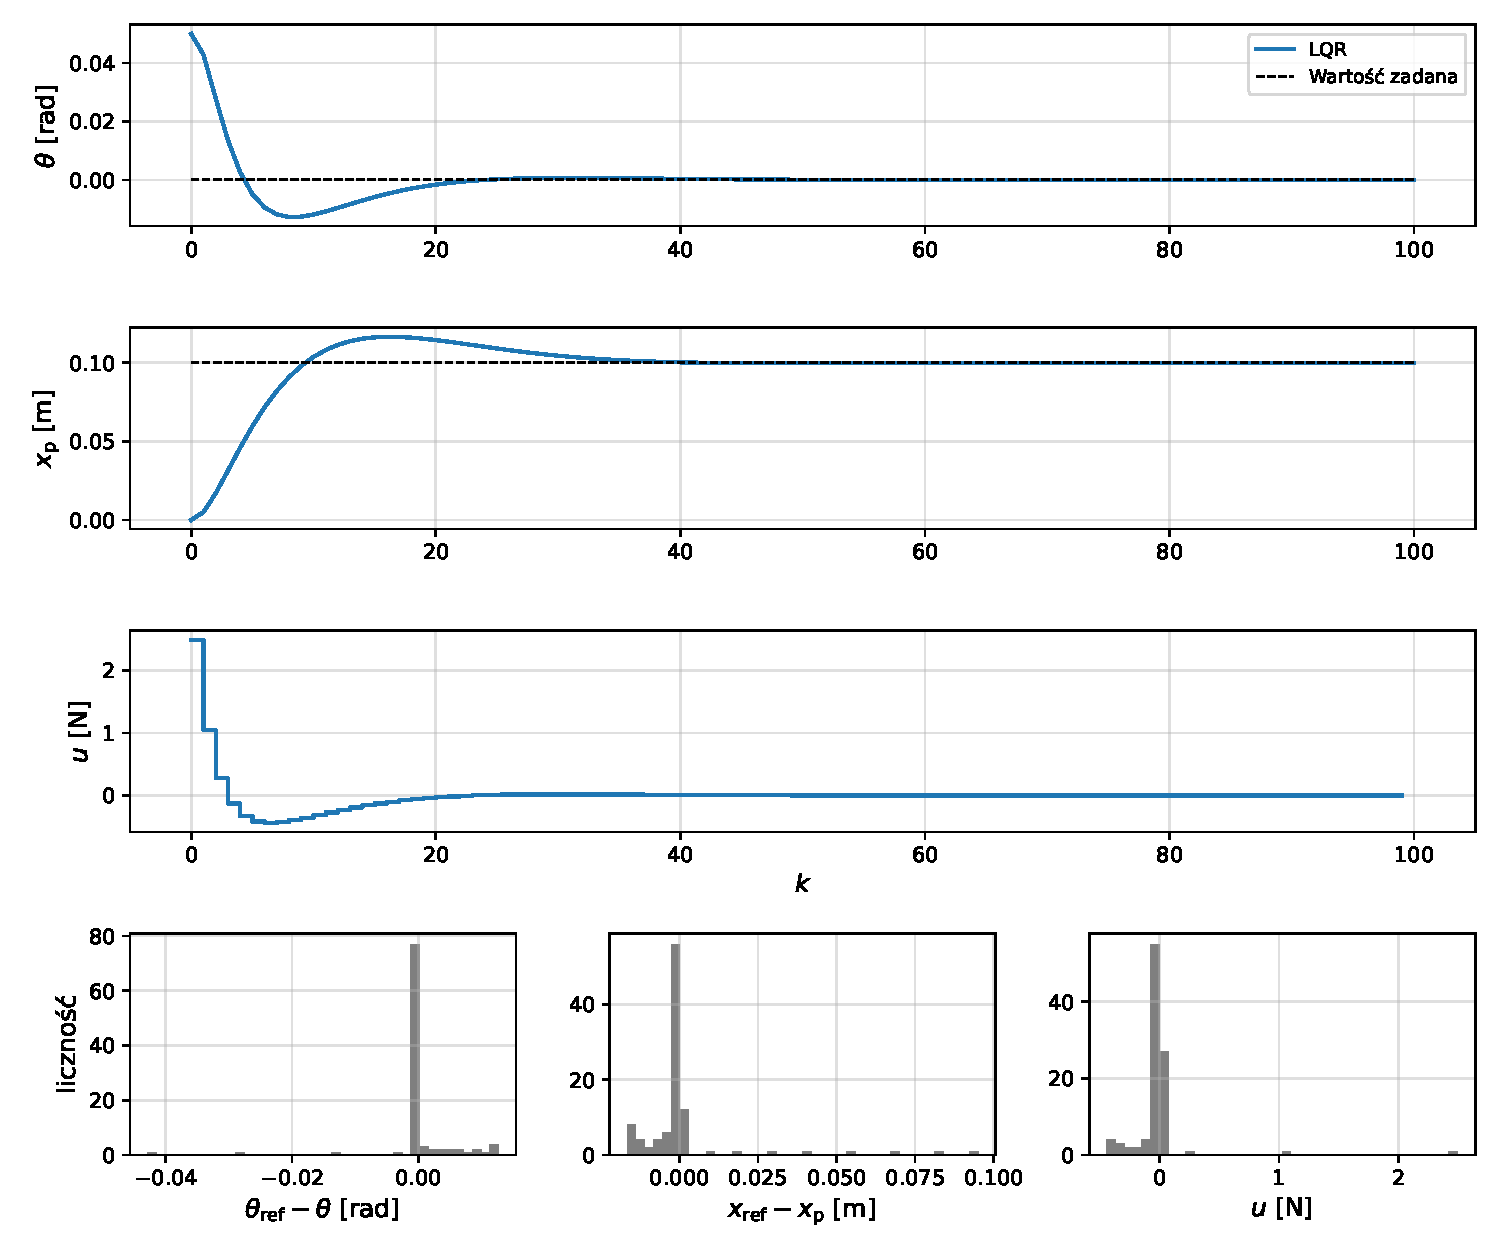
\includegraphics[width=\linewidth]{figs/S1_lqr.pdf}
\caption{LQR, Scenariusz S1 (nominalny): status automatyczny -- stabilny.}
\end{figure}
\clearpage
\begin{figure}[p]\centering
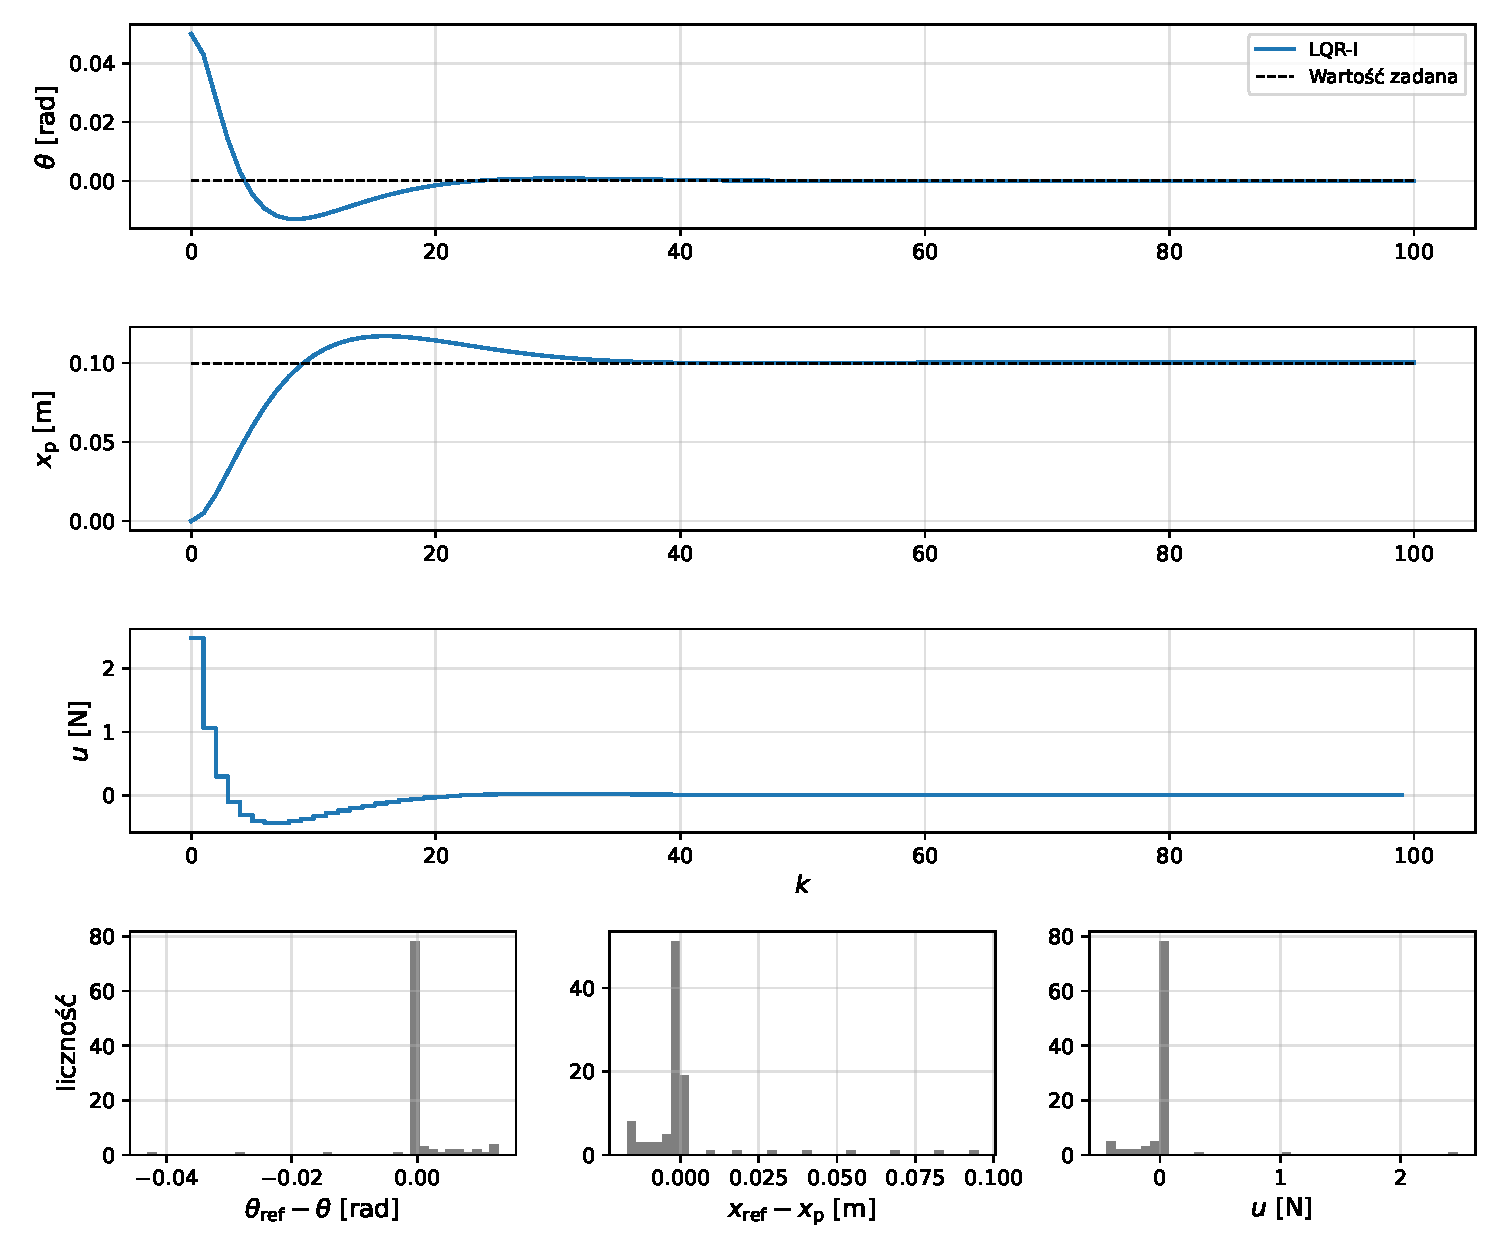
\includegraphics[width=\linewidth]{figs/S1_lqr_i.pdf}
\caption{LQR-I, Scenariusz S1 (nominalny): status automatyczny -- stabilny.}
\end{figure}
\clearpage
\begin{figure}[p]\centering
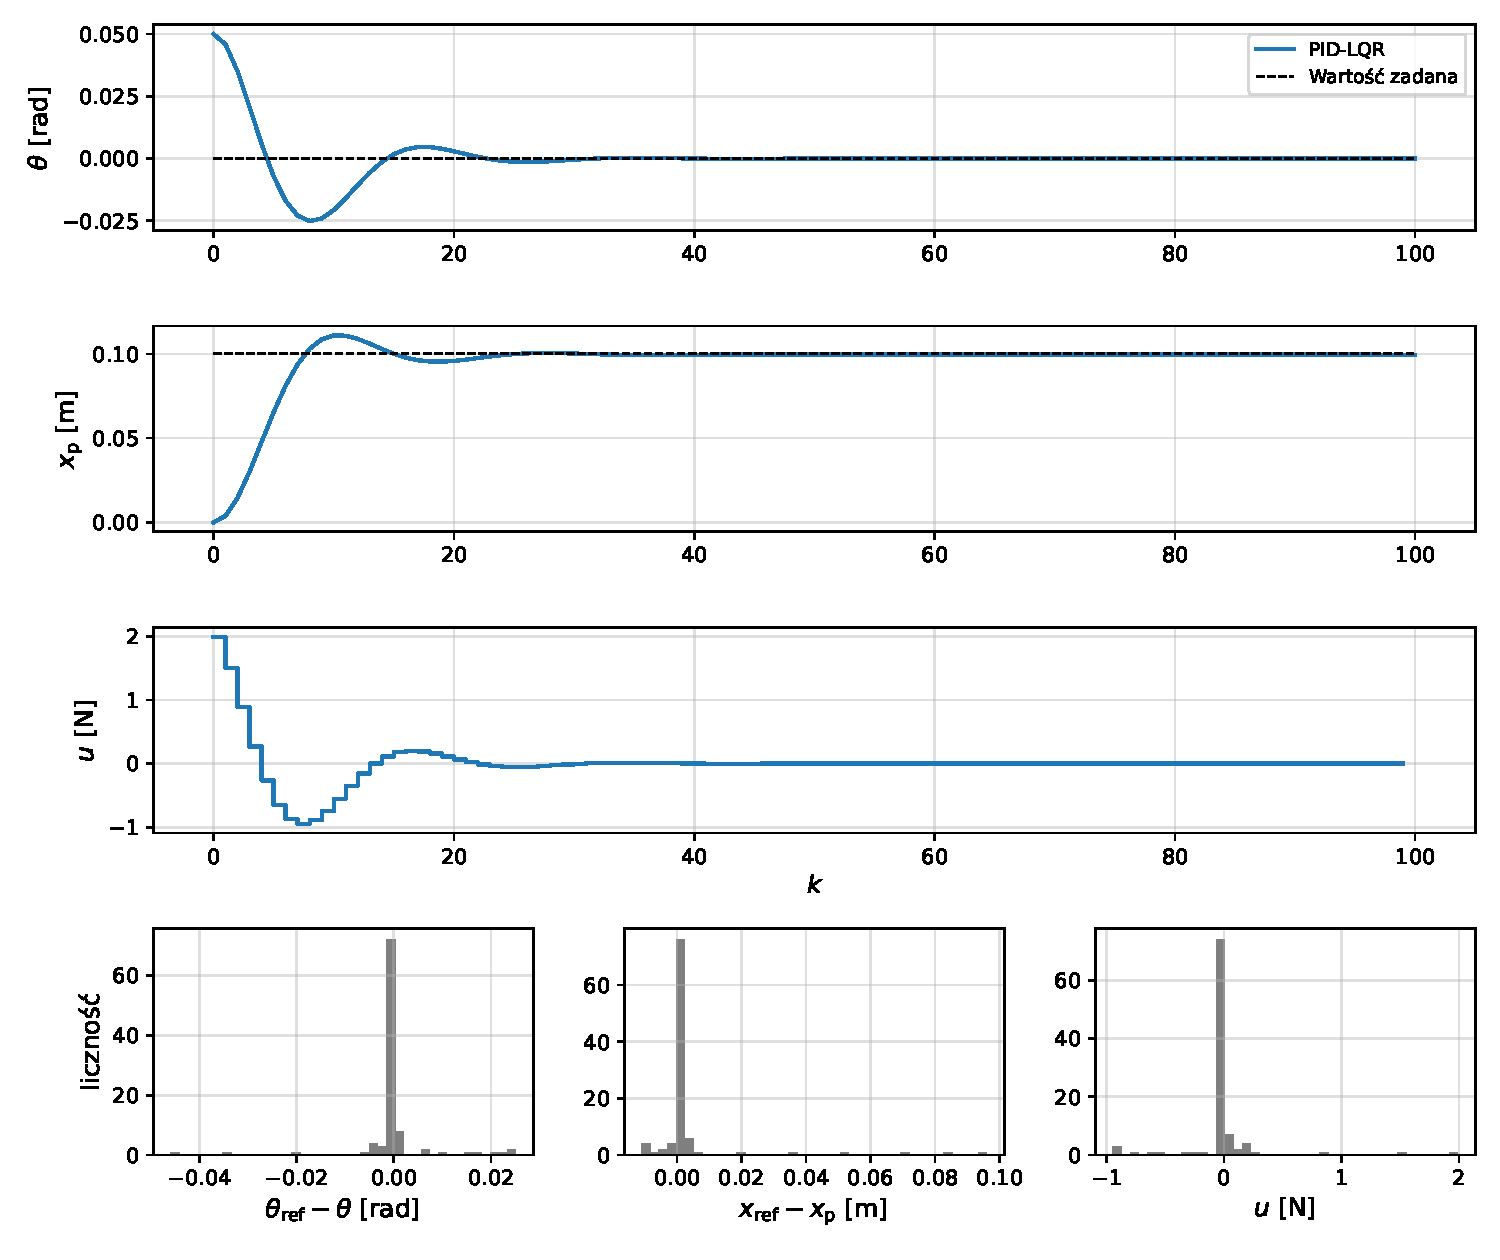
\includegraphics[width=\linewidth]{figs/S1_pid_lqr.pdf}
\caption{PID-LQR, Scenariusz S1 (nominalny): status automatyczny -- stabilny.}
\end{figure}
\clearpage
\begin{figure}[p]\centering
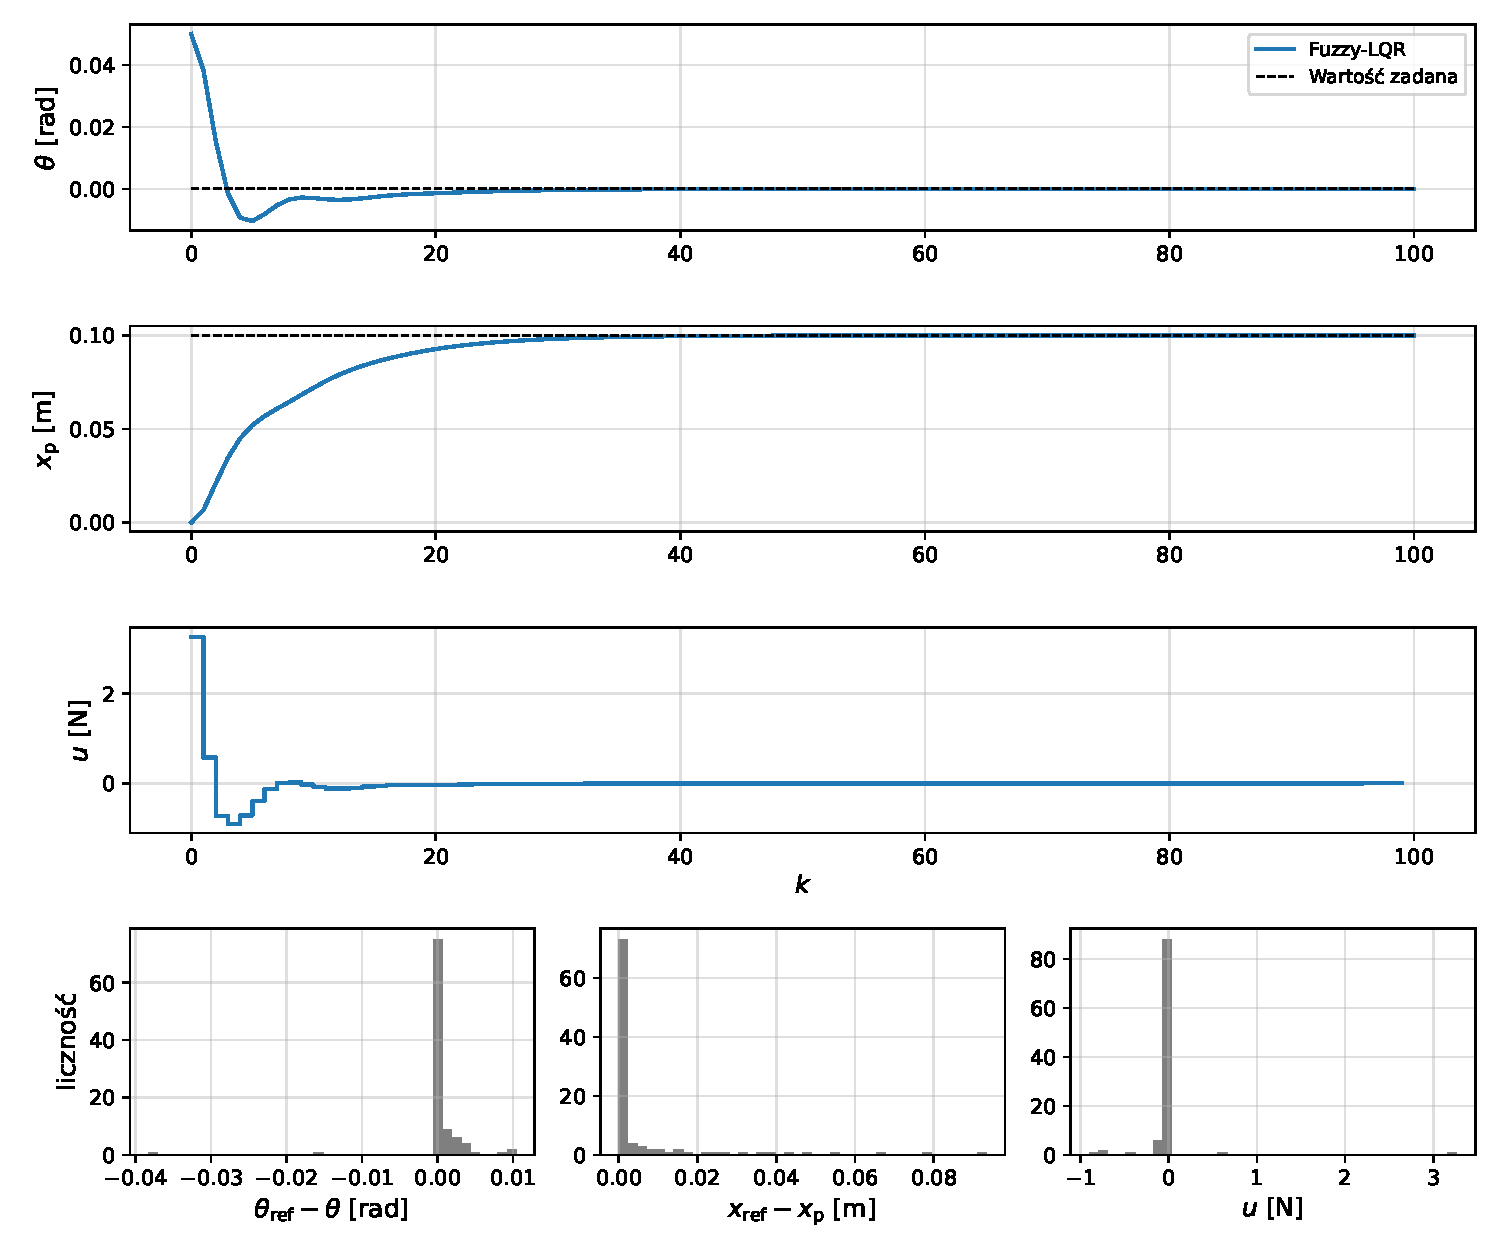
\includegraphics[width=\linewidth]{figs/S1_fuzzy_lqr.pdf}
\caption{Fuzzy-LQR, Scenariusz S1 (nominalny): status automatyczny -- stabilny.}
\end{figure}
\clearpage
\begin{figure}[p]\centering
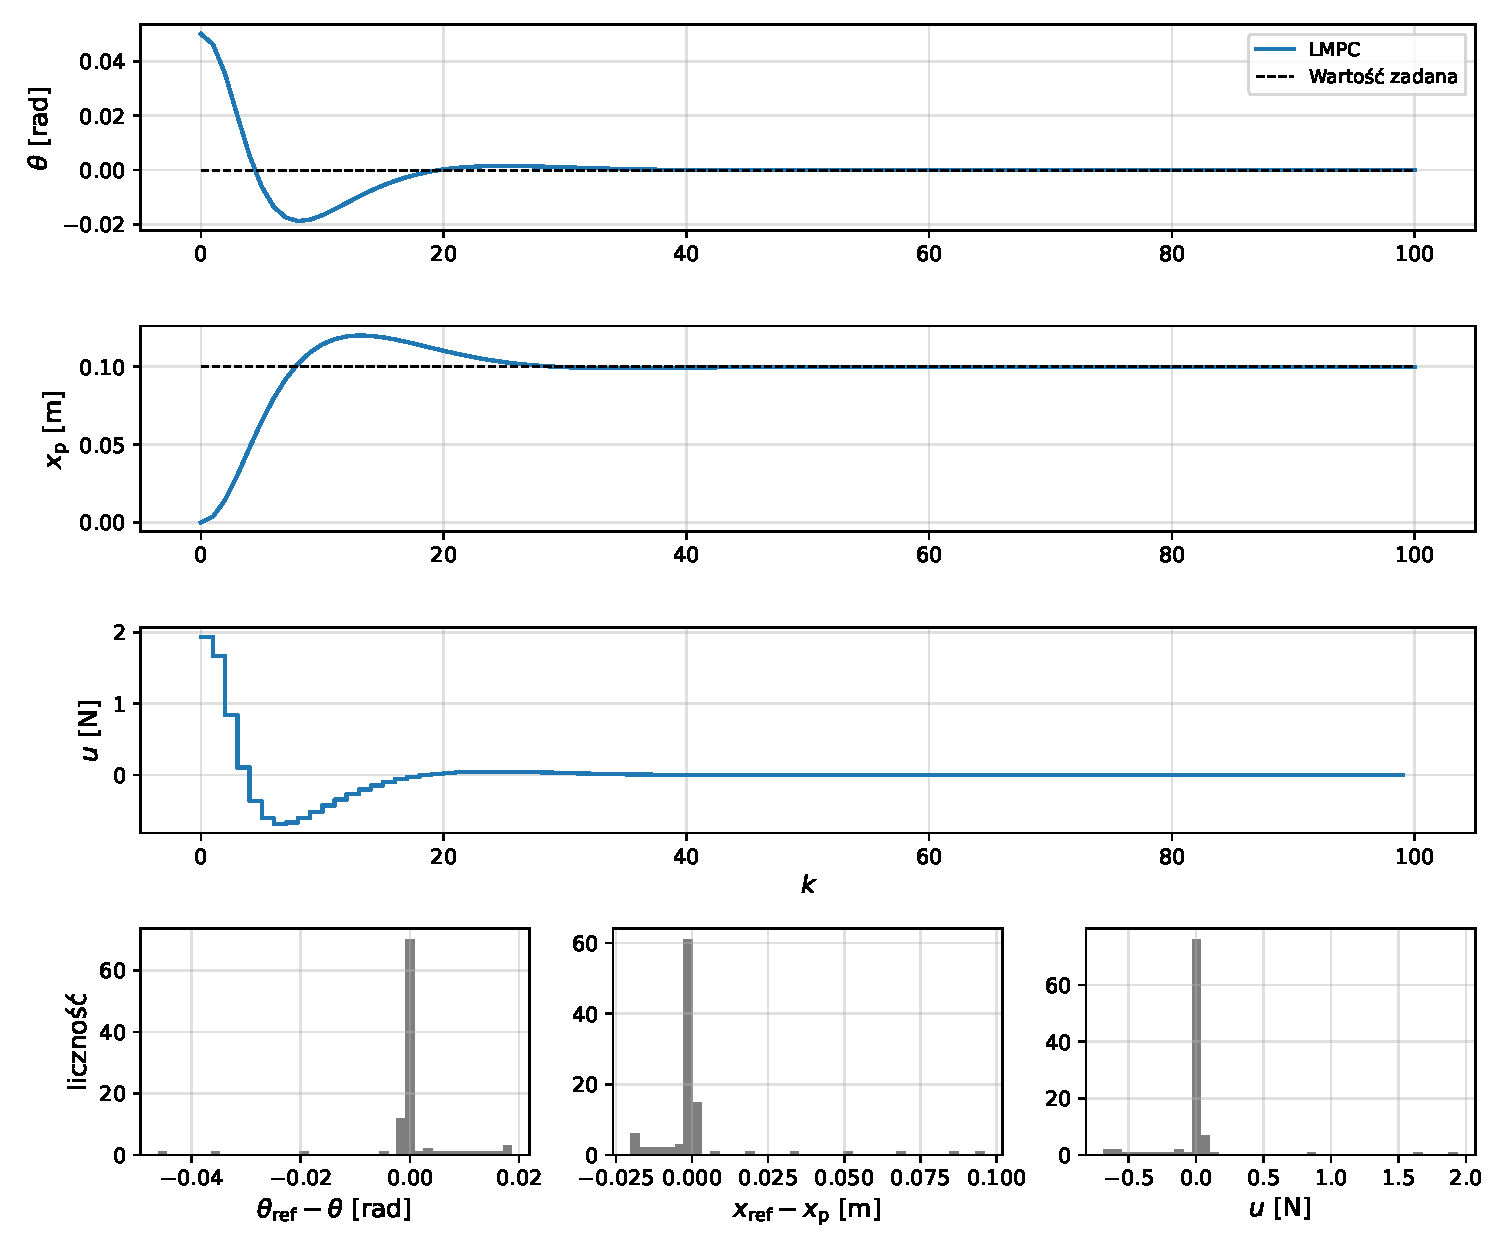
\includegraphics[width=\linewidth]{figs/S1_lmpc.pdf}
\caption{LMPC, Scenariusz S1 (nominalny): status automatyczny -- stabilny.}
\end{figure}
\clearpage
\begin{figure}[p]\centering
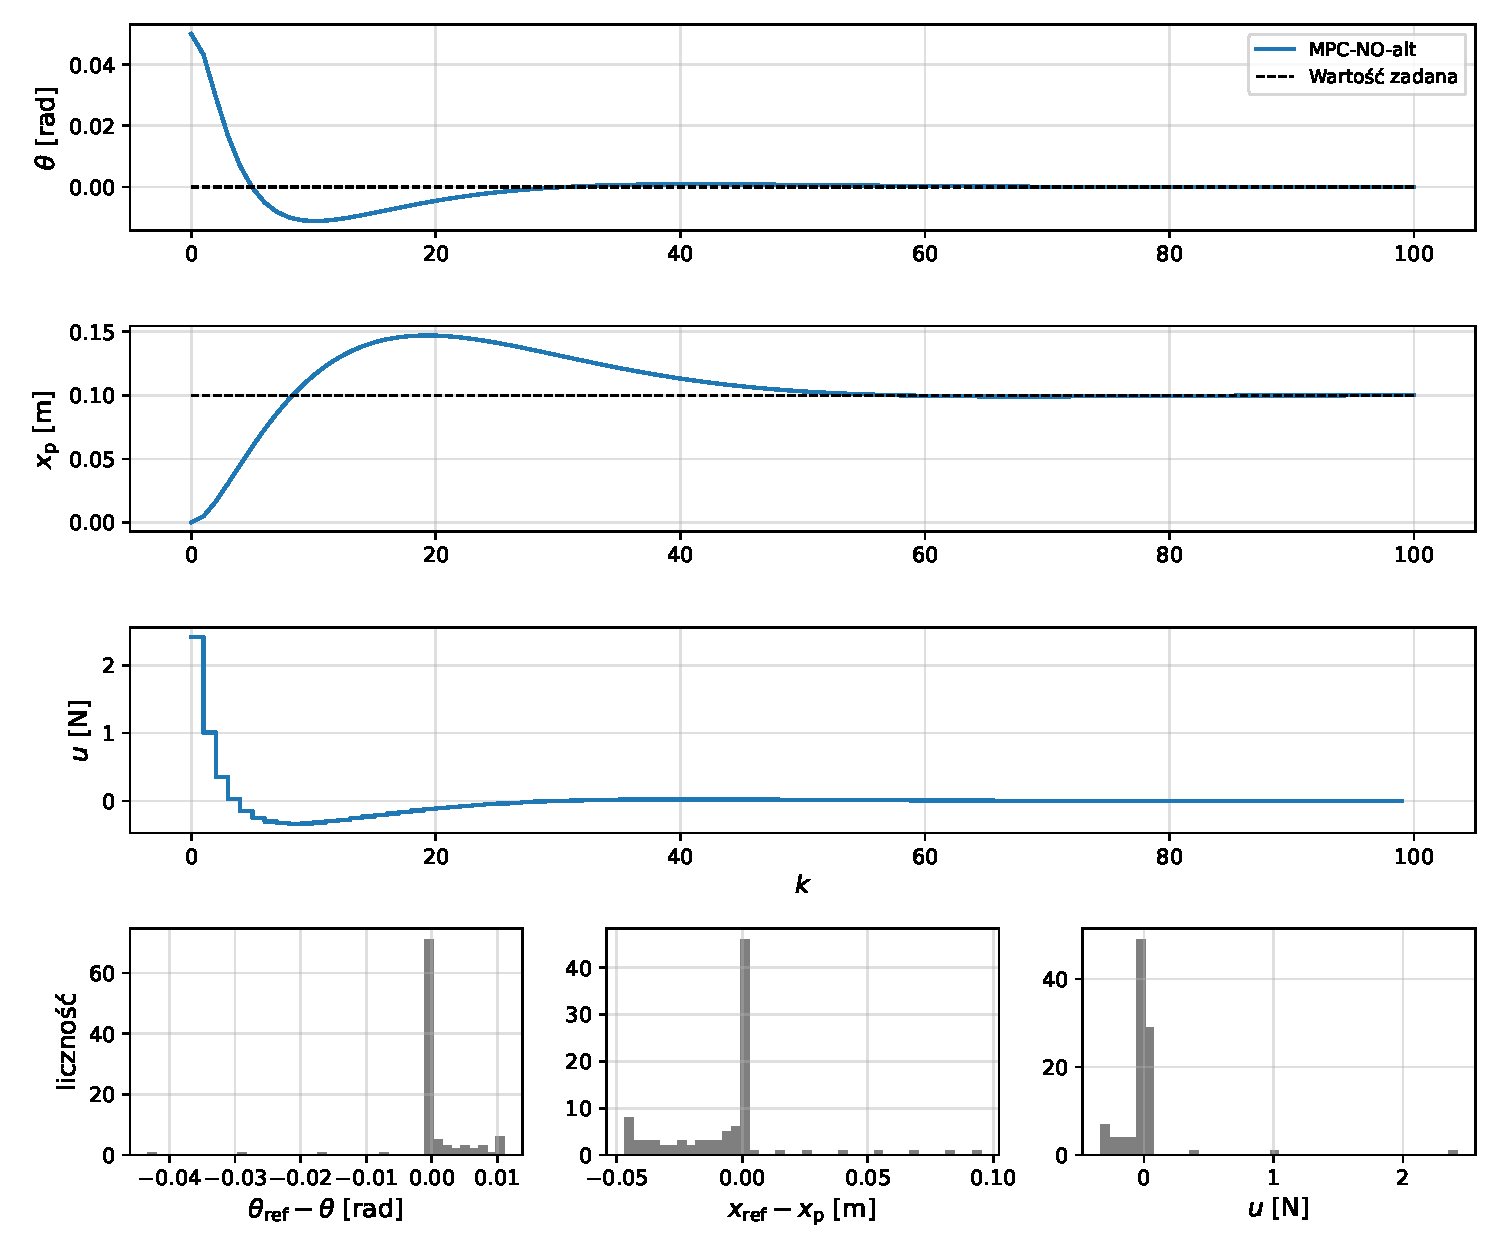
\includegraphics[width=\linewidth]{figs/S1_mpc_no_alt.pdf}
\caption{MPC-NO-alt, Scenariusz S1 (nominalny): status automatyczny -- stabilny.}
\end{figure}
\clearpage
\begin{figure}[p]\centering
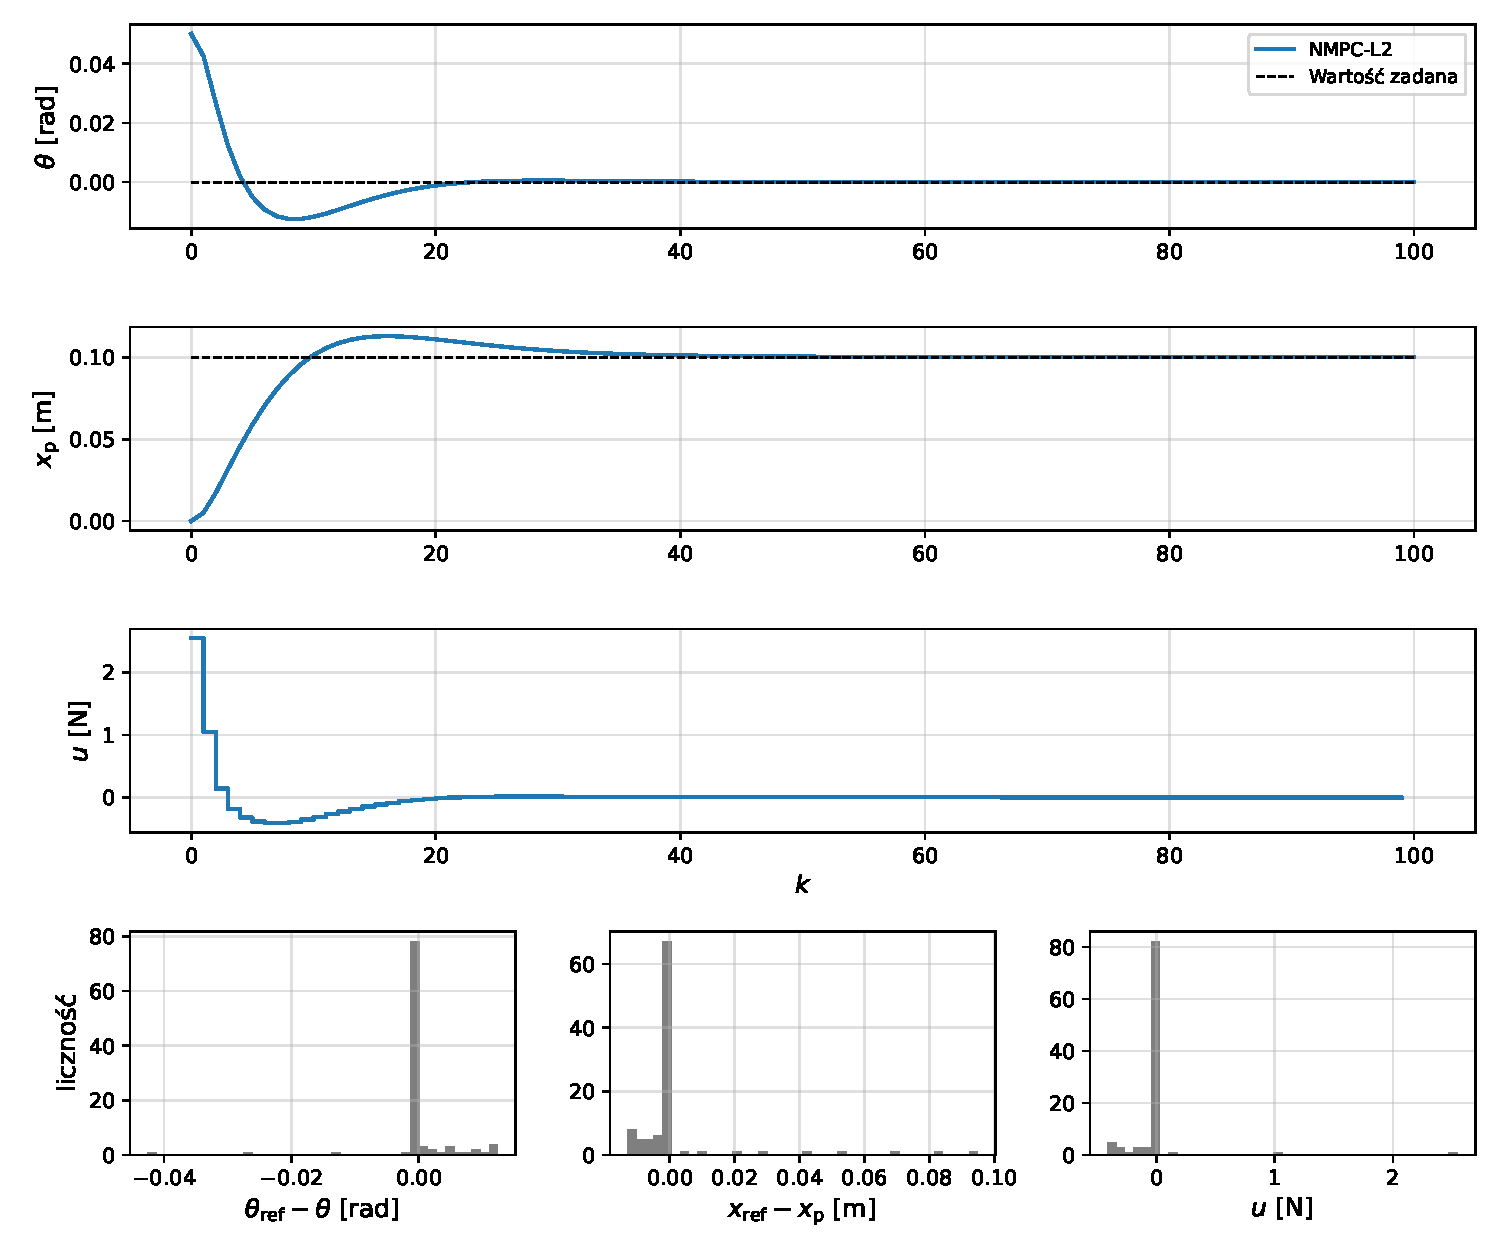
\includegraphics[width=\linewidth]{figs/S1_nmpc_l2.pdf}
\caption{NMPC-L$_2$, Scenariusz S1 (nominalny): status automatyczny -- stabilny.}
\end{figure}
\clearpage
\begin{figure}[p]\centering
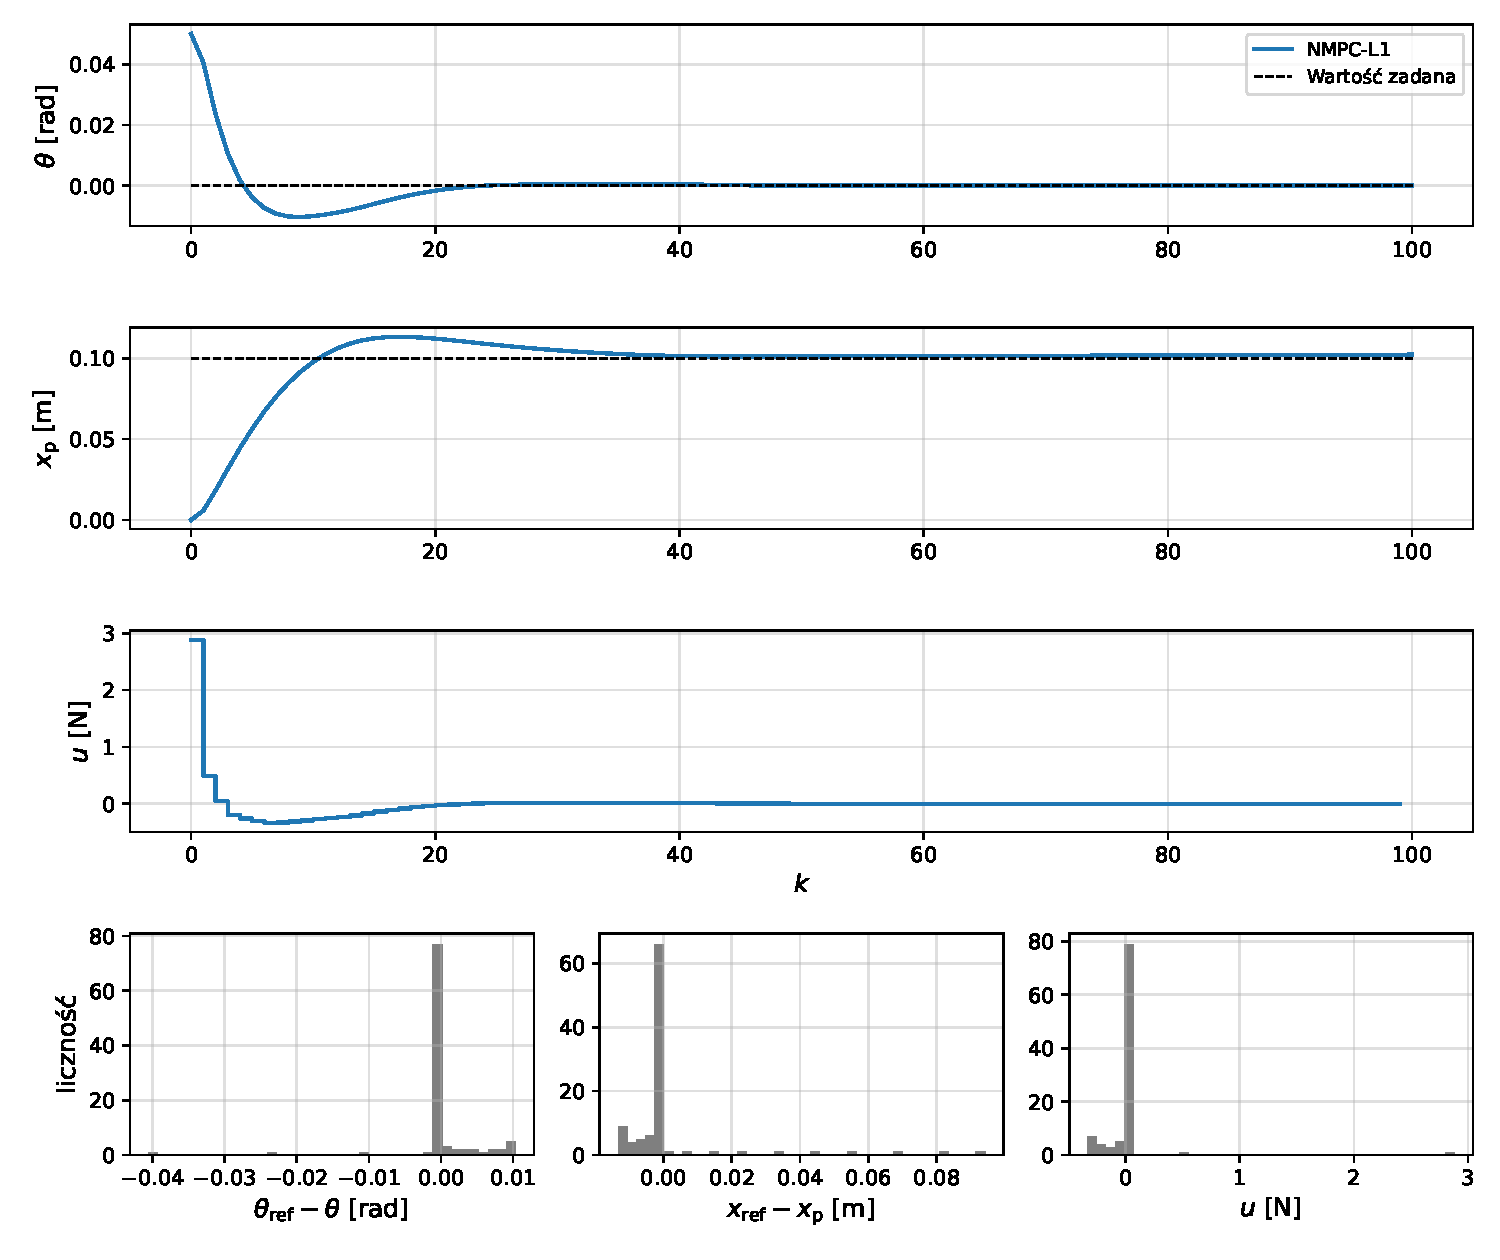
\includegraphics[width=\linewidth]{figs/S1_nmpc_l1.pdf}
\caption{NMPC-L$_1$, Scenariusz S1 (nominalny): status automatyczny -- stabilny.}
\end{figure}
\clearpage
\begin{figure}[p]\centering
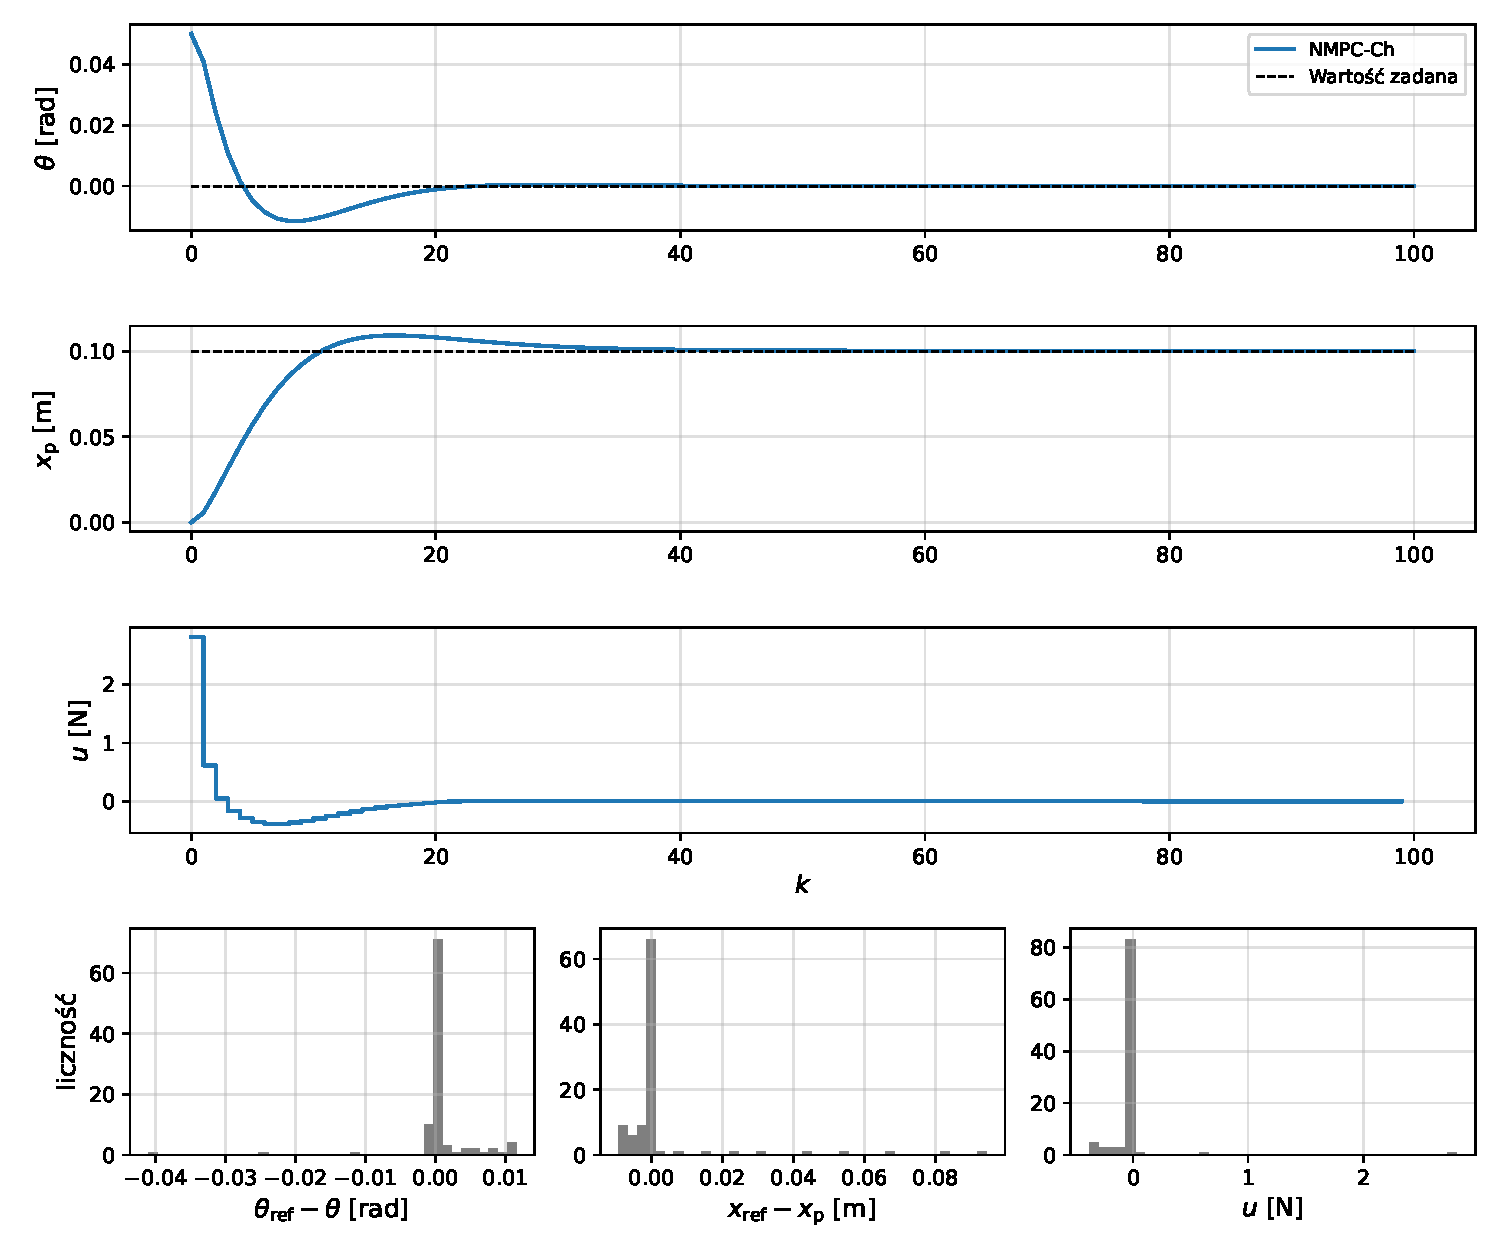
\includegraphics[width=\linewidth]{figs/S1_nmpc_ch.pdf}
\caption{NMPC-Ch, Scenariusz S1 (nominalny): status automatyczny -- stabilny.}
\end{figure}
\clearpage
\begin{figure}[p]\centering
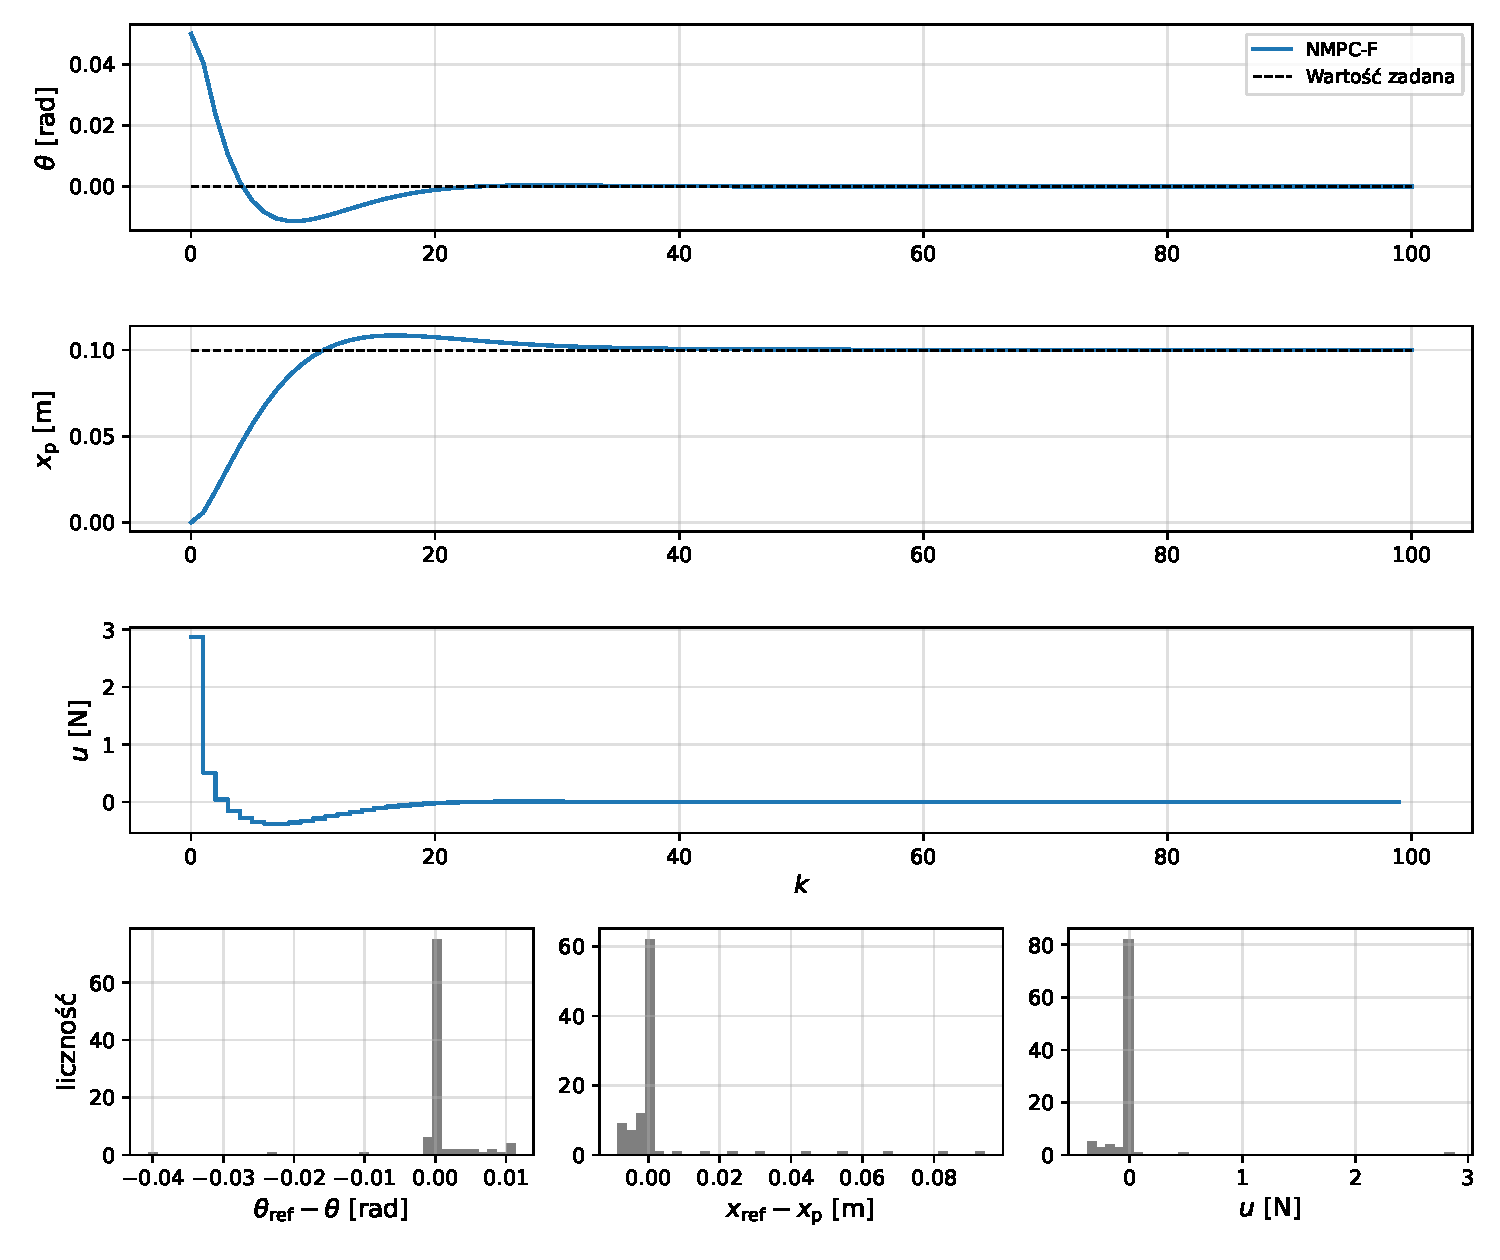
\includegraphics[width=\linewidth]{figs/S1_nmpc_f.pdf}
\caption{NMPC-F, Scenariusz S1 (nominalny): status automatyczny -- stabilny.}
\end{figure}
\clearpage
\begin{figure}[p]\centering
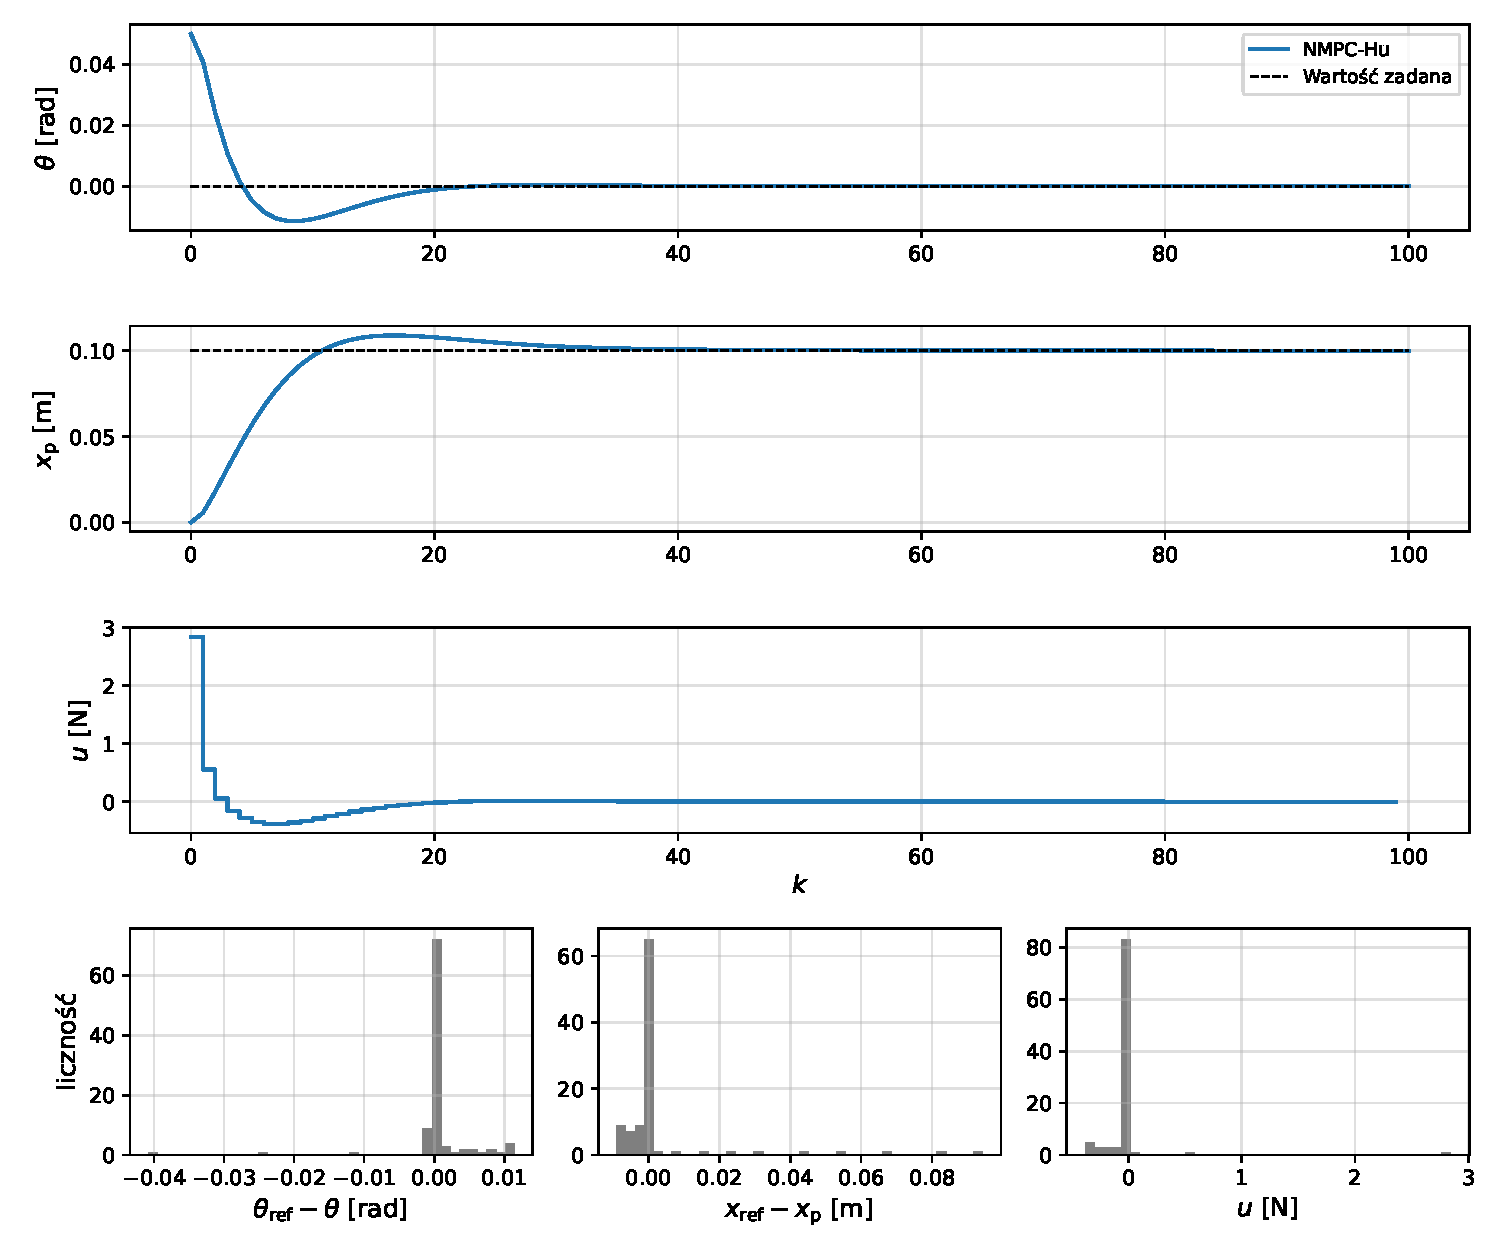
\includegraphics[width=\linewidth]{figs/S1_nmpc_hu.pdf}
\caption{NMPC-Hu, Scenariusz S1 (nominalny): status automatyczny -- stabilny.}
\end{figure}
\clearpage
\begin{figure}[p]\centering
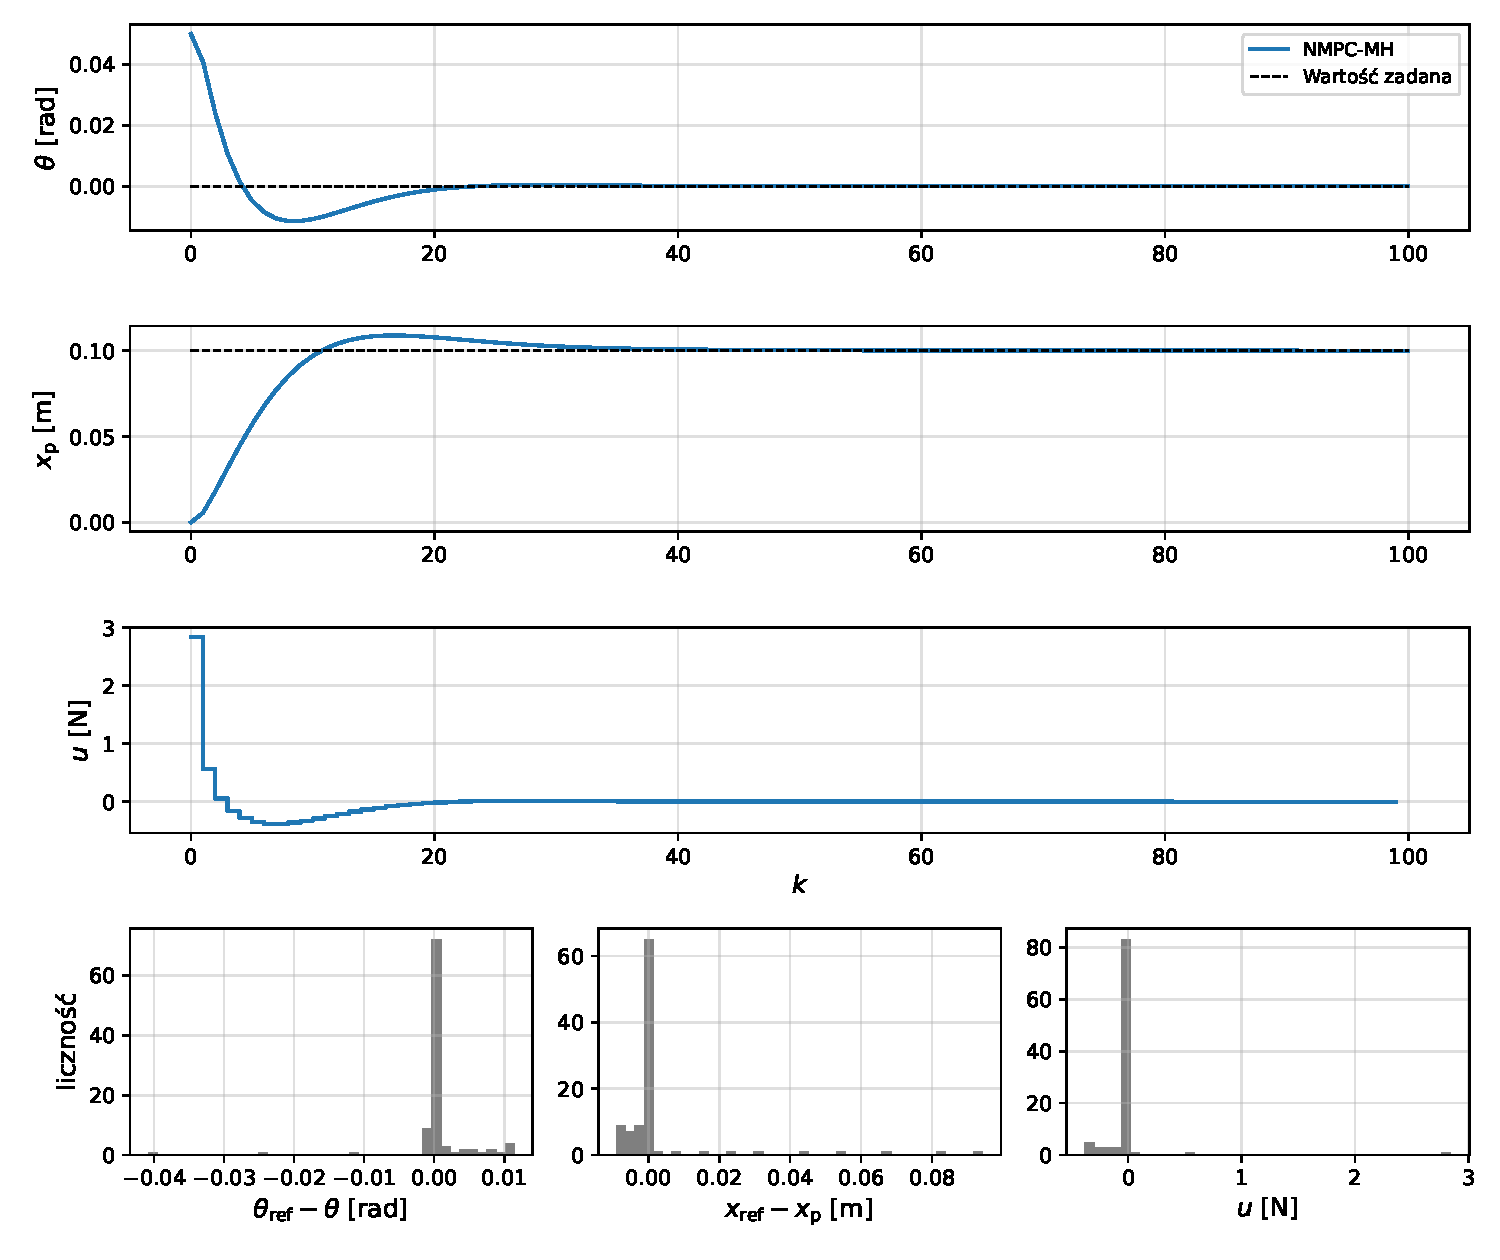
\includegraphics[width=\linewidth]{figs/S1_nmpc_mh.pdf}
\caption{NMPC-MH, Scenariusz S1 (nominalny): status automatyczny -- stabilny.}
\end{figure}
\clearpage
\begin{figure}[p]\centering
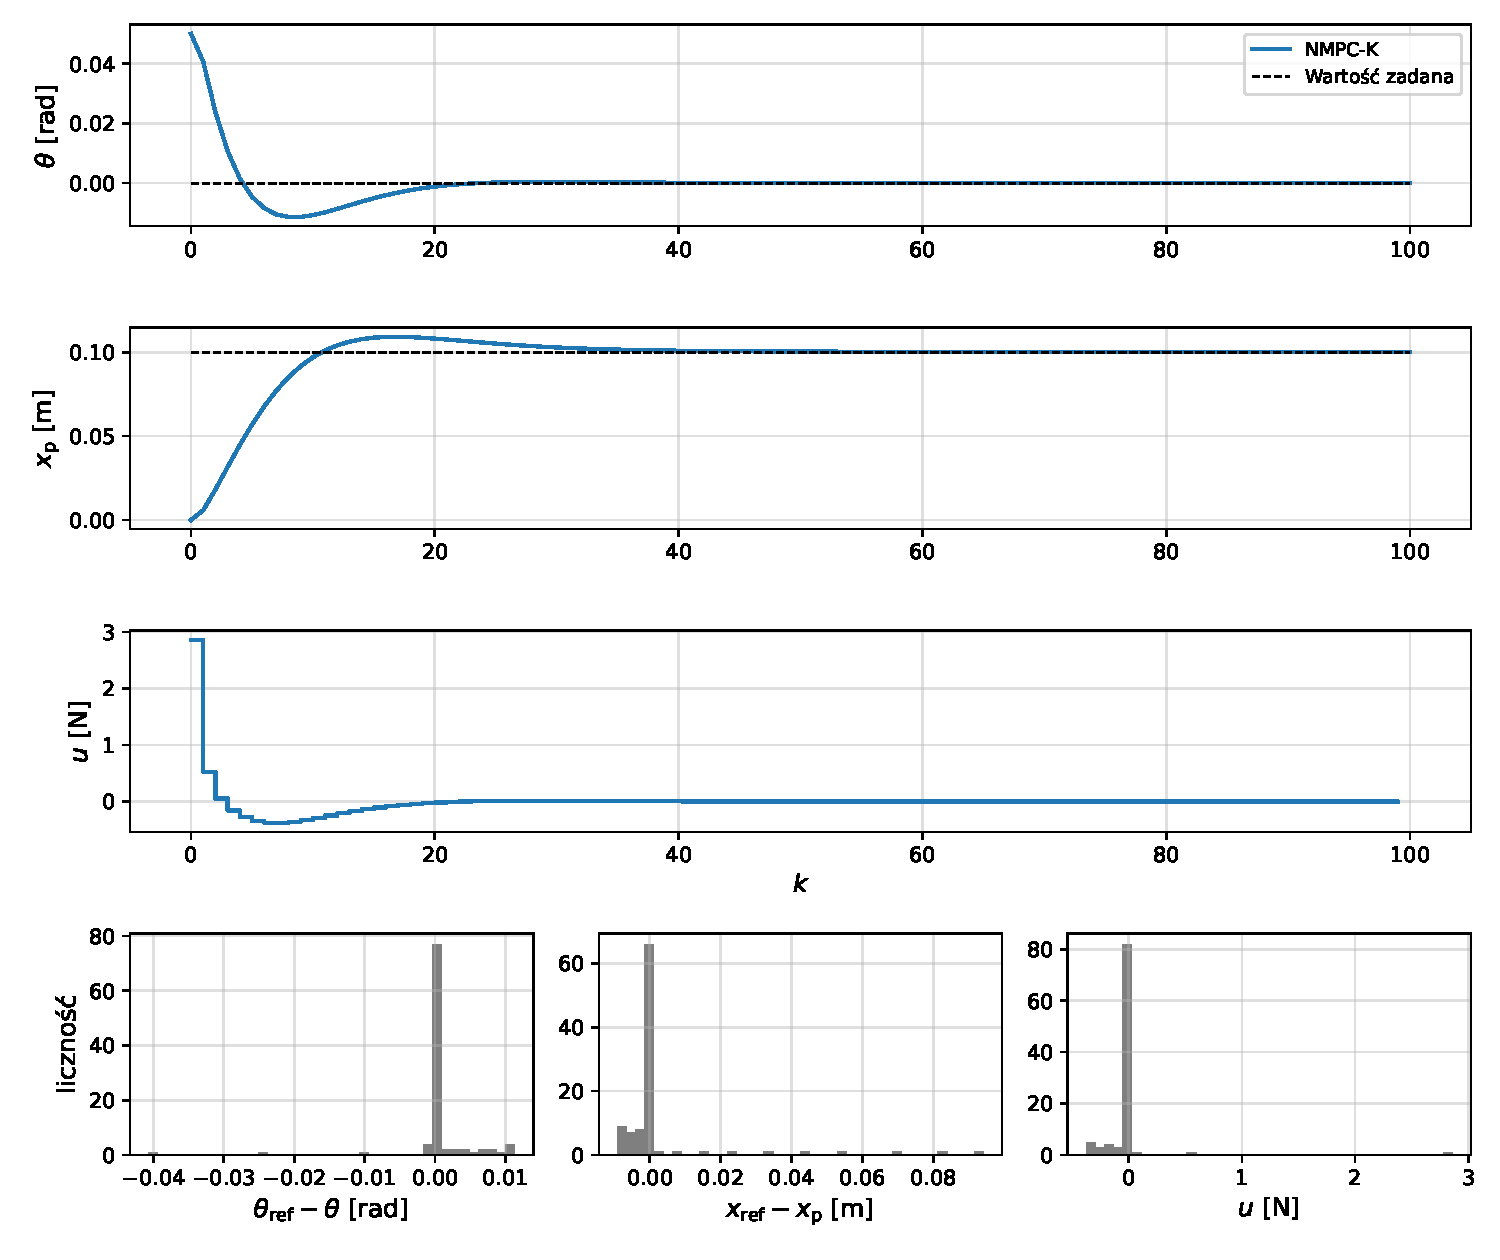
\includegraphics[width=\linewidth]{figs/S1_nmpc_k.pdf}
\caption{NMPC-K, Scenariusz S1 (nominalny): status automatyczny -- stabilny.}
\end{figure}
\clearpage
\begin{figure}[p]\centering
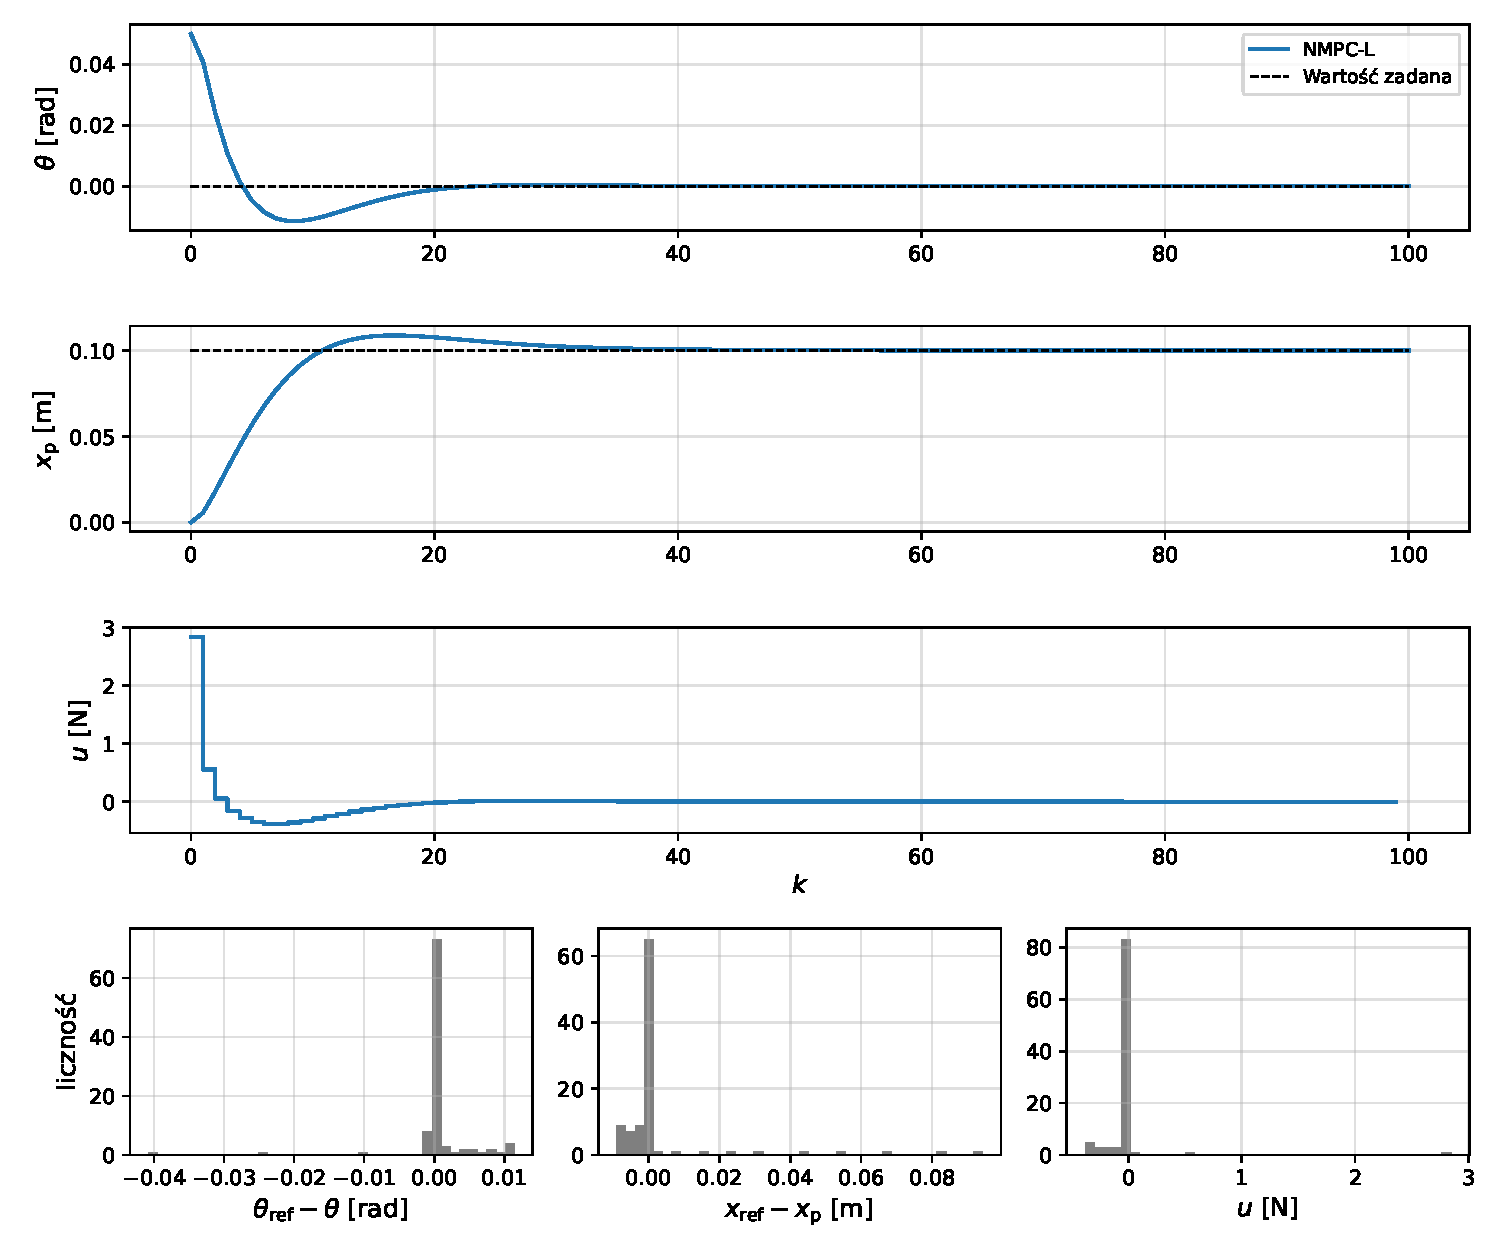
\includegraphics[width=\linewidth]{figs/S1_nmpc_l.pdf}
\caption{NMPC-L, Scenariusz S1 (nominalny): status automatyczny -- stabilny.}
\end{figure}
\clearpage
\begin{figure}[p]\centering
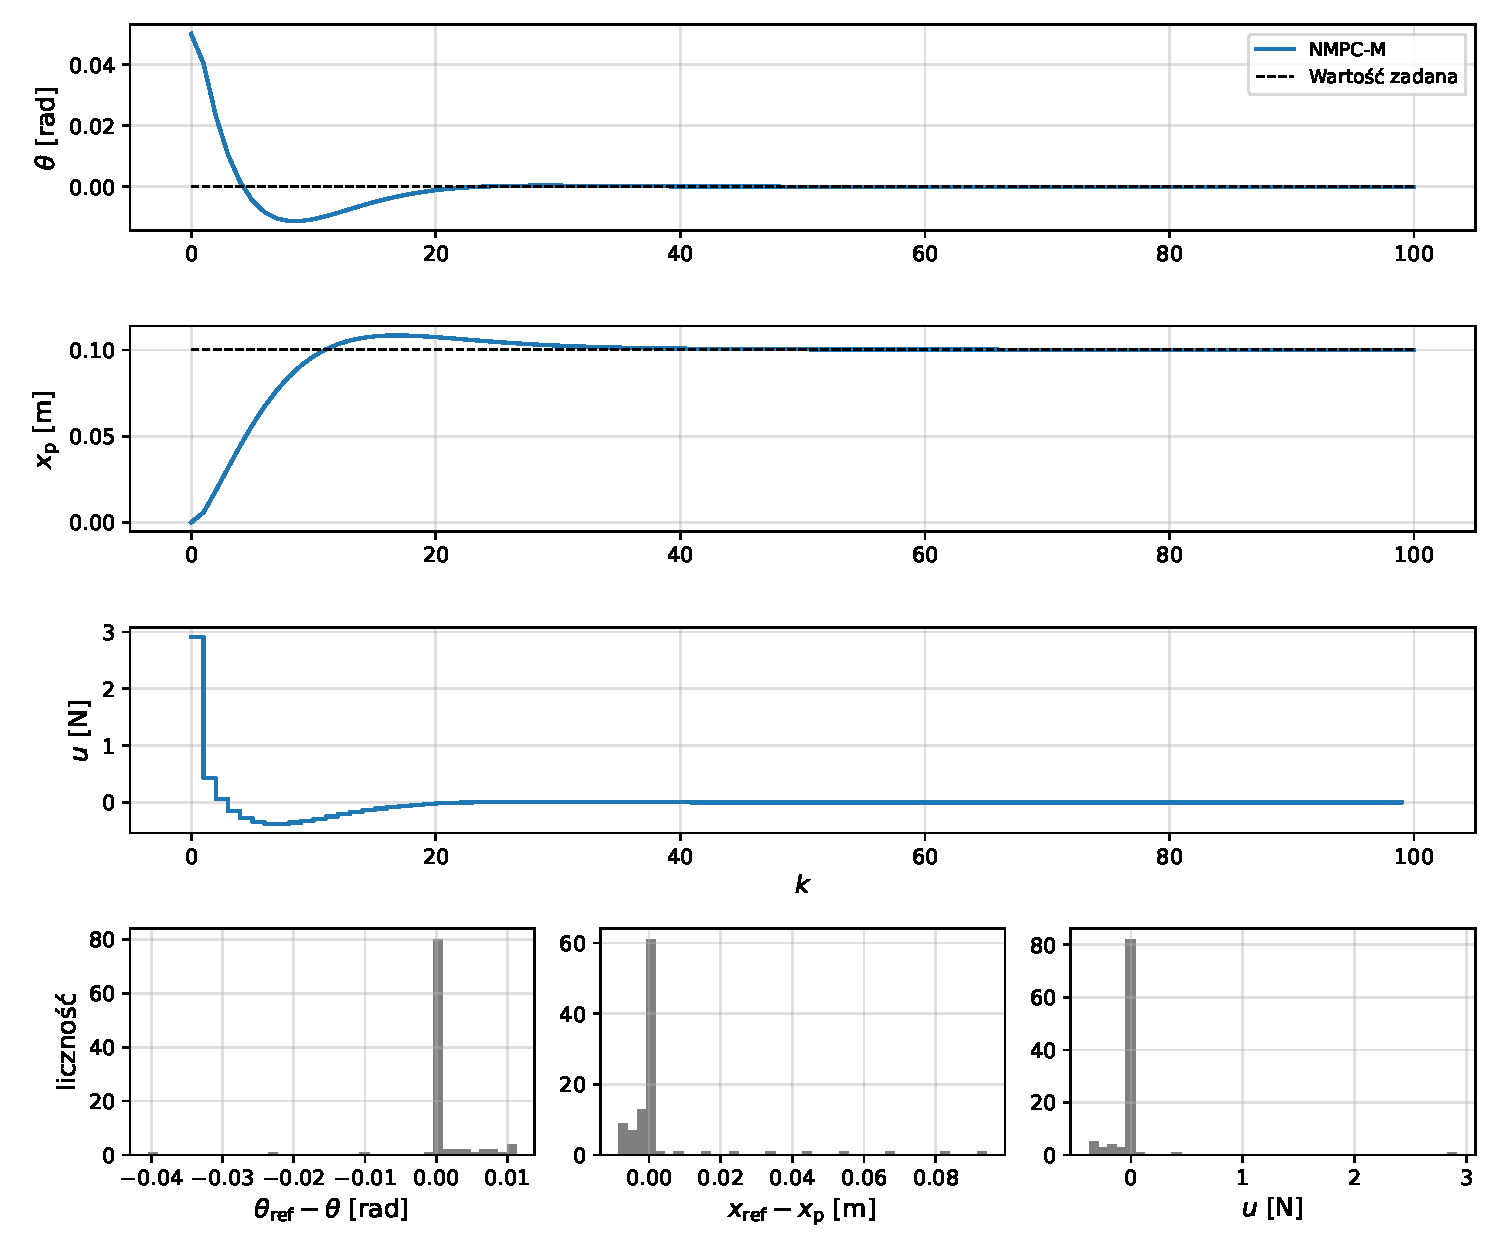
\includegraphics[width=\linewidth]{figs/S1_nmpc_m.pdf}
\caption{NMPC-M, Scenariusz S1 (nominalny): status automatyczny -- stabilny.}
\end{figure}
\clearpage
\begin{figure}[p]\centering
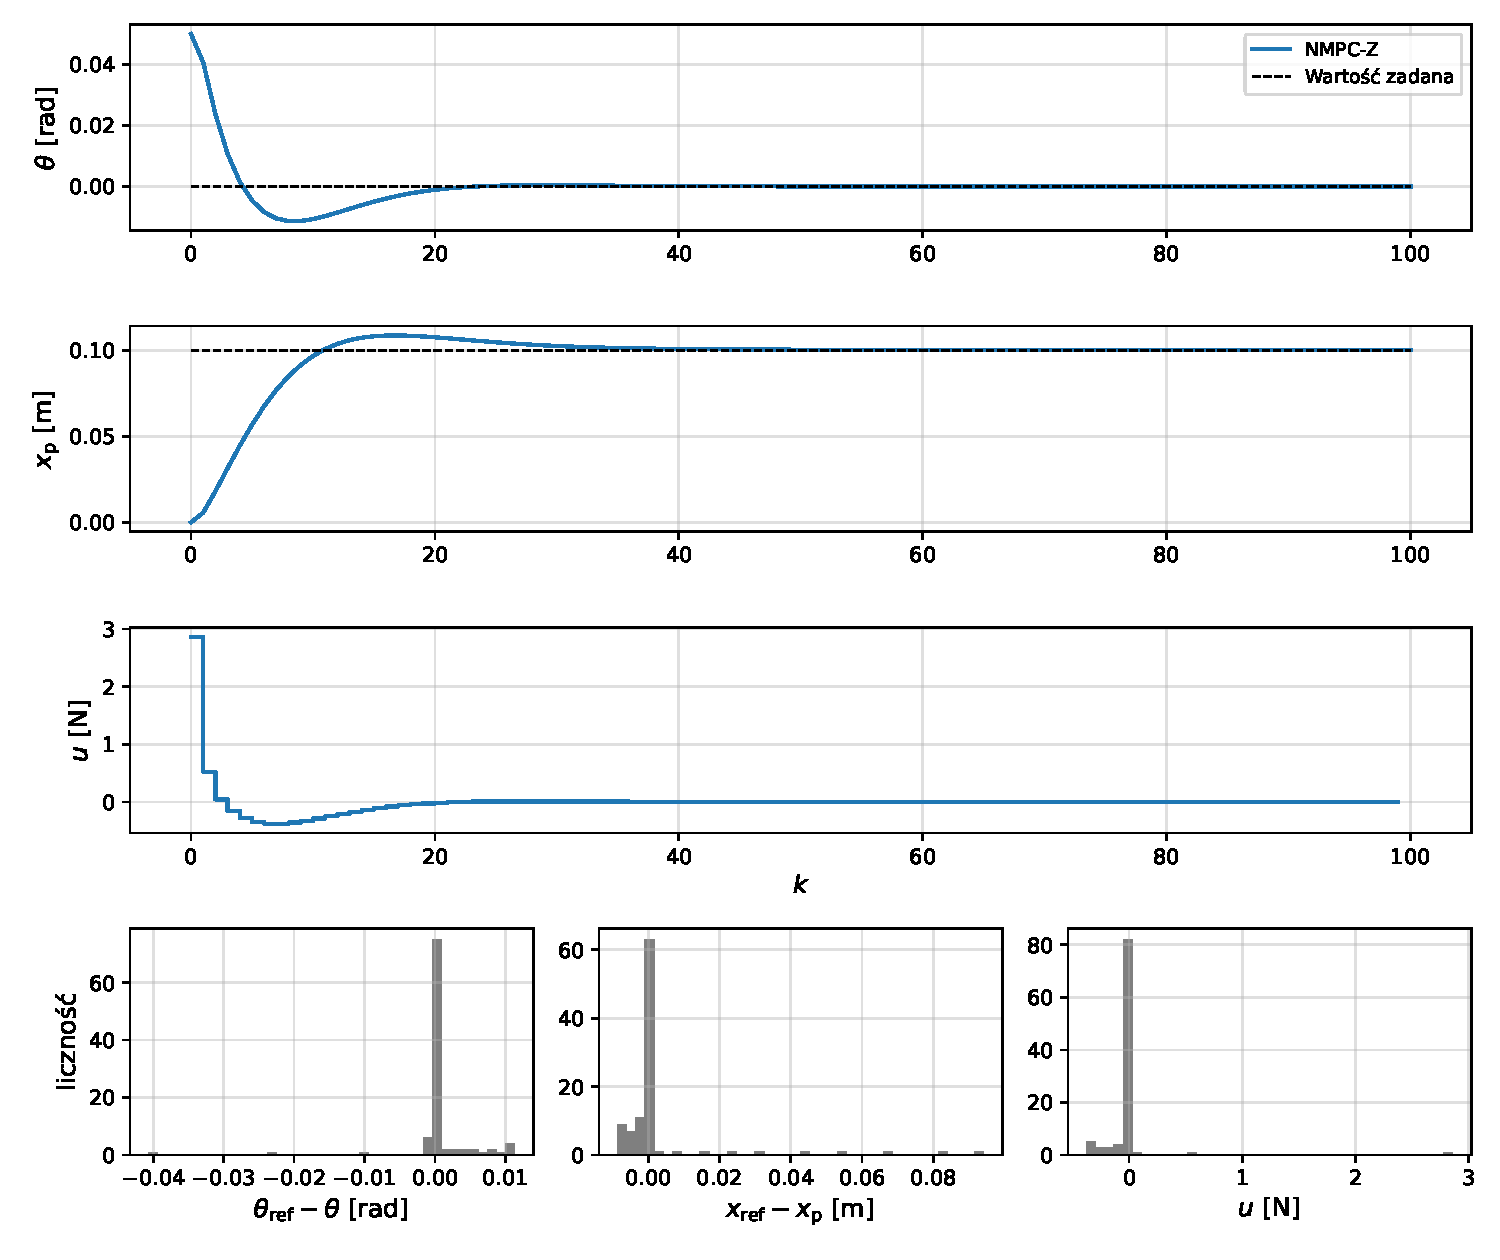
\includegraphics[width=\linewidth]{figs/S1_nmpc_z.pdf}
\caption{NMPC-Z, Scenariusz S1 (nominalny): status automatyczny -- stabilny.}
\end{figure}
\clearpage
\begin{figure}[p]\centering
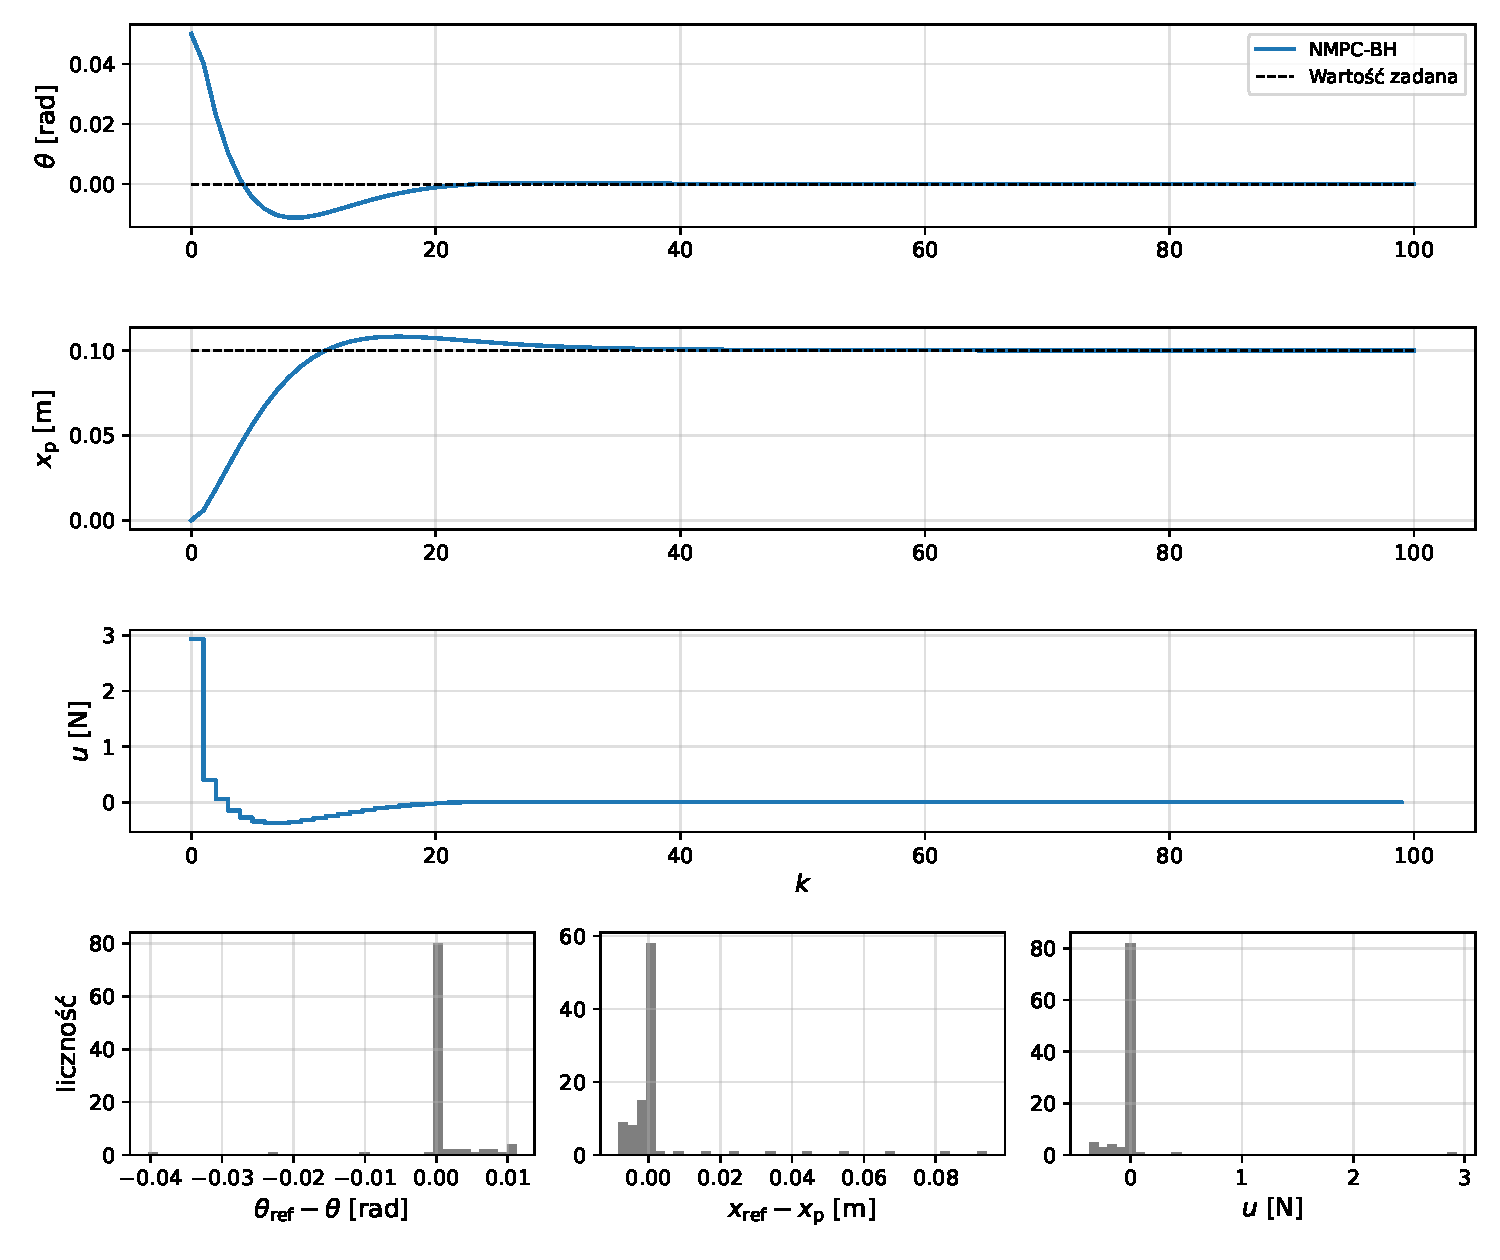
\includegraphics[width=\linewidth]{figs/S1_nmpc_bh.pdf}
\caption{NMPC-BH, Scenariusz S1 (nominalny): status automatyczny -- stabilny.}
\end{figure}
\clearpage
\begin{figure}[p]\centering
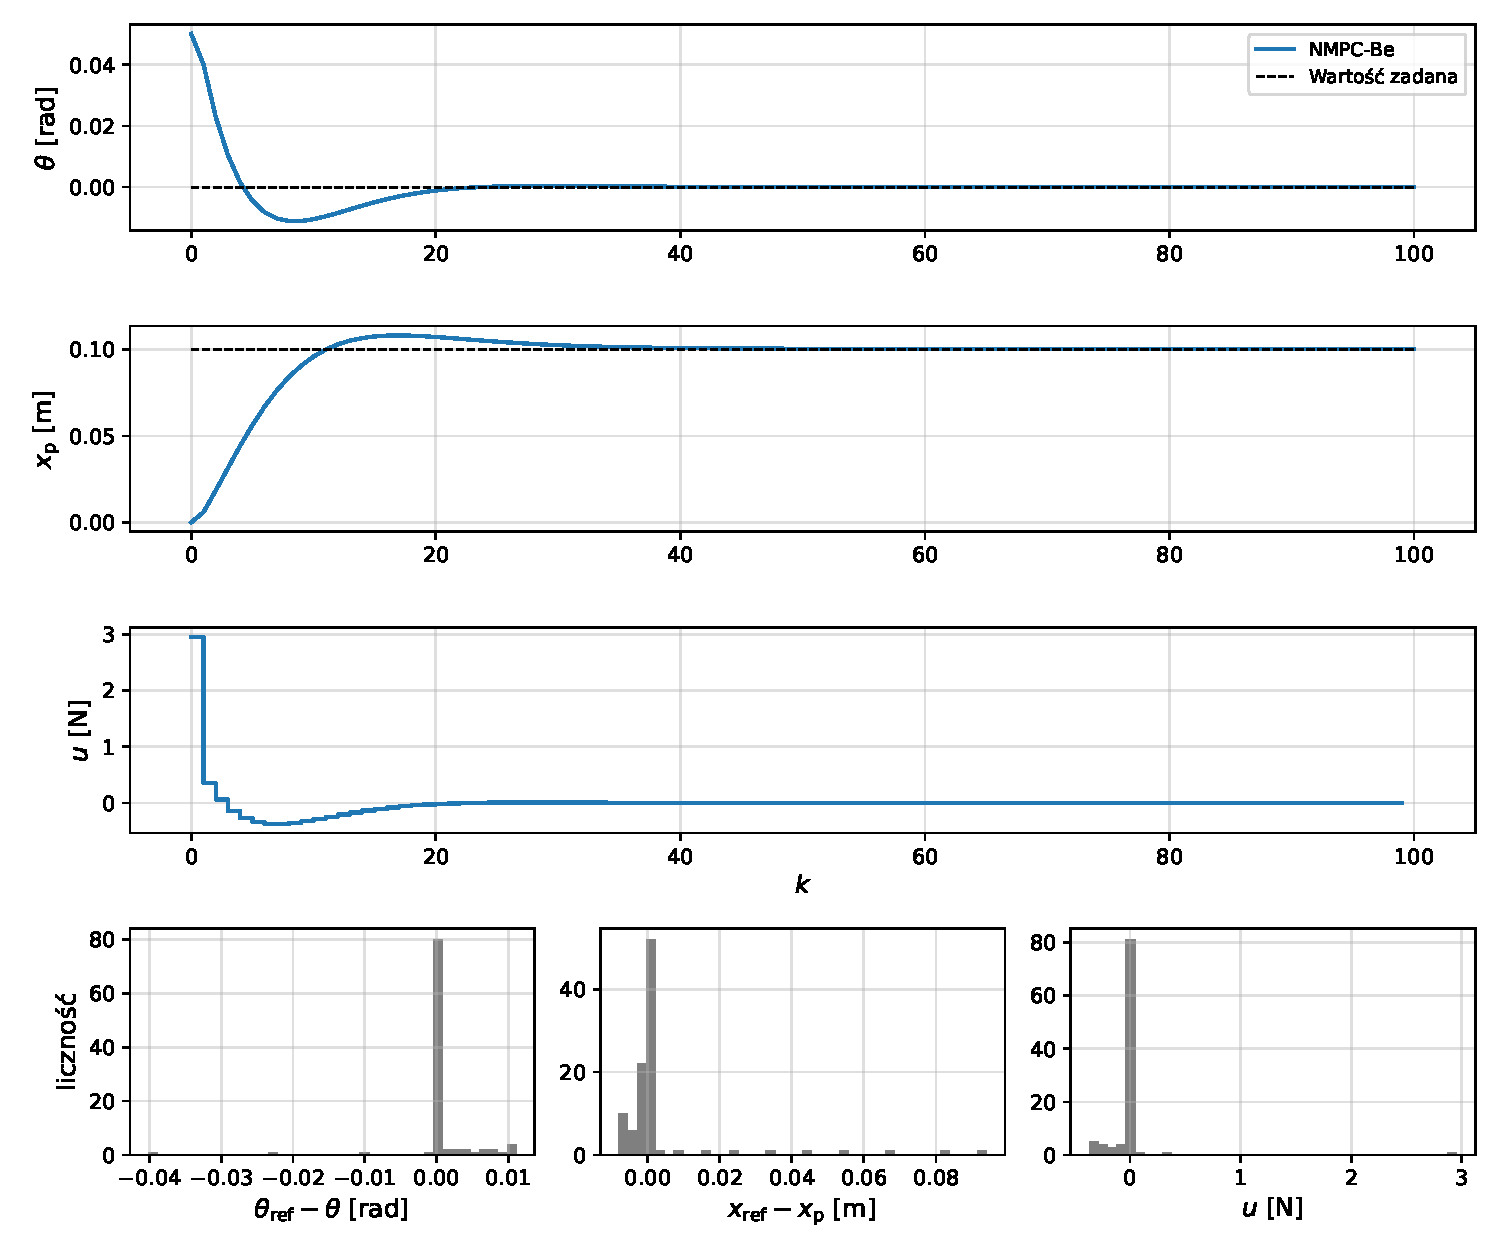
\includegraphics[width=\linewidth]{figs/S1_nmpc_be.pdf}
\caption{NMPC-Be, Scenariusz S1 (nominalny): status automatyczny -- stabilny.}
\end{figure}
\clearpage
\begin{figure}[p]\centering
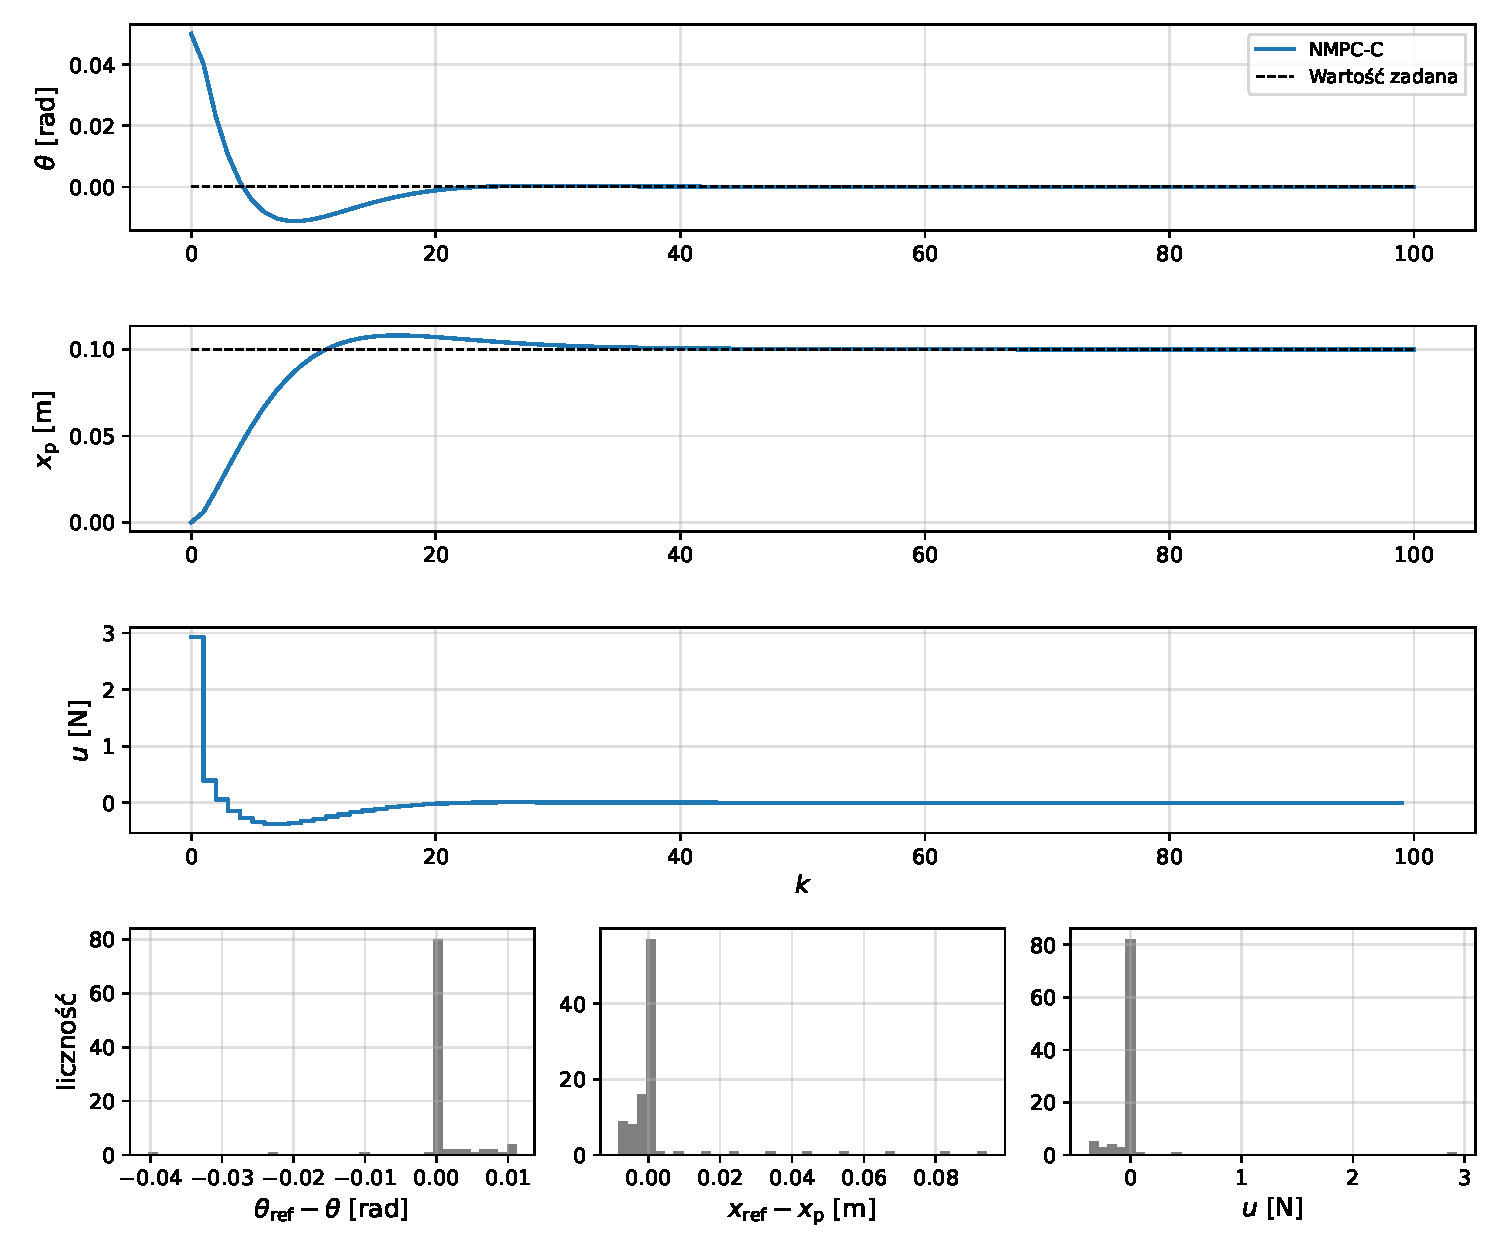
\includegraphics[width=\linewidth]{figs/S1_nmpc_c.pdf}
\caption{NMPC-C, Scenariusz S1 (nominalny): status automatyczny -- stabilny.}
\end{figure}
\clearpage
\begin{figure}[p]\centering
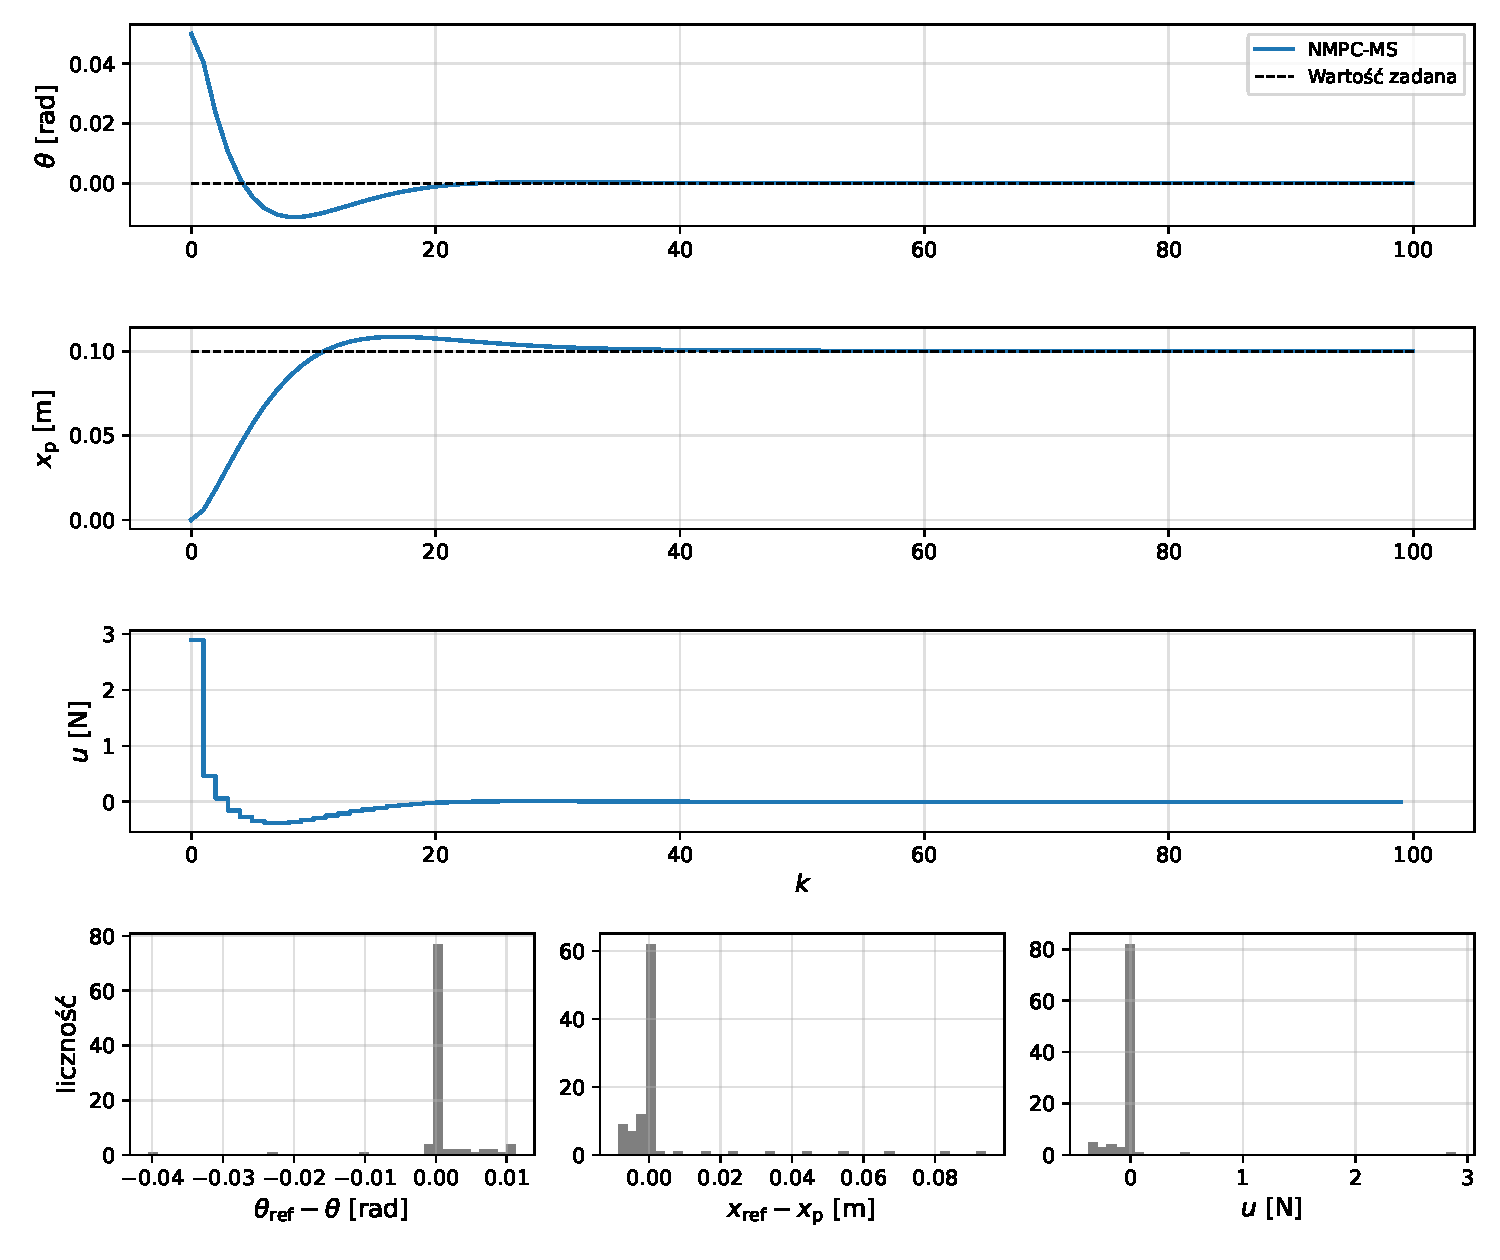
\includegraphics[width=\linewidth]{figs/S1_nmpc_ms.pdf}
\caption{NMPC-MS, Scenariusz S1 (nominalny): status automatyczny -- stabilny.}
\end{figure}
\clearpage
\begin{figure}[p]\centering
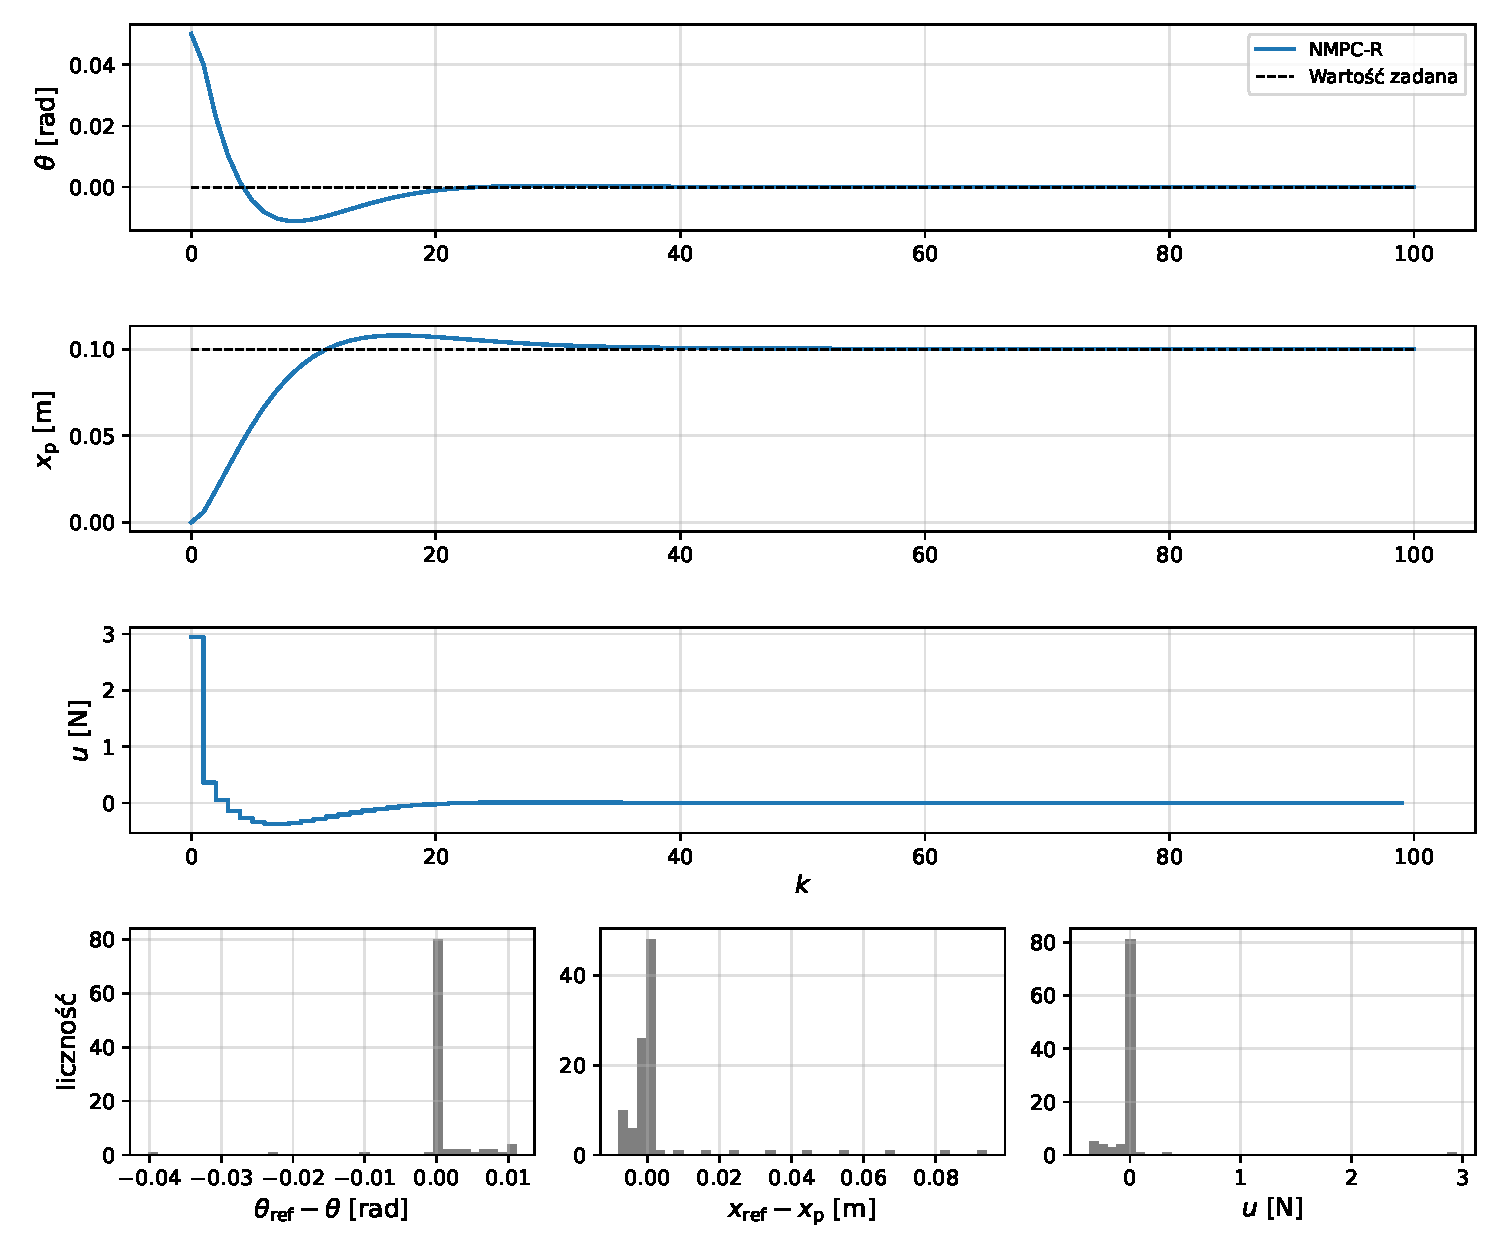
\includegraphics[width=\linewidth]{figs/S1_nmpc_r.pdf}
\caption{NMPC-R, Scenariusz S1 (nominalny): status automatyczny -- stabilny.}
\end{figure}
\clearpage
\begin{figure}[p]\centering
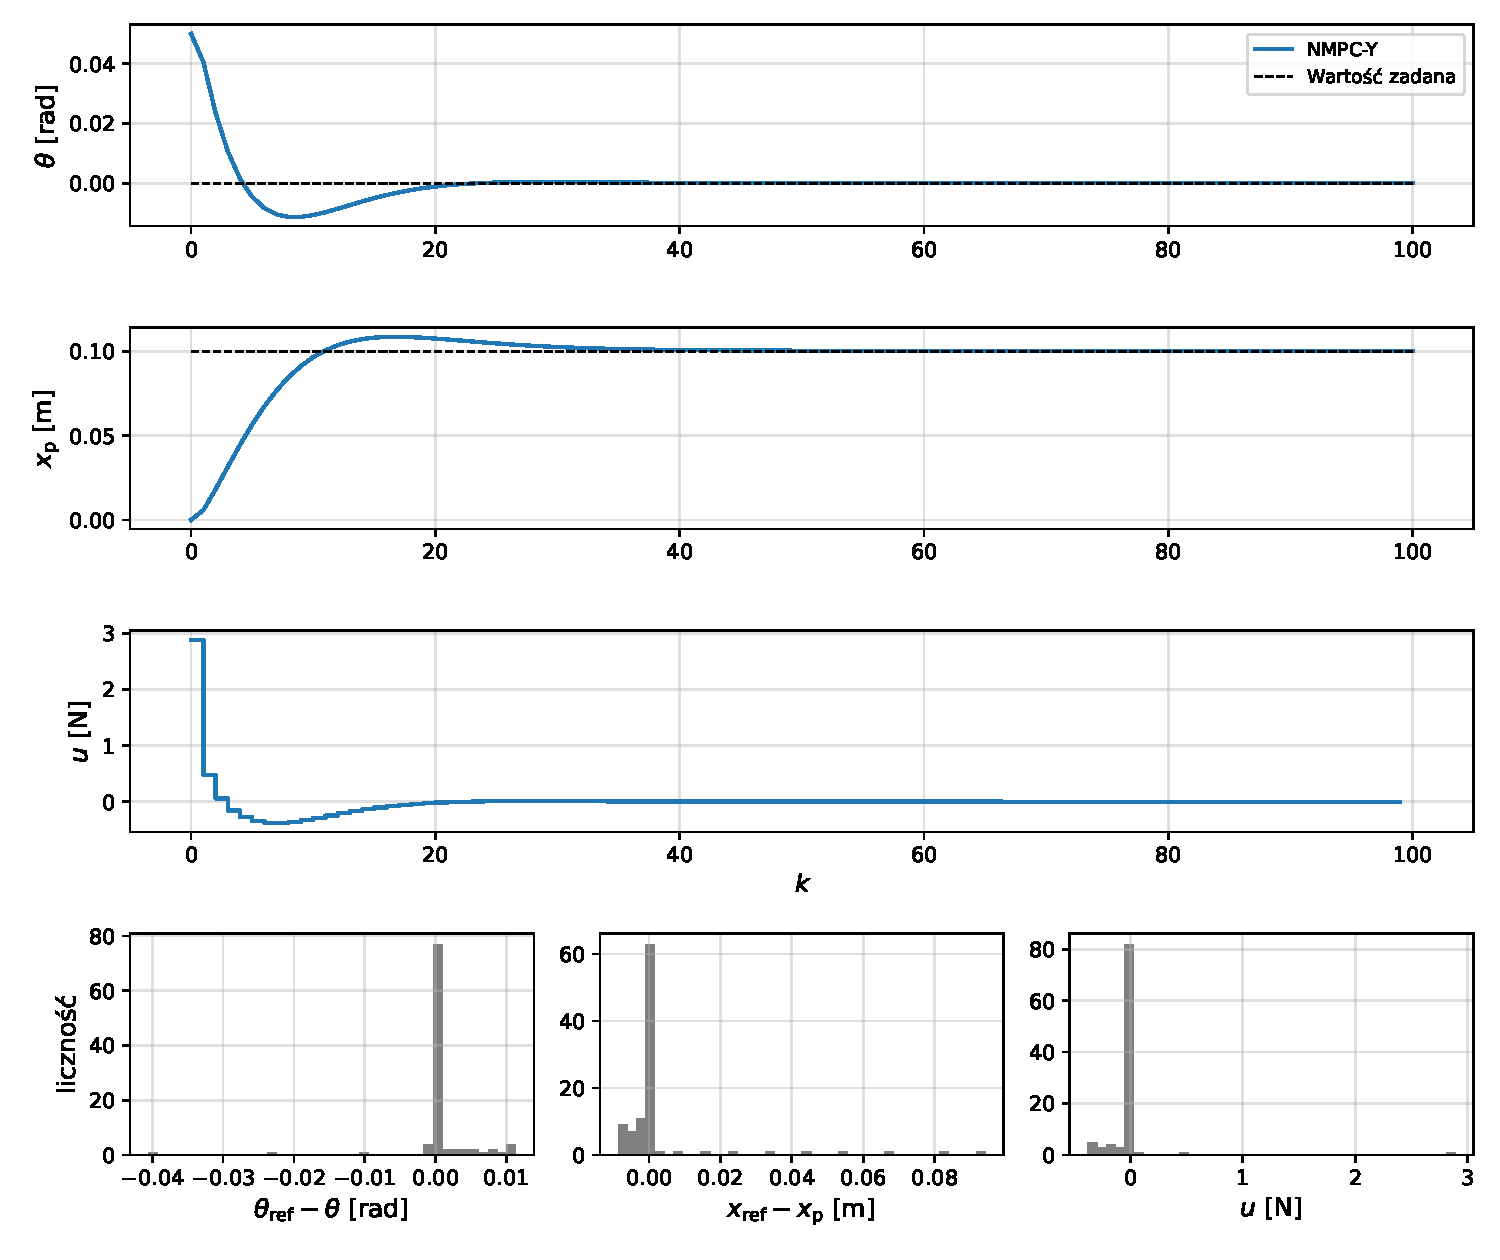
\includegraphics[width=\linewidth]{figs/S1_nmpc_y.pdf}
\caption{NMPC-Y, Scenariusz S1 (nominalny): status automatyczny -- stabilny.}
\end{figure}
\clearpage
\subsection{Przebiegi -- Scenariusz S2 (skoki zakłócenia)}
\begin{figure}[p]\centering
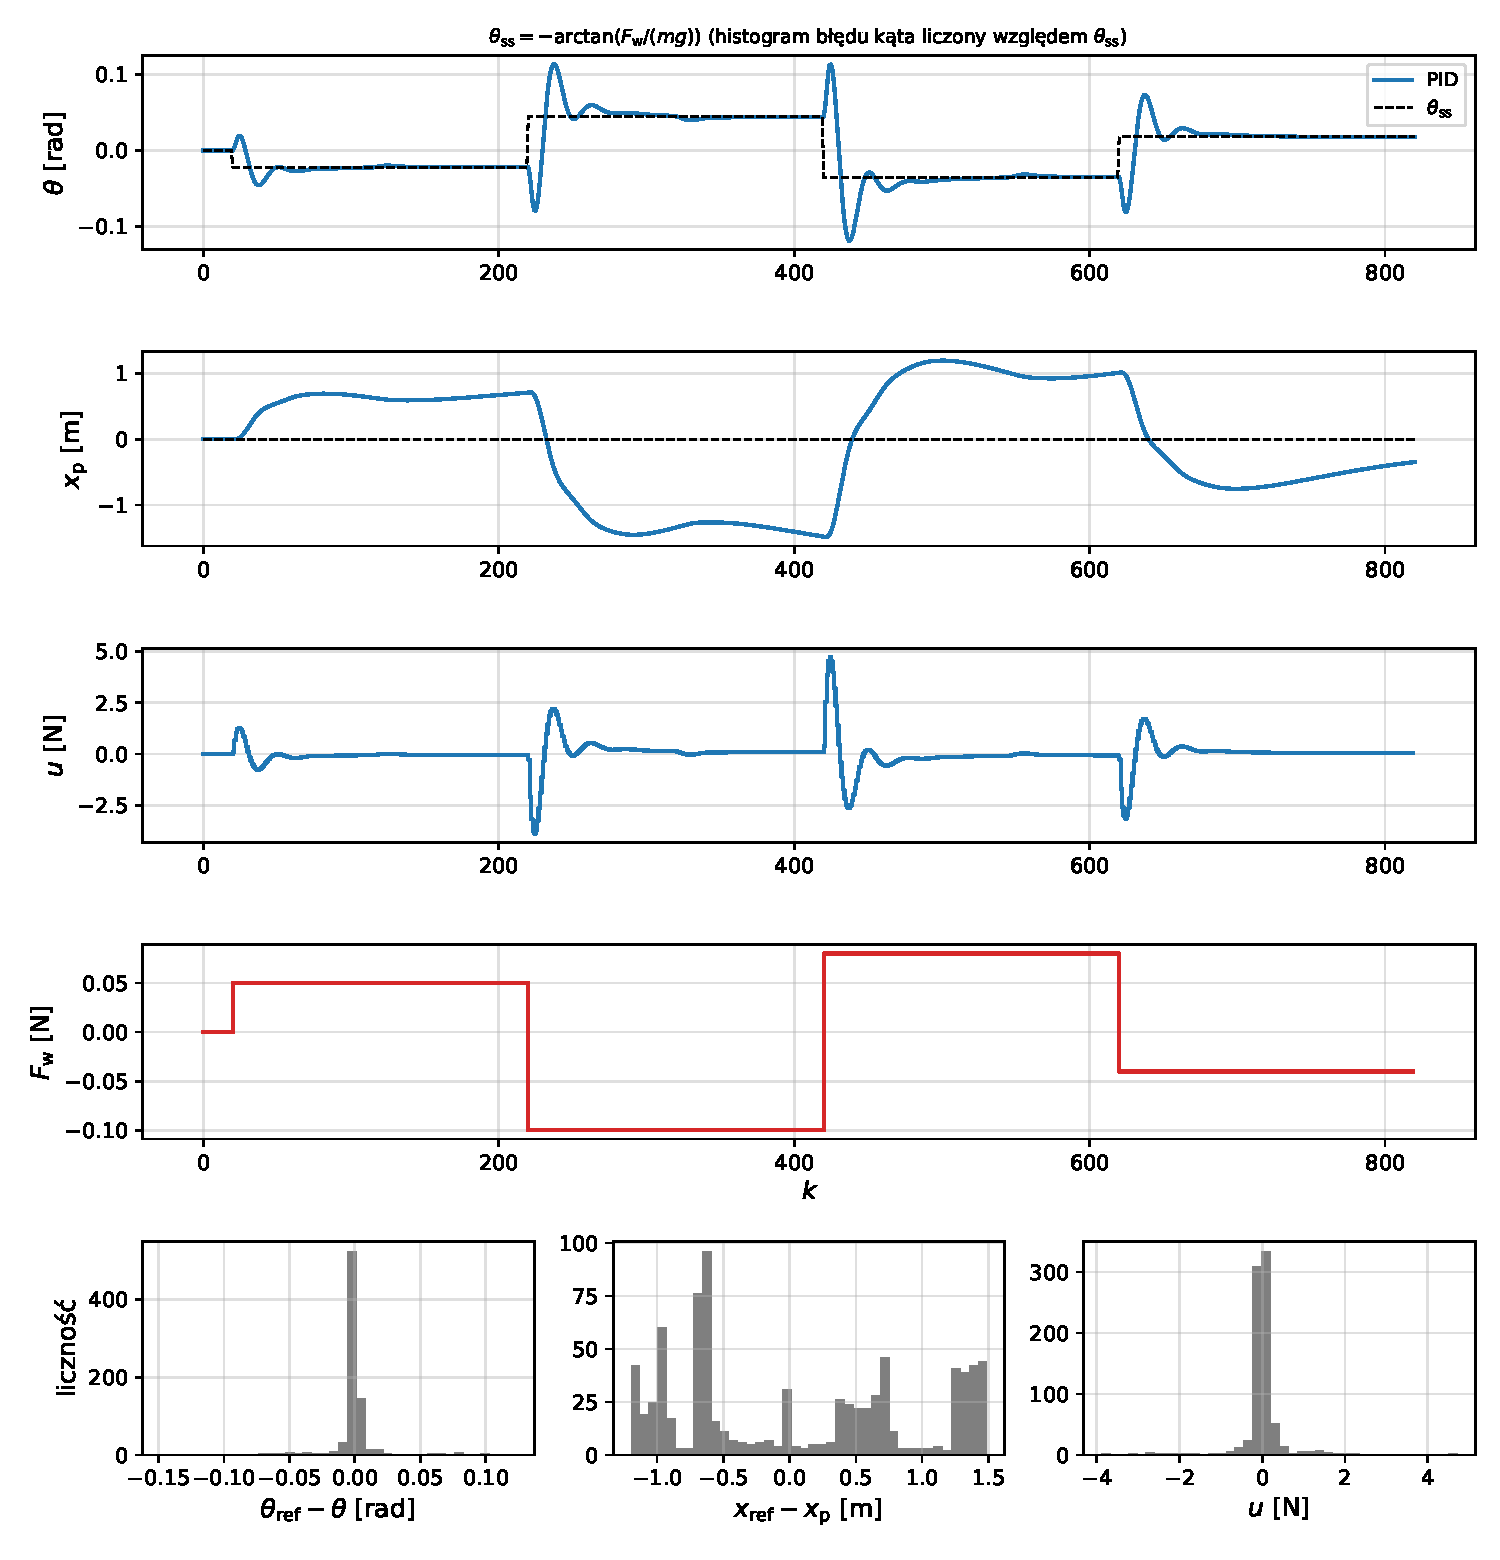
\includegraphics[width=\linewidth]{figs/S2_pid.pdf}
\caption{PID, Scenariusz S2 (skoki zakłócenia): status automatyczny -- \textbf{nieustalony}.}
\end{figure}
\clearpage
\begin{figure}[p]\centering
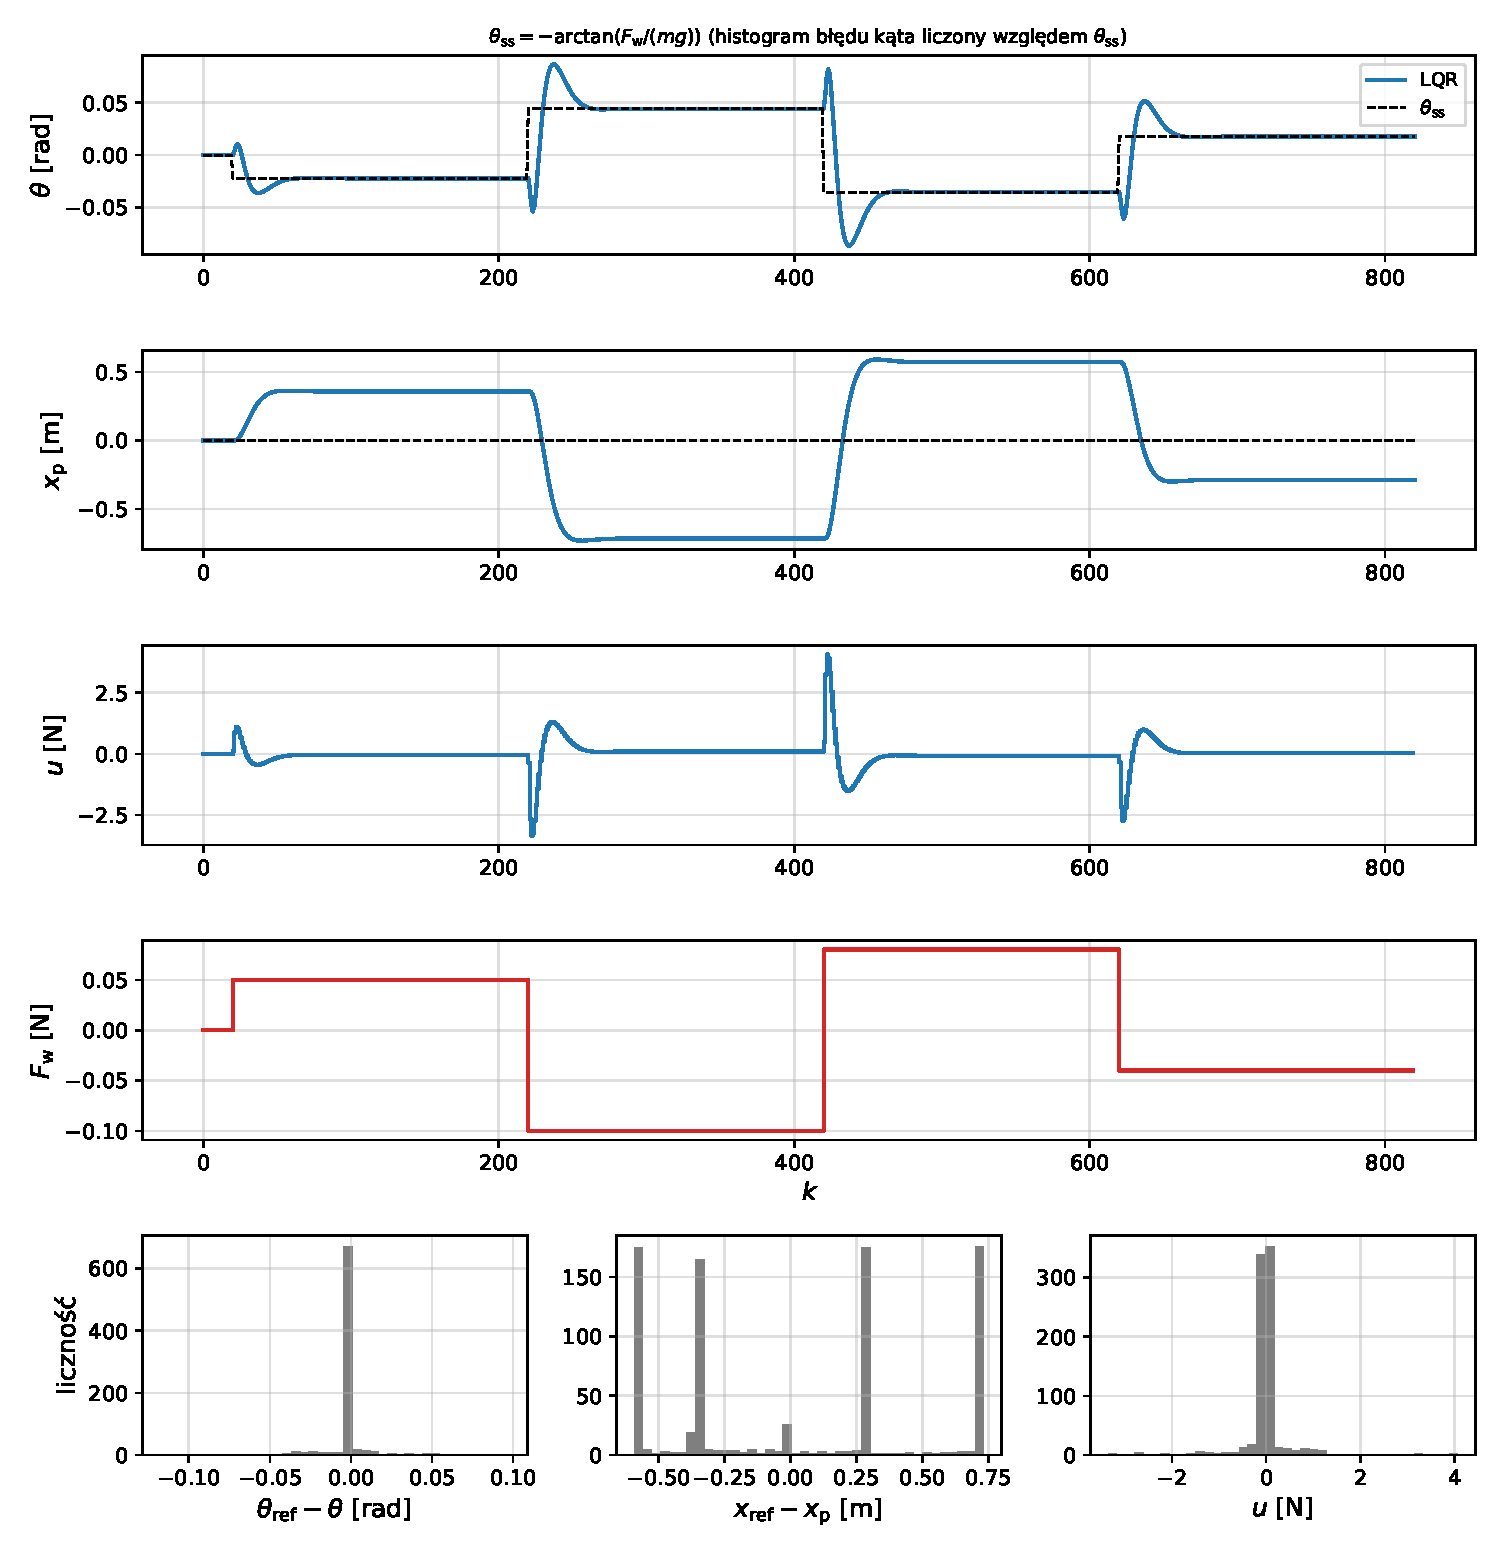
\includegraphics[width=\linewidth]{figs/S2_lqr.pdf}
\caption{LQR, Scenariusz S2 (skoki zakłócenia): status automatyczny -- stabilny.}
\end{figure}
\clearpage
\begin{figure}[p]\centering
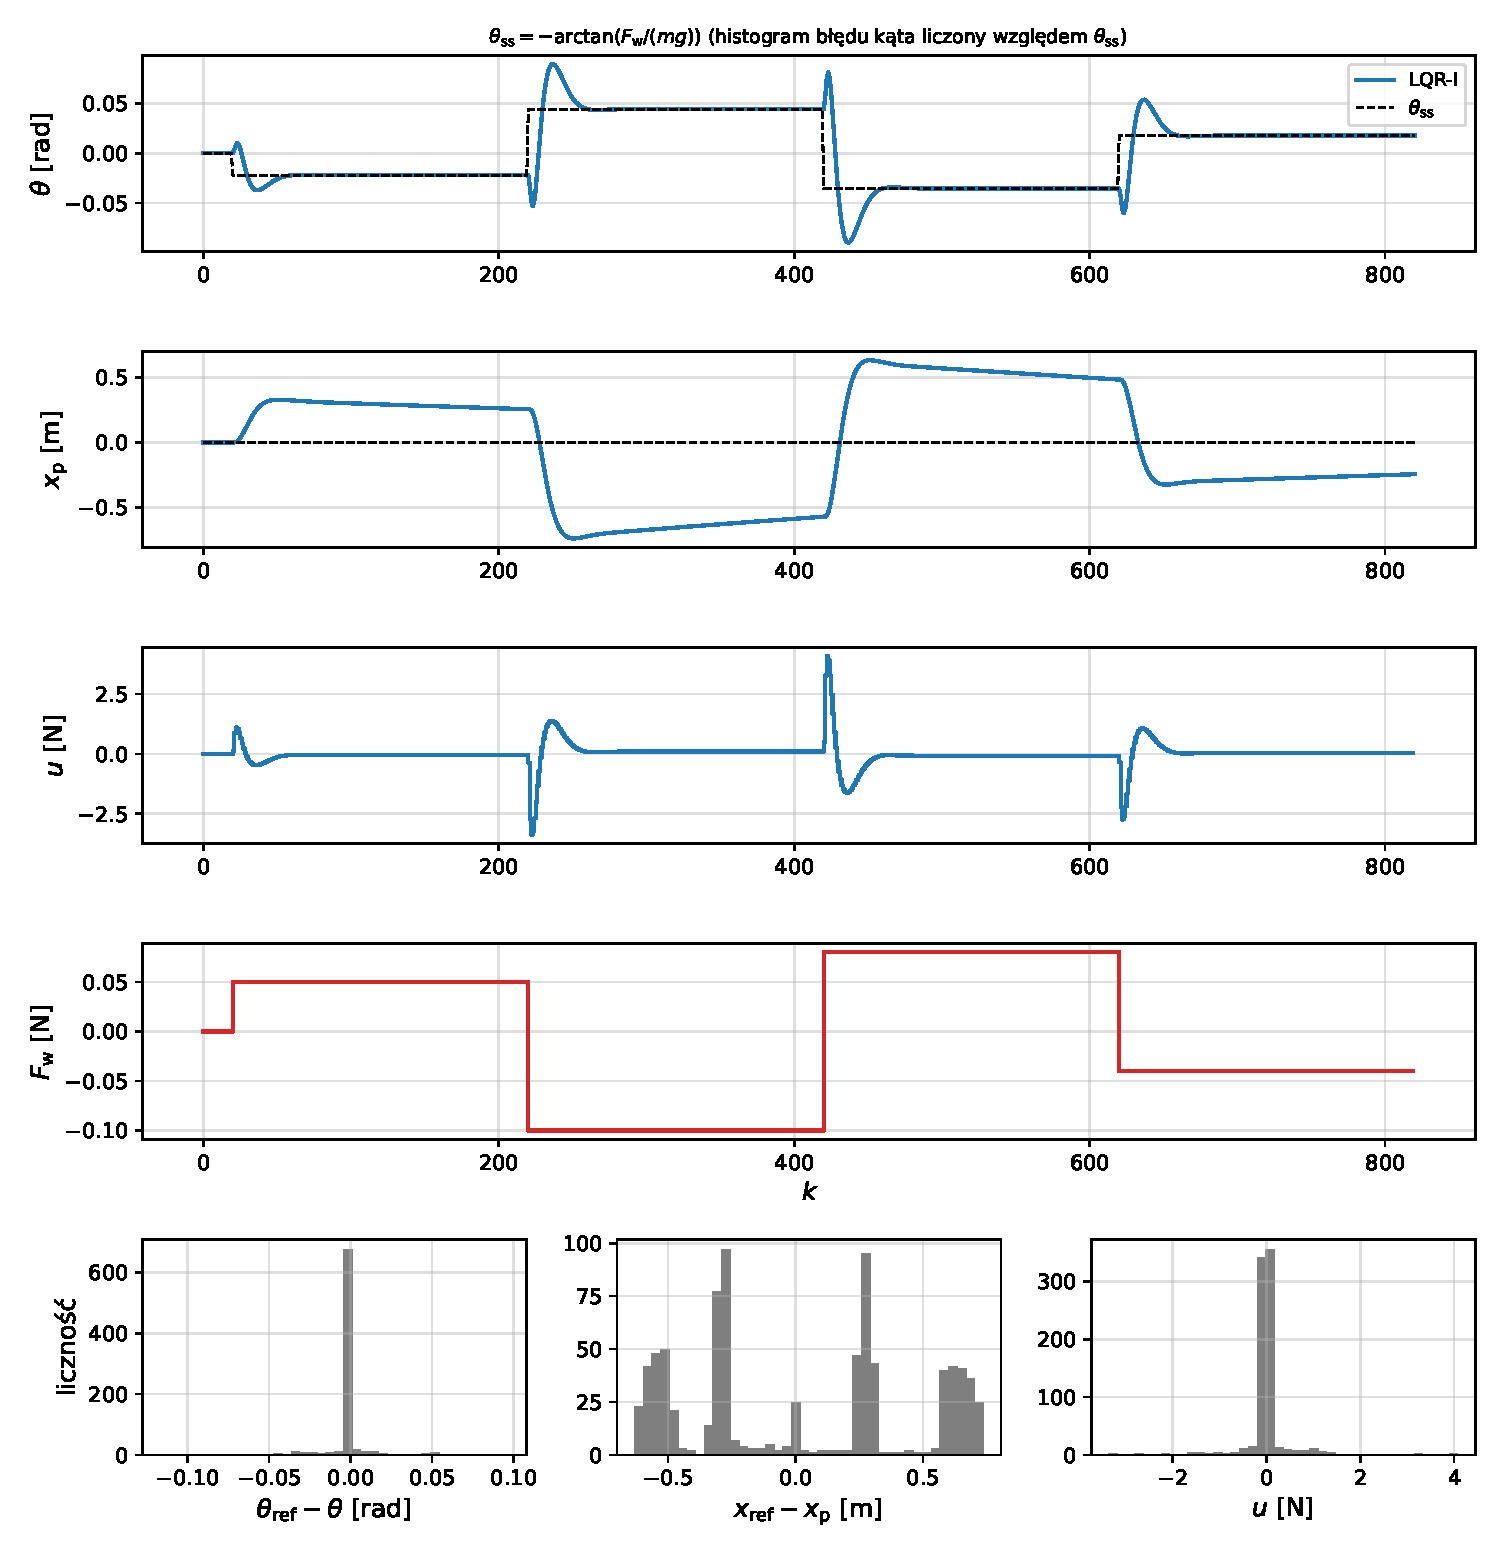
\includegraphics[width=\linewidth]{figs/S2_lqr_i.pdf}
\caption{LQR-I, Scenariusz S2 (skoki zakłócenia): status automatyczny -- stabilny.}
\end{figure}
\clearpage
\begin{figure}[p]\centering
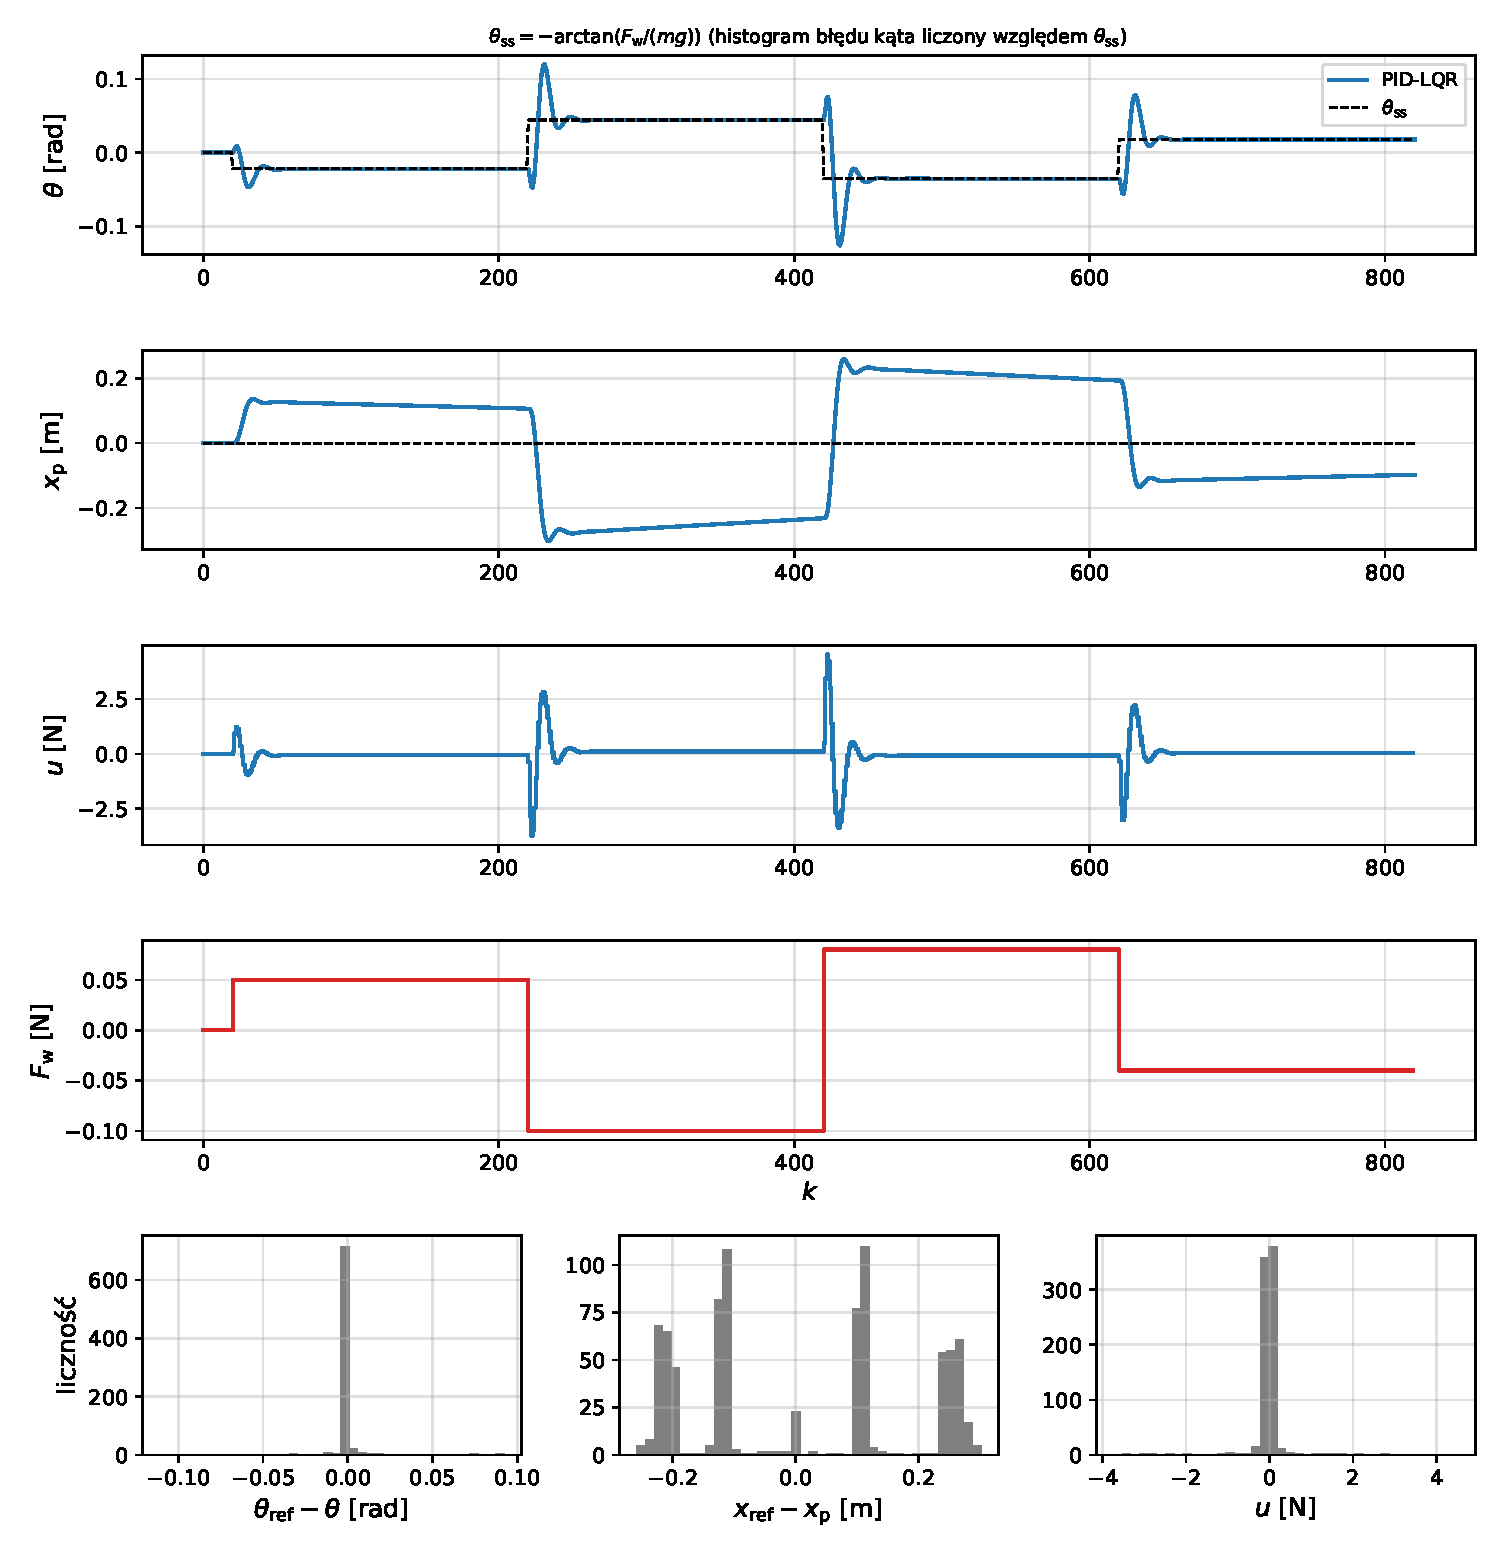
\includegraphics[width=\linewidth]{figs/S2_pid_lqr.pdf}
\caption{PID-LQR, Scenariusz S2 (skoki zakłócenia): status automatyczny -- stabilny.}
\end{figure}
\clearpage
\begin{figure}[p]\centering
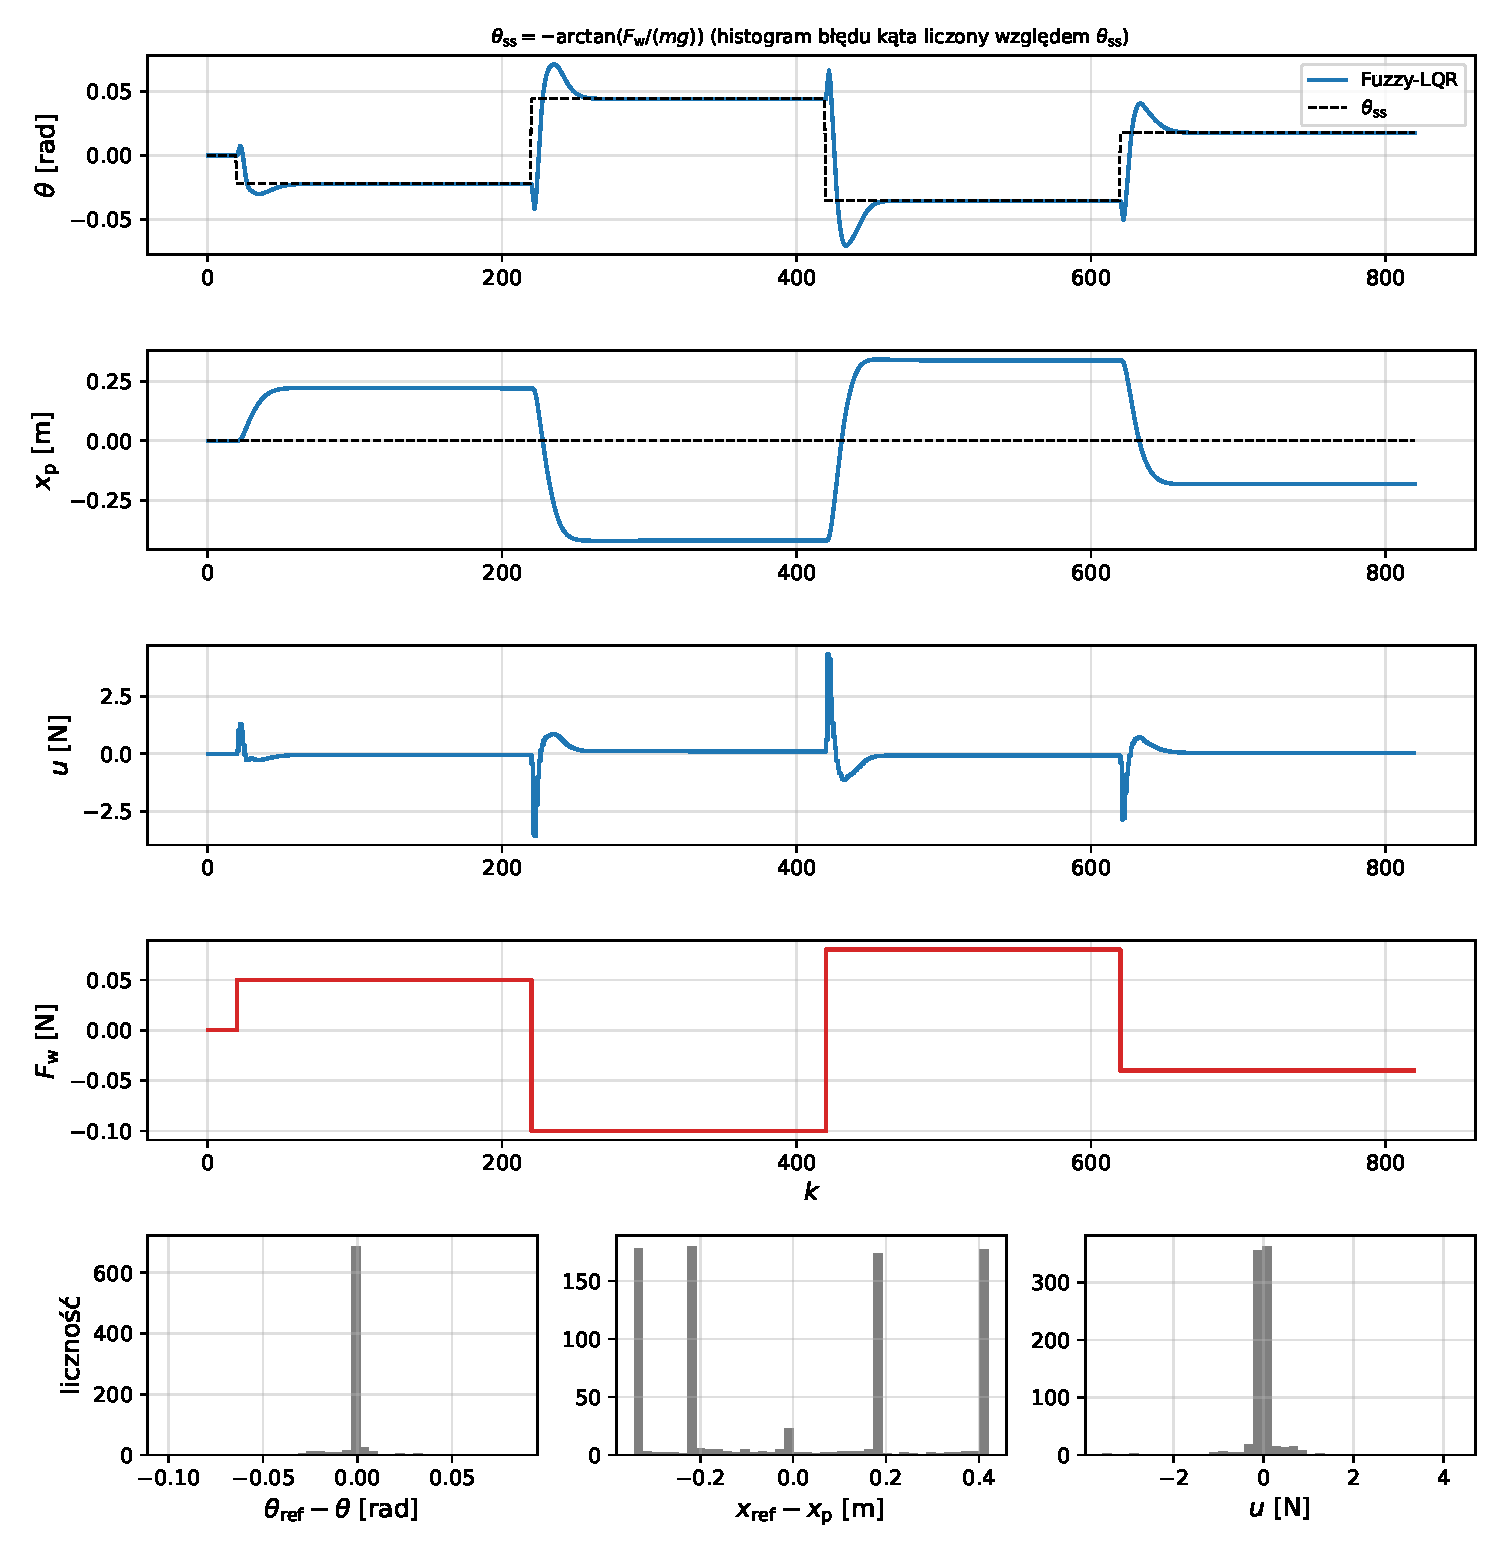
\includegraphics[width=\linewidth]{figs/S2_fuzzy_lqr.pdf}
\caption{Fuzzy-LQR, Scenariusz S2 (skoki zakłócenia): status automatyczny -- stabilny.}
\end{figure}
\clearpage
\begin{figure}[p]\centering
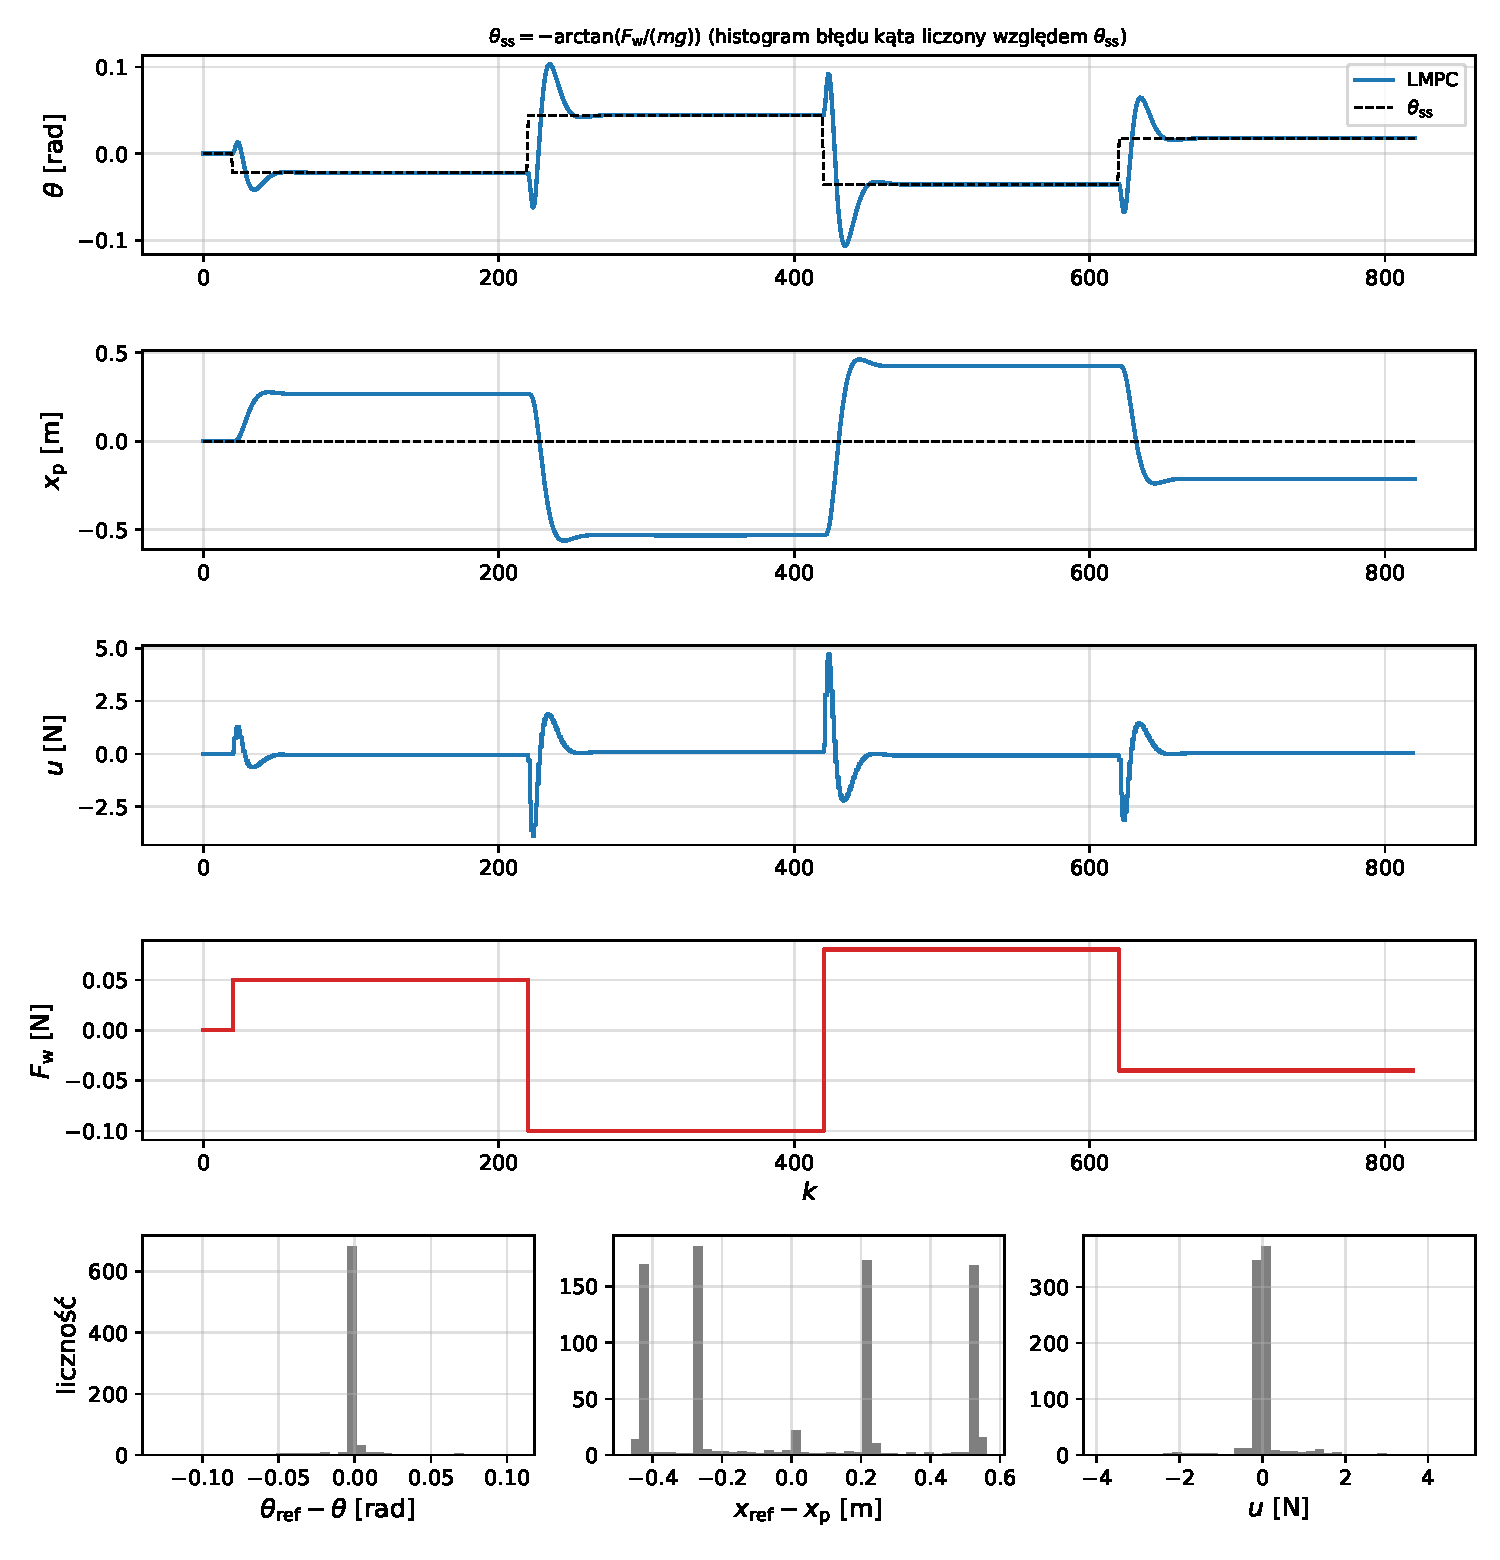
\includegraphics[width=\linewidth]{figs/S2_lmpc.pdf}
\caption{LMPC, Scenariusz S2 (skoki zakłócenia): status automatyczny -- stabilny.}
\end{figure}
\clearpage
\begin{figure}[p]\centering
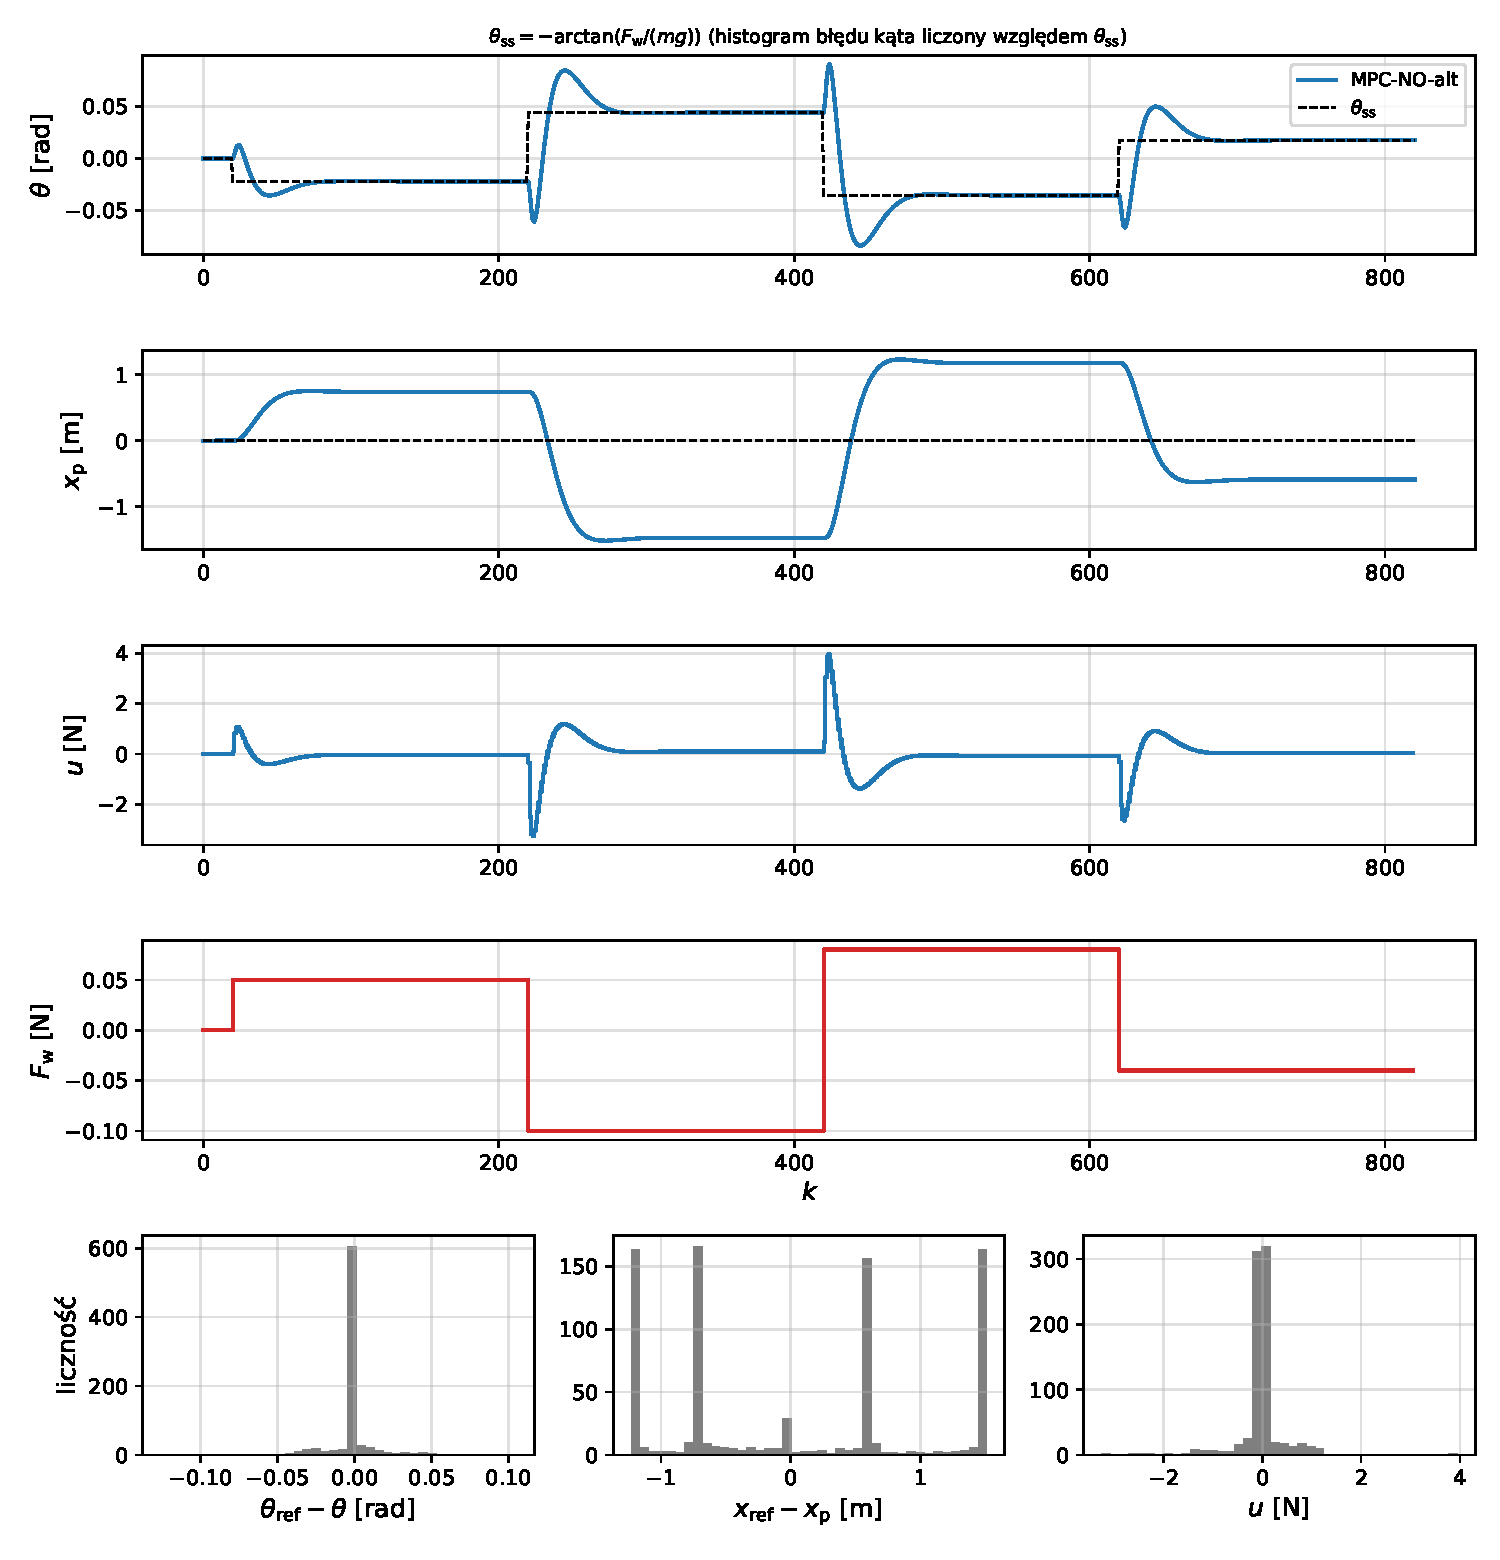
\includegraphics[width=\linewidth]{figs/S2_mpc_no_alt.pdf}
\caption{MPC-NO-alt, Scenariusz S2 (skoki zakłócenia): status automatyczny -- stabilny.}
\end{figure}
\clearpage
\begin{figure}[p]\centering
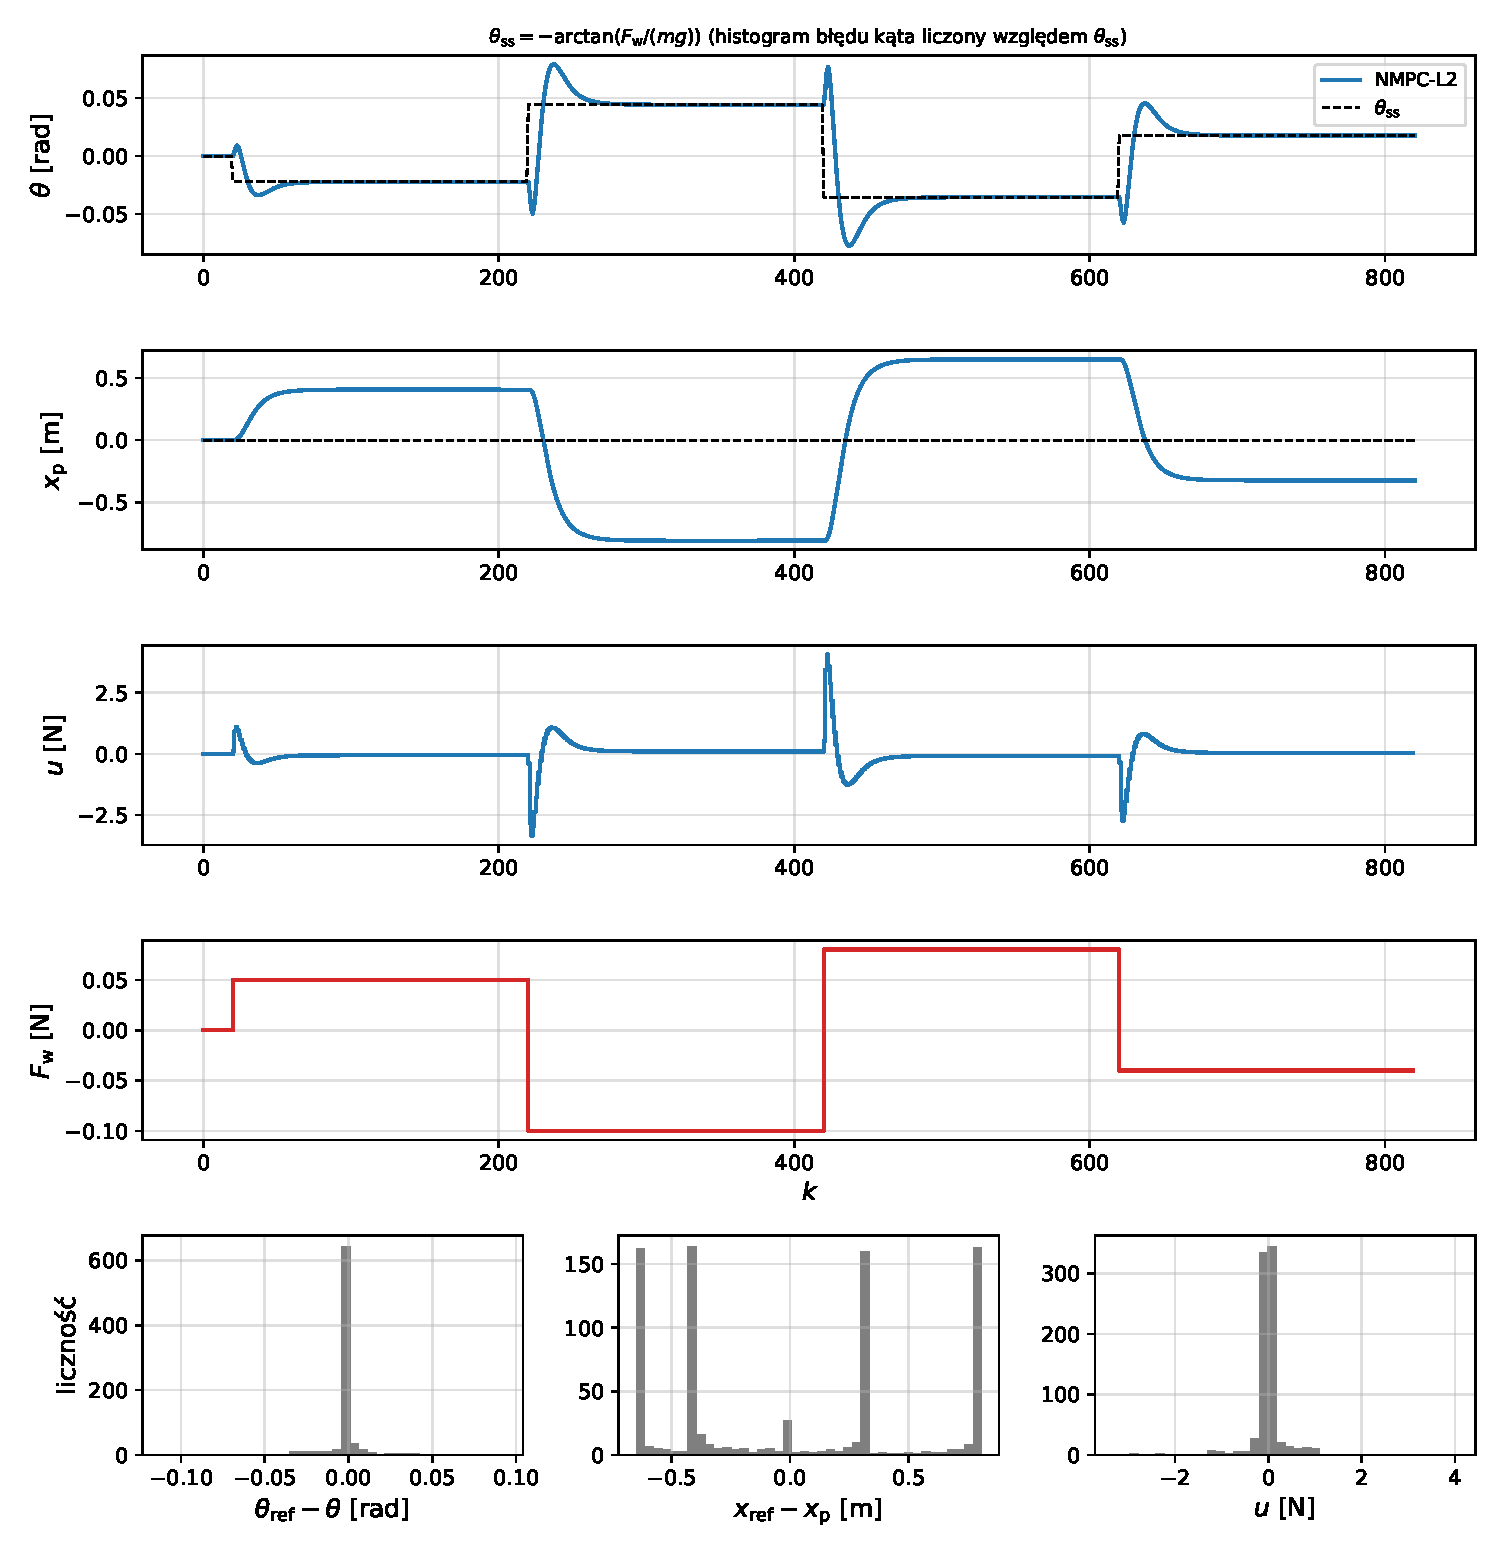
\includegraphics[width=\linewidth]{figs/S2_nmpc_l2.pdf}
\caption{NMPC-L$_2$, Scenariusz S2 (skoki zakłócenia): status automatyczny -- stabilny.}
\end{figure}
\clearpage
\begin{figure}[p]\centering
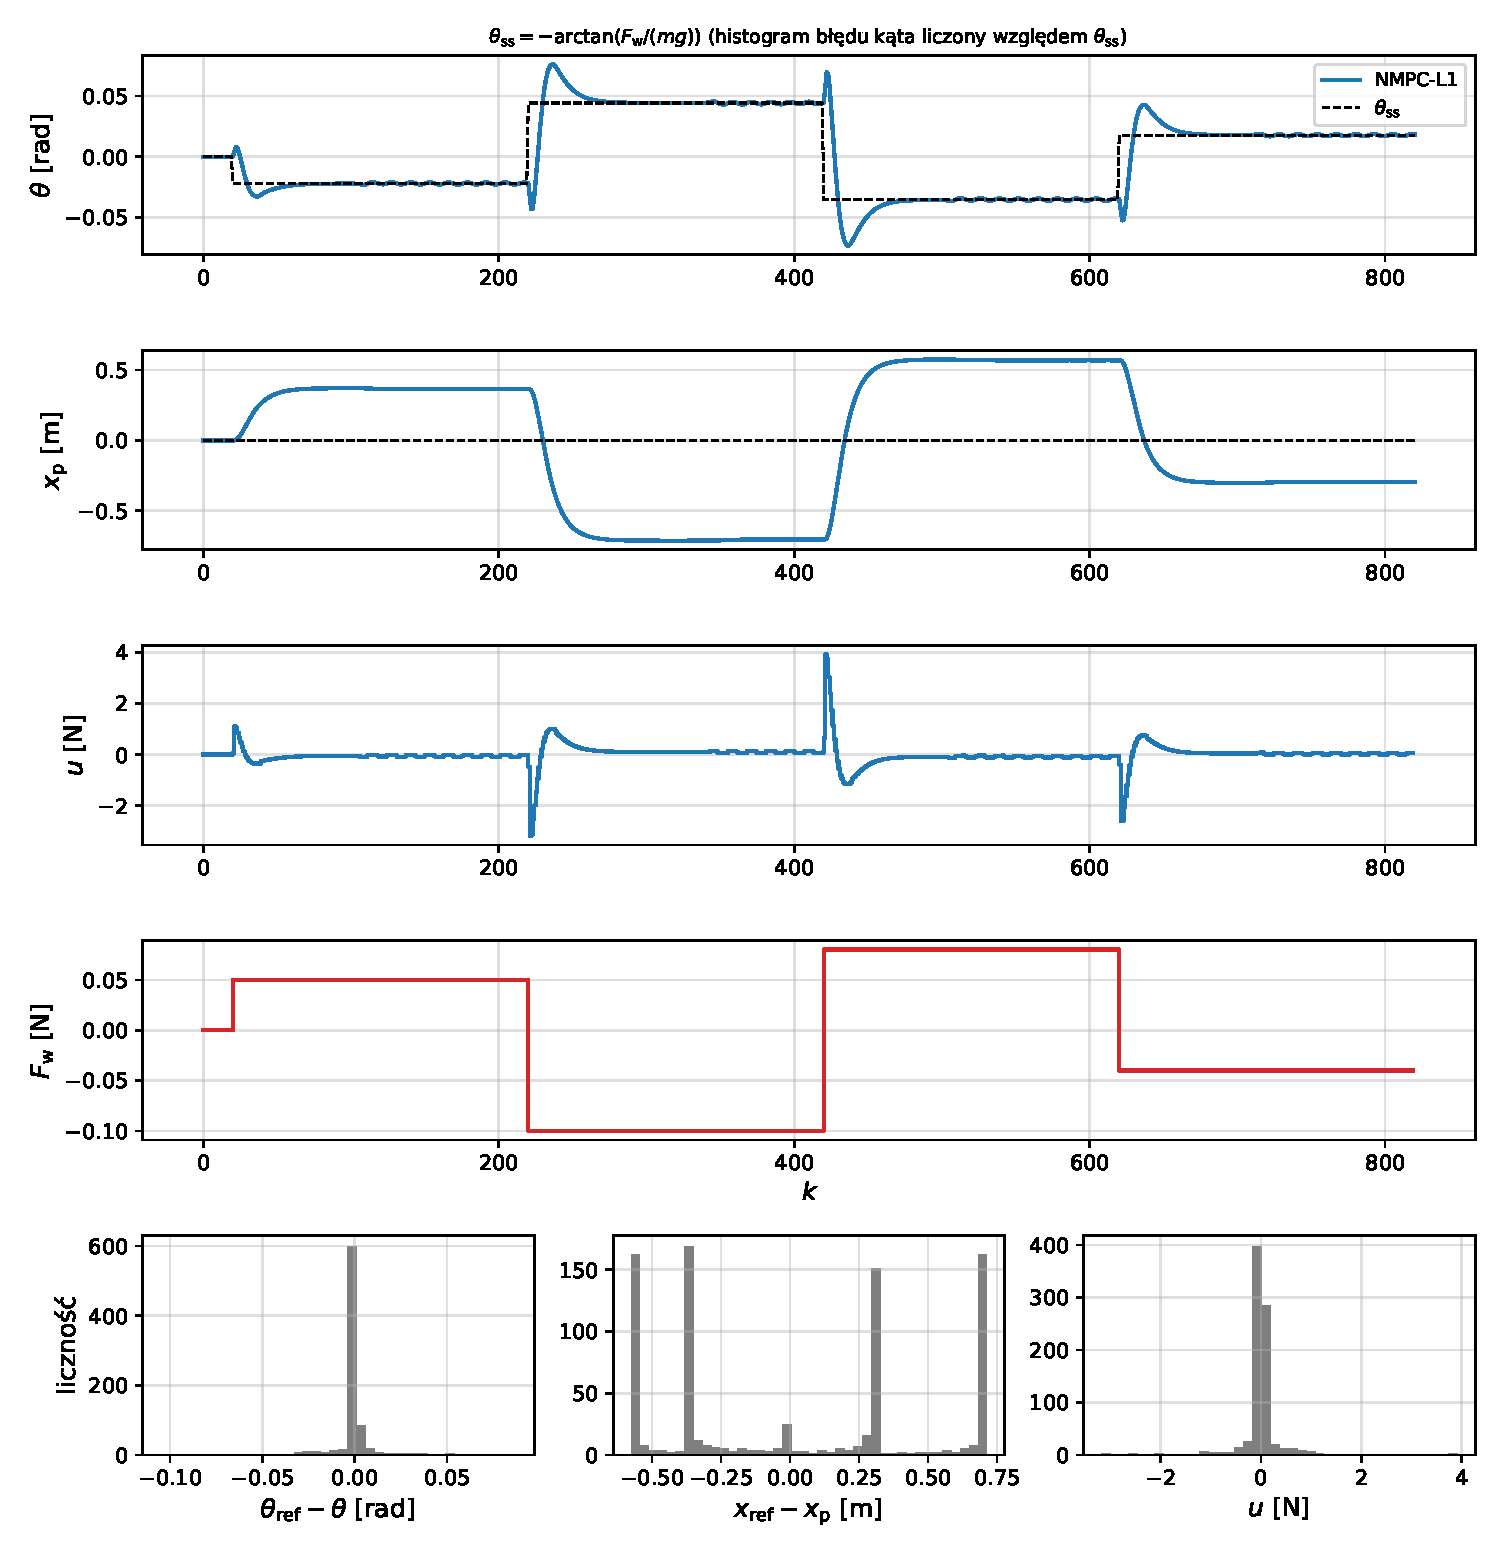
\includegraphics[width=\linewidth]{figs/S2_nmpc_l1.pdf}
\caption{NMPC-L$_1$, Scenariusz S2 (skoki zakłócenia): status automatyczny -- stabilny.}
\end{figure}
\clearpage
\begin{figure}[p]\centering
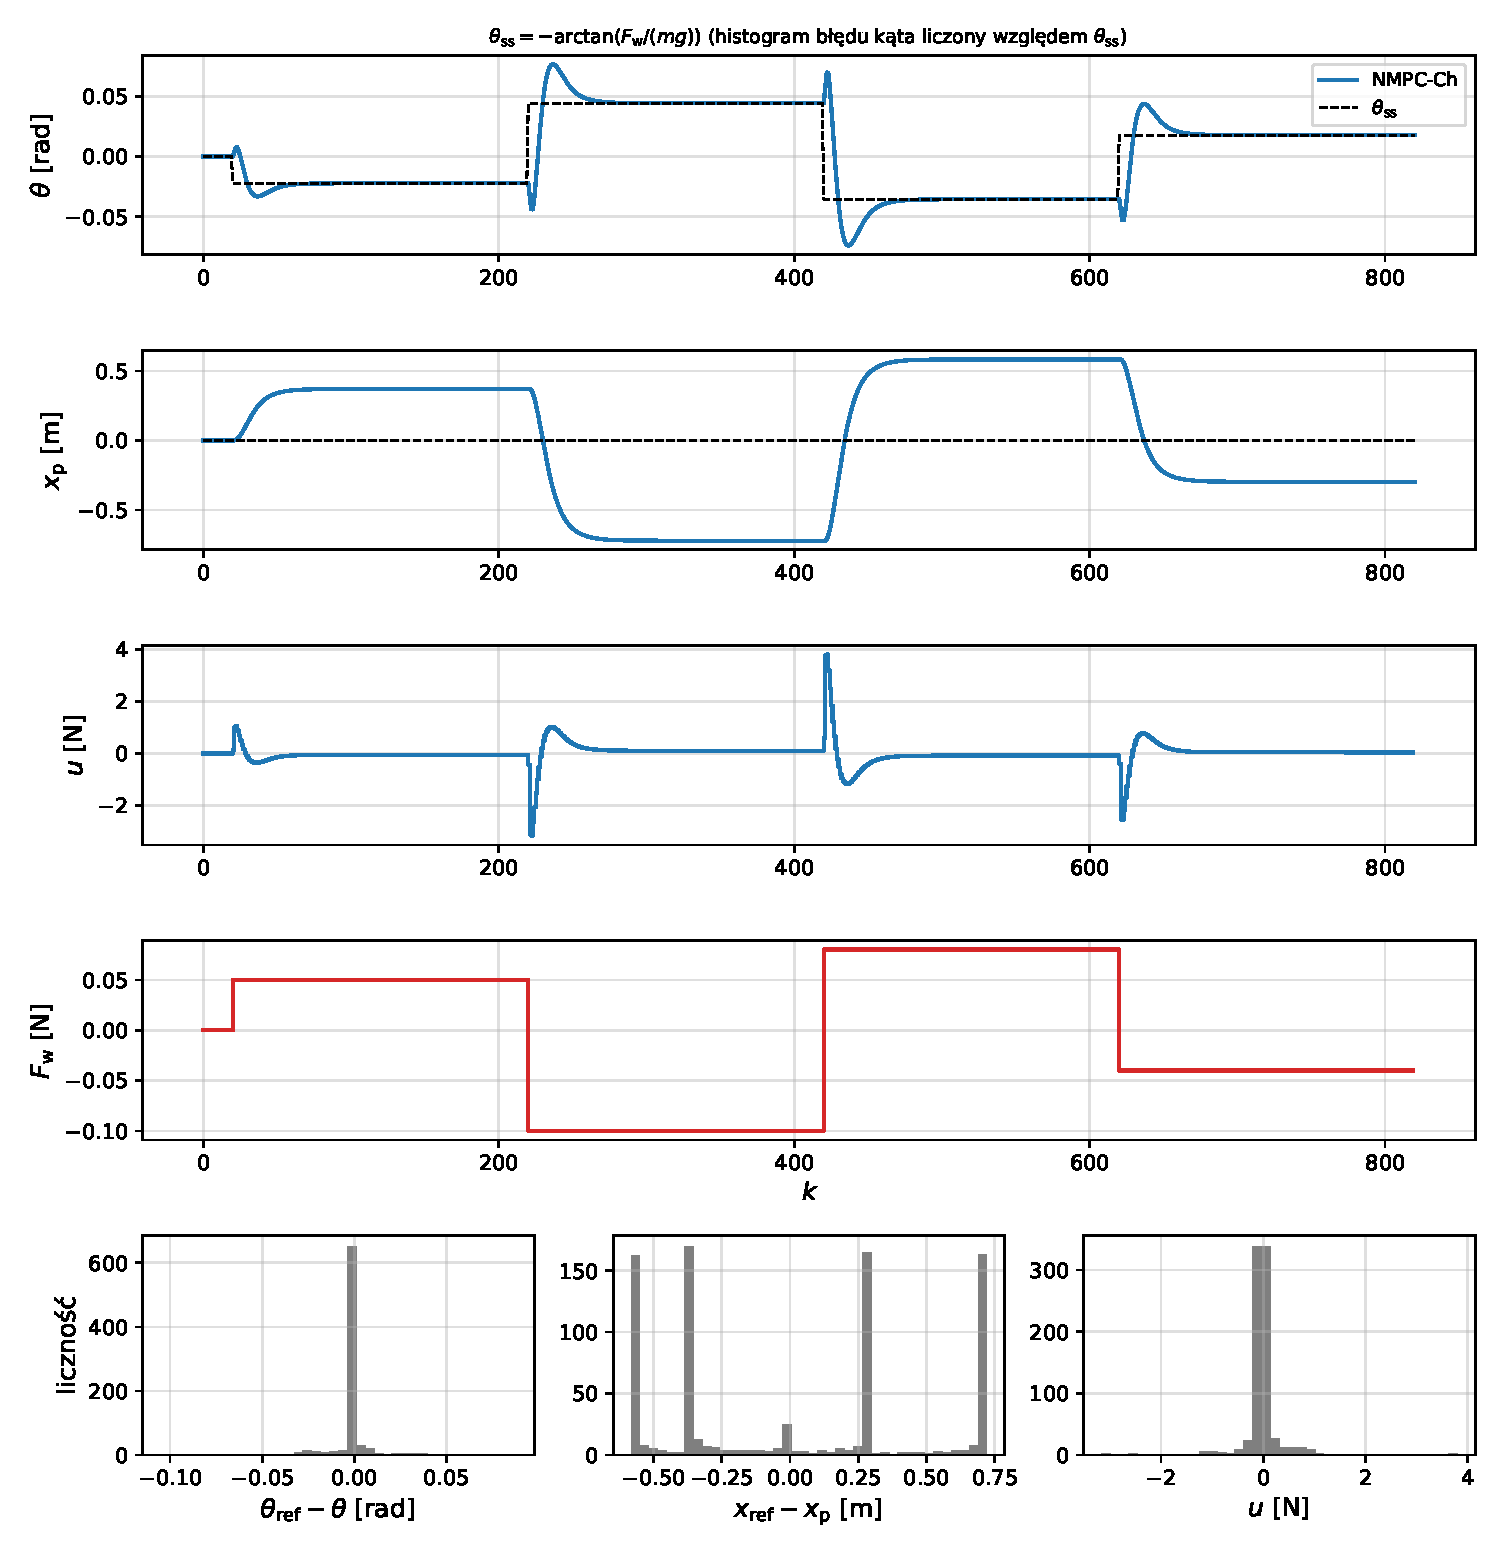
\includegraphics[width=\linewidth]{figs/S2_nmpc_ch.pdf}
\caption{NMPC-Ch, Scenariusz S2 (skoki zakłócenia): status automatyczny -- stabilny.}
\end{figure}
\clearpage
\begin{figure}[p]\centering
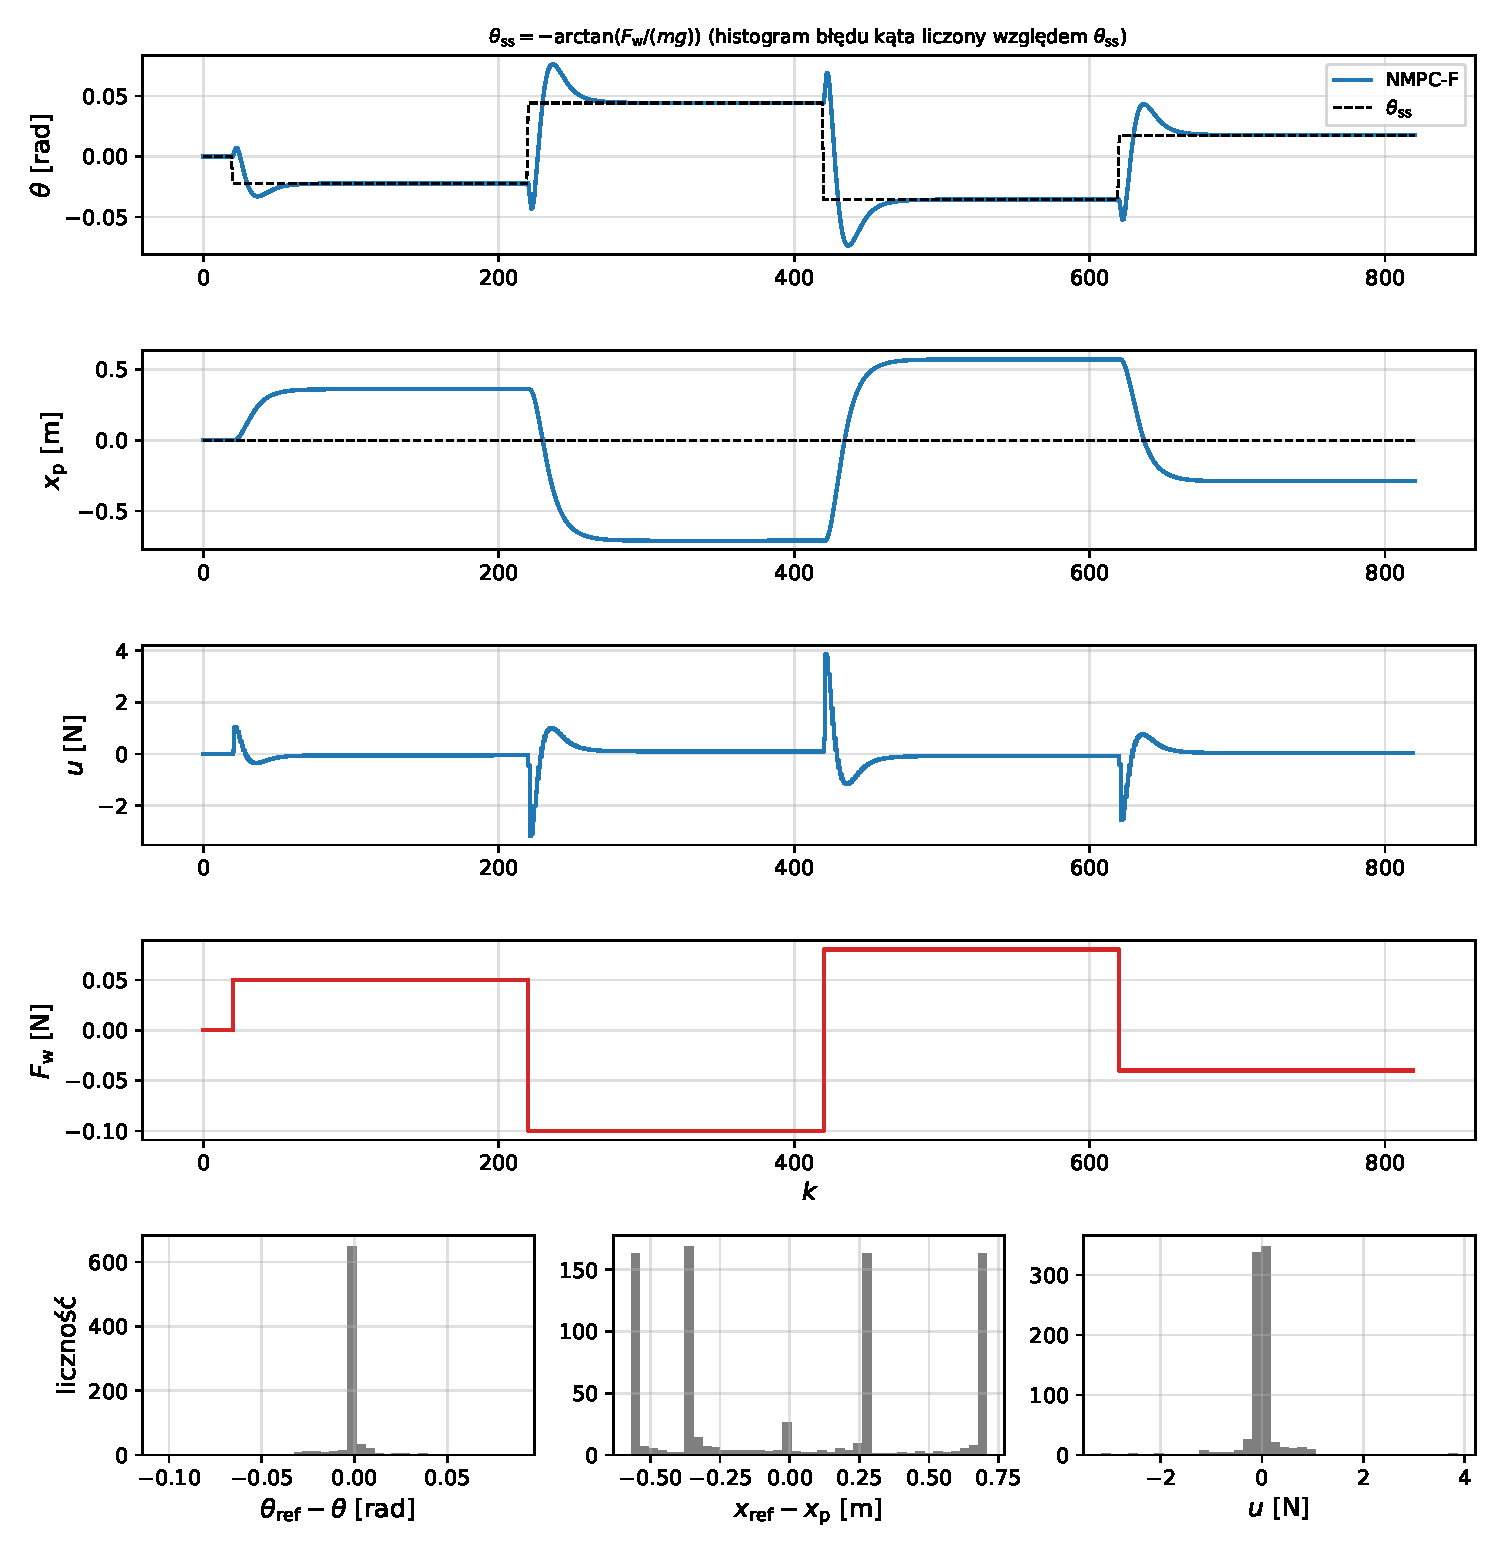
\includegraphics[width=\linewidth]{figs/S2_nmpc_f.pdf}
\caption{NMPC-F, Scenariusz S2 (skoki zakłócenia): status automatyczny -- stabilny.}
\end{figure}
\clearpage
\begin{figure}[p]\centering
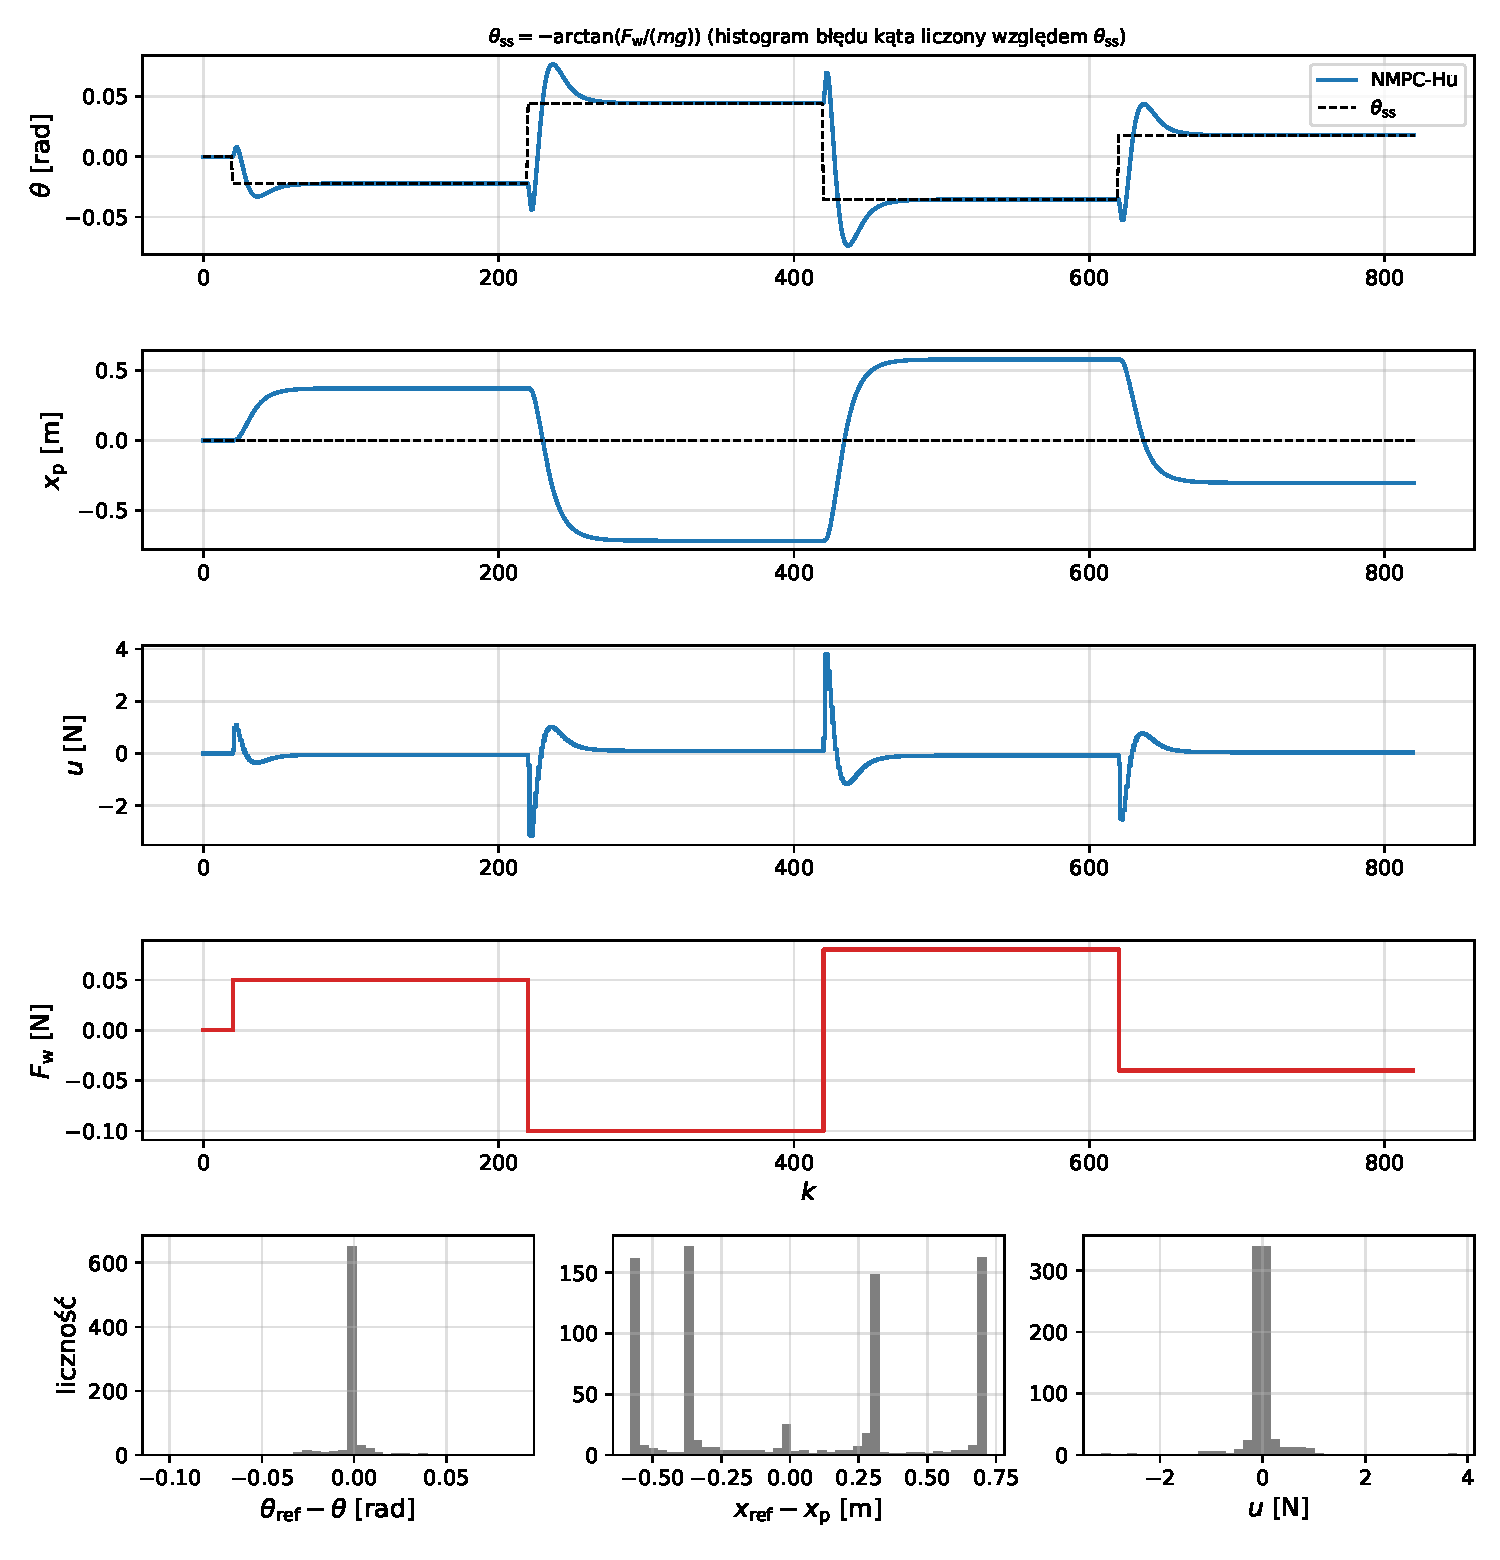
\includegraphics[width=\linewidth]{figs/S2_nmpc_hu.pdf}
\caption{NMPC-Hu, Scenariusz S2 (skoki zakłócenia): status automatyczny -- stabilny.}
\end{figure}
\clearpage
\begin{figure}[p]\centering
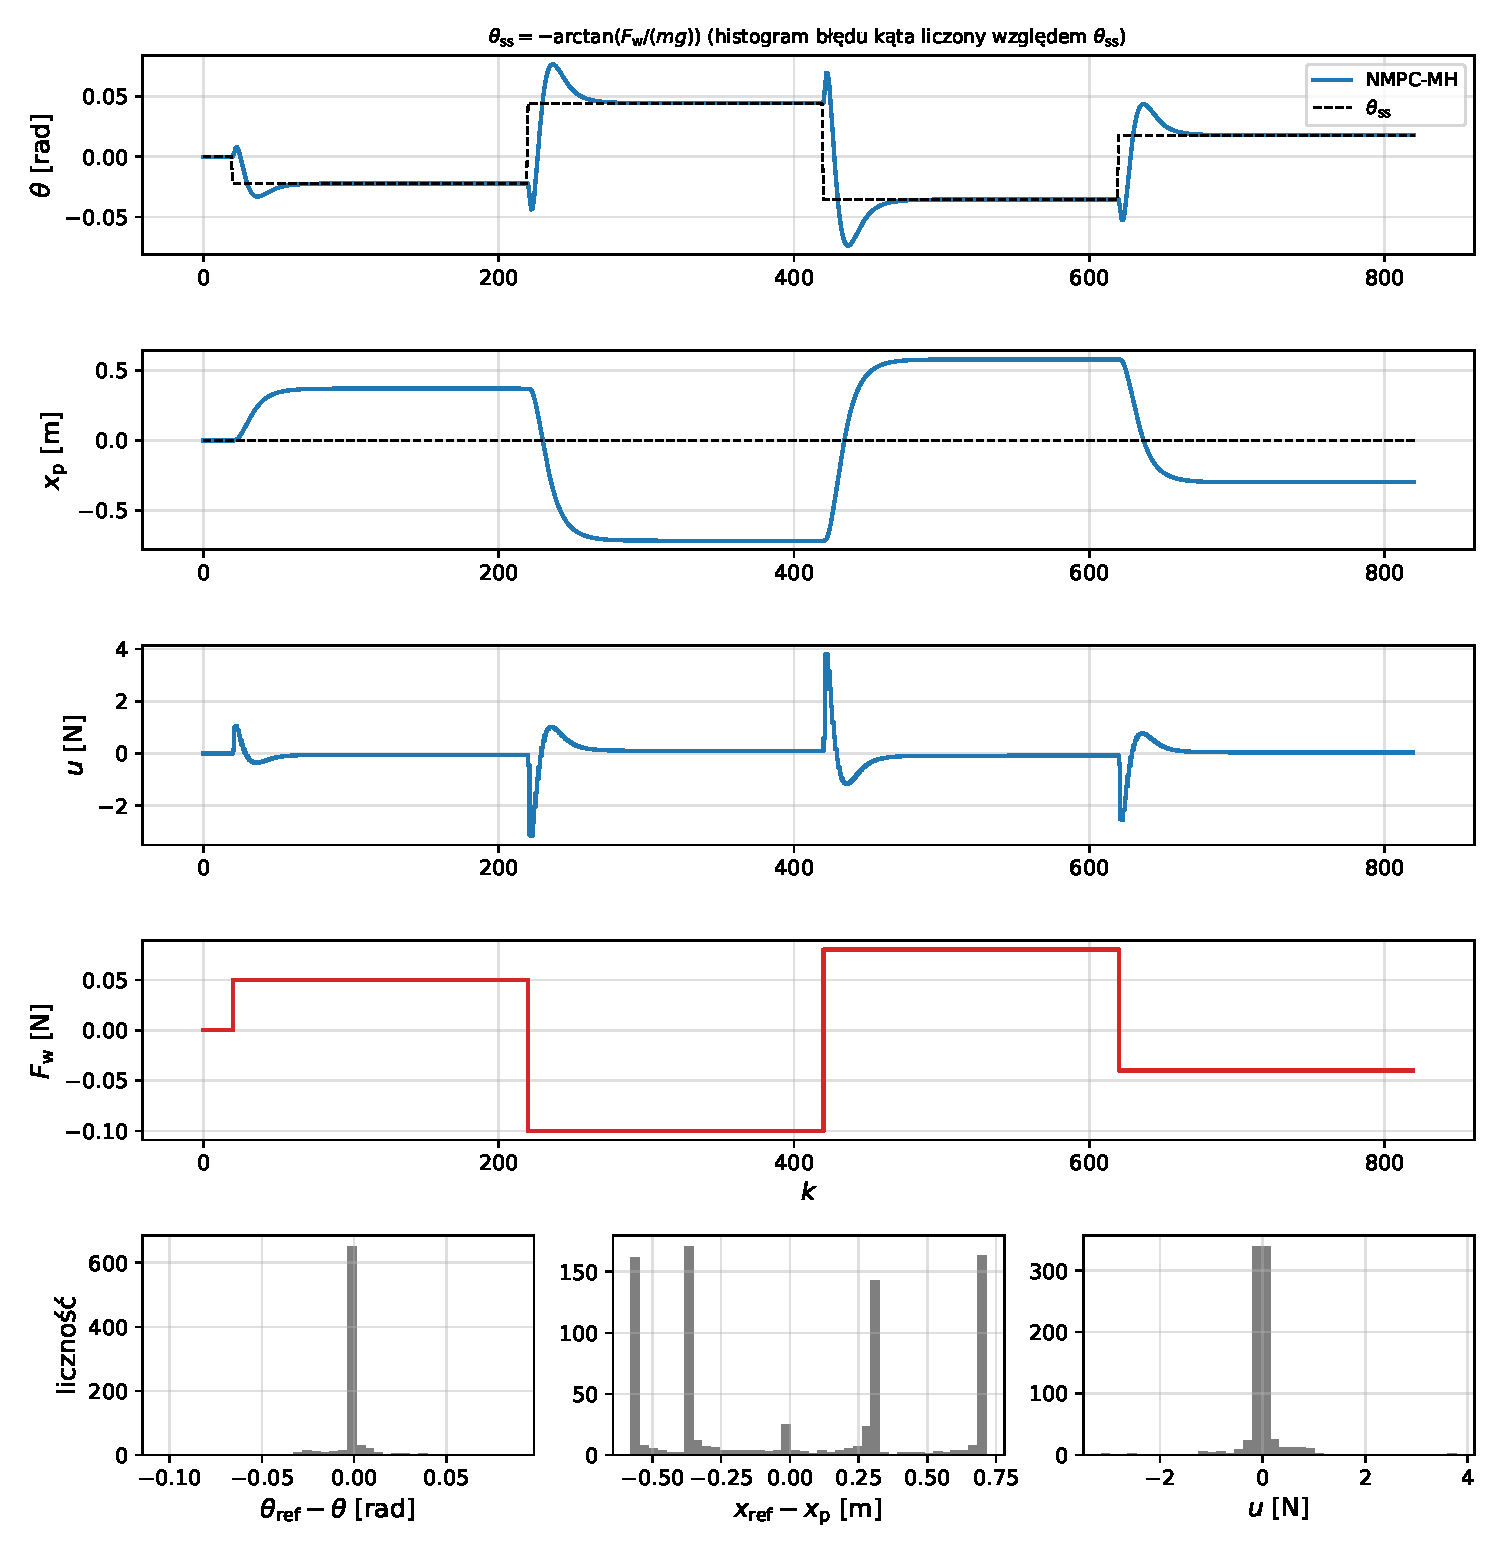
\includegraphics[width=\linewidth]{figs/S2_nmpc_mh.pdf}
\caption{NMPC-MH, Scenariusz S2 (skoki zakłócenia): status automatyczny -- stabilny.}
\end{figure}
\clearpage
\begin{figure}[p]\centering
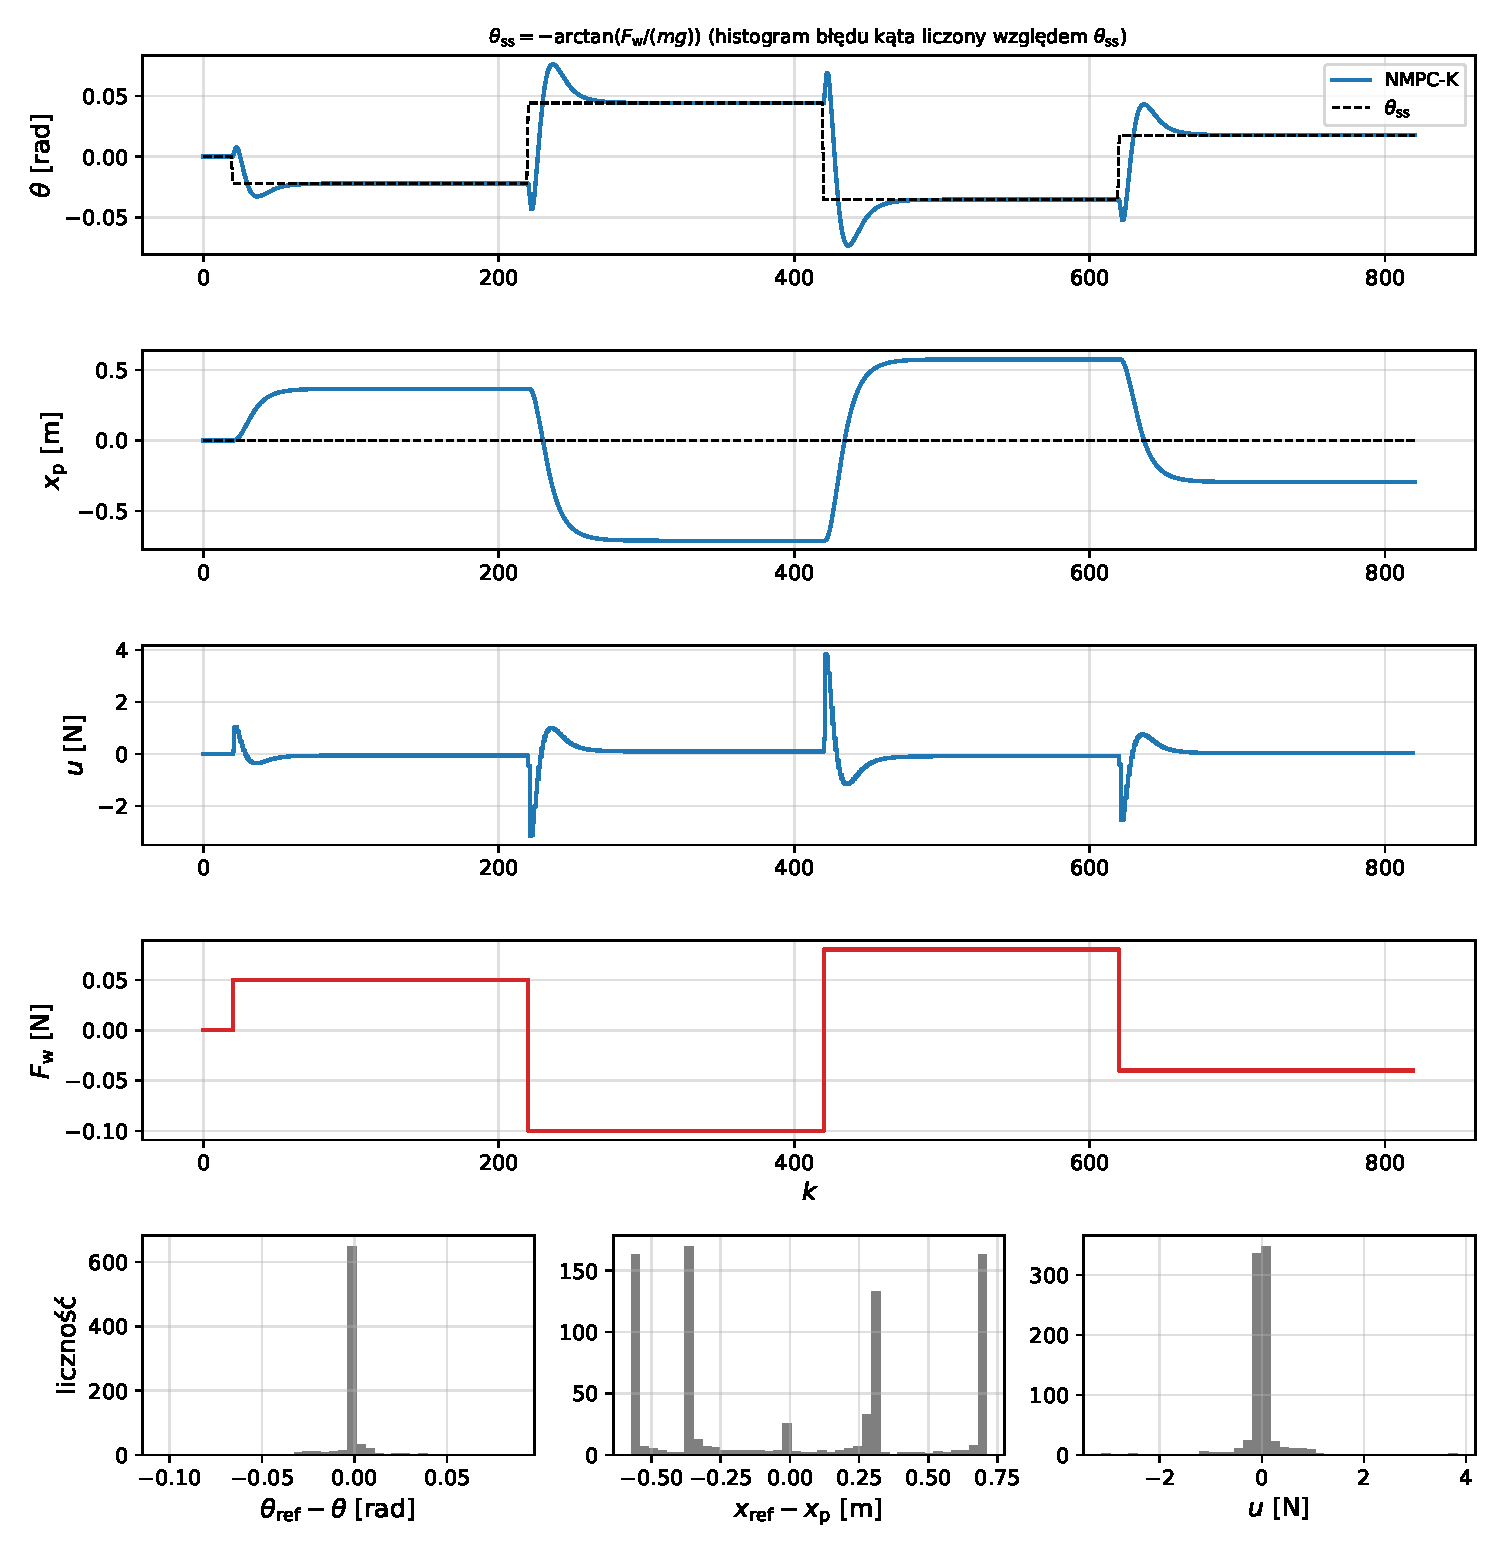
\includegraphics[width=\linewidth]{figs/S2_nmpc_k.pdf}
\caption{NMPC-K, Scenariusz S2 (skoki zakłócenia): status automatyczny -- stabilny.}
\end{figure}
\clearpage
\begin{figure}[p]\centering
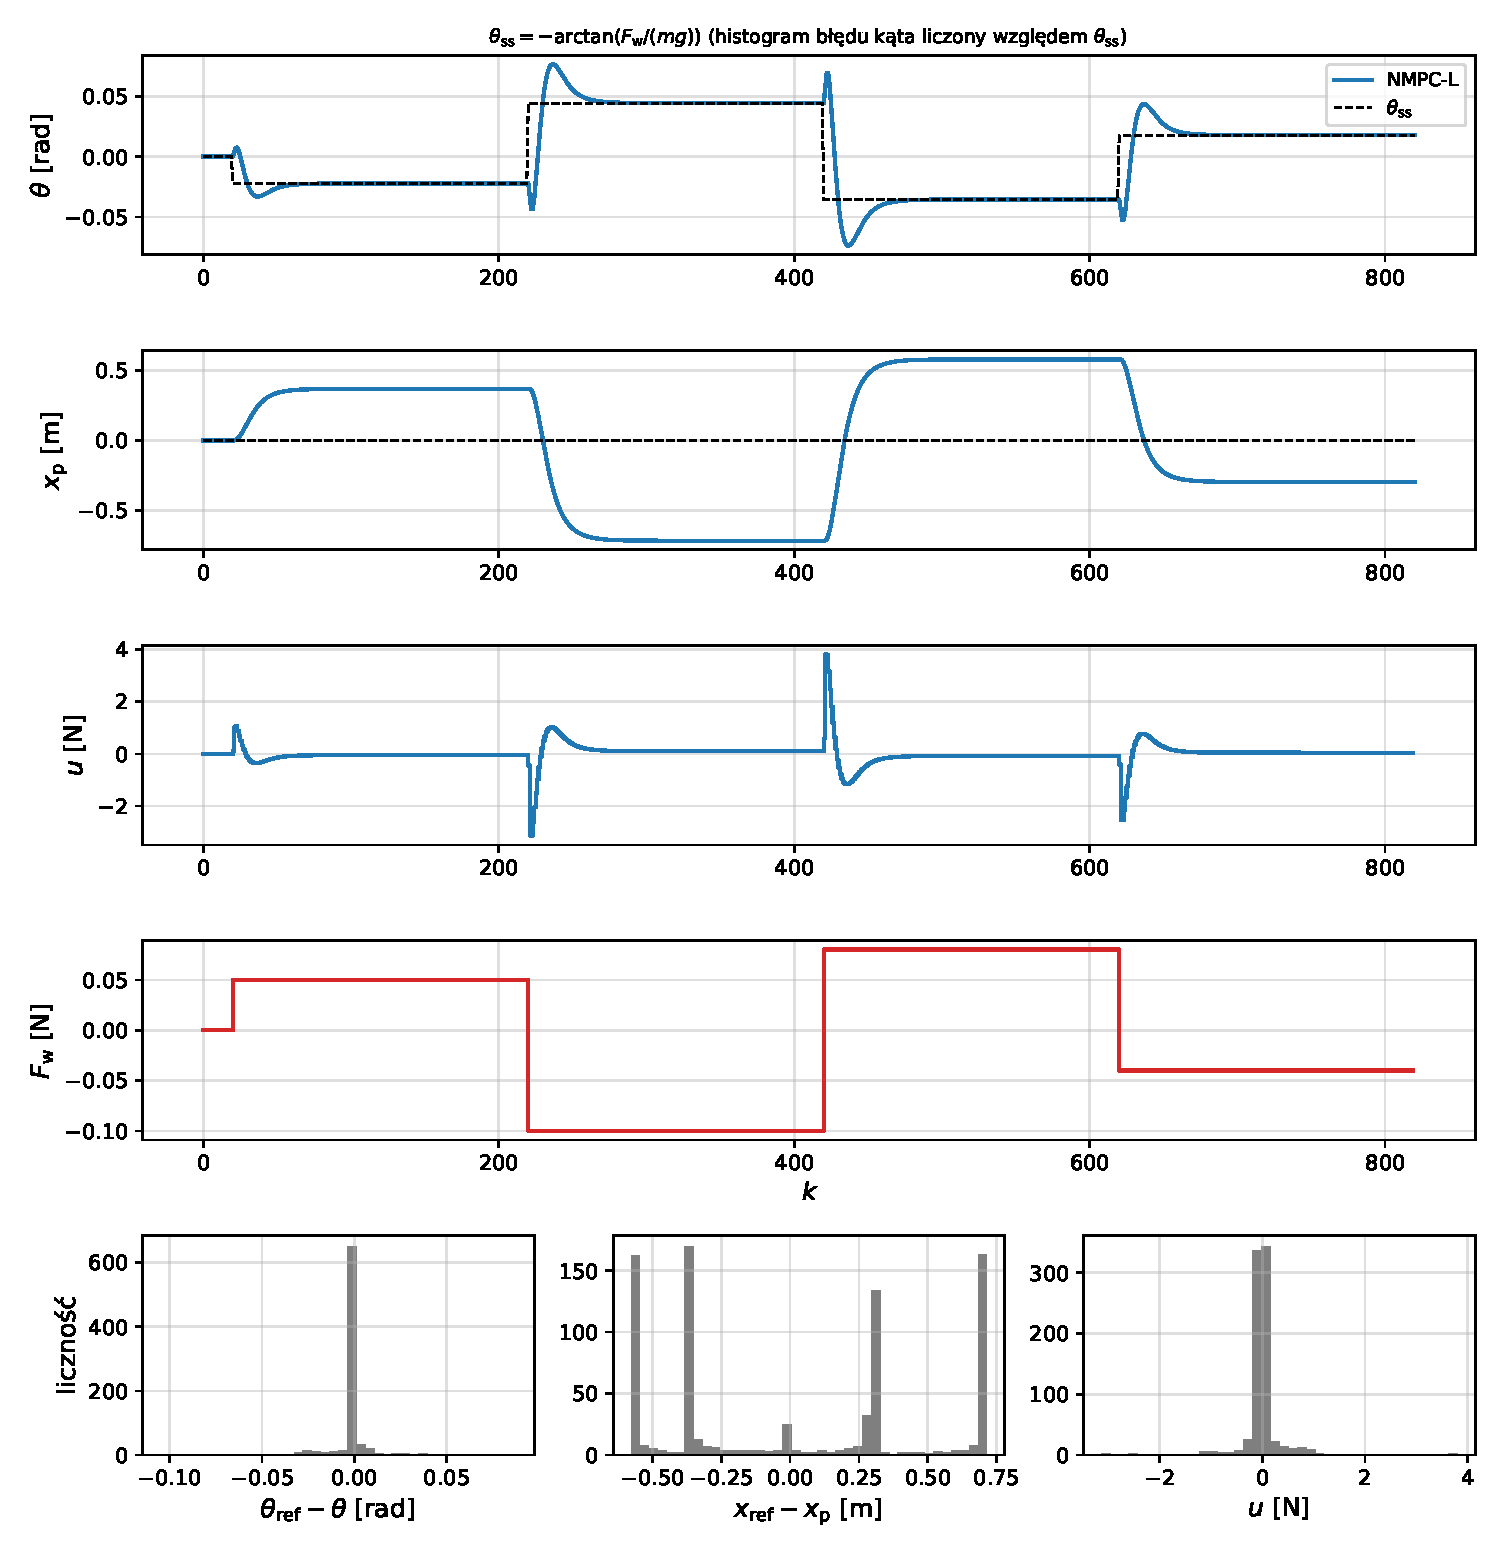
\includegraphics[width=\linewidth]{figs/S2_nmpc_l.pdf}
\caption{NMPC-L, Scenariusz S2 (skoki zakłócenia): status automatyczny -- stabilny.}
\end{figure}
\clearpage
\begin{figure}[p]\centering
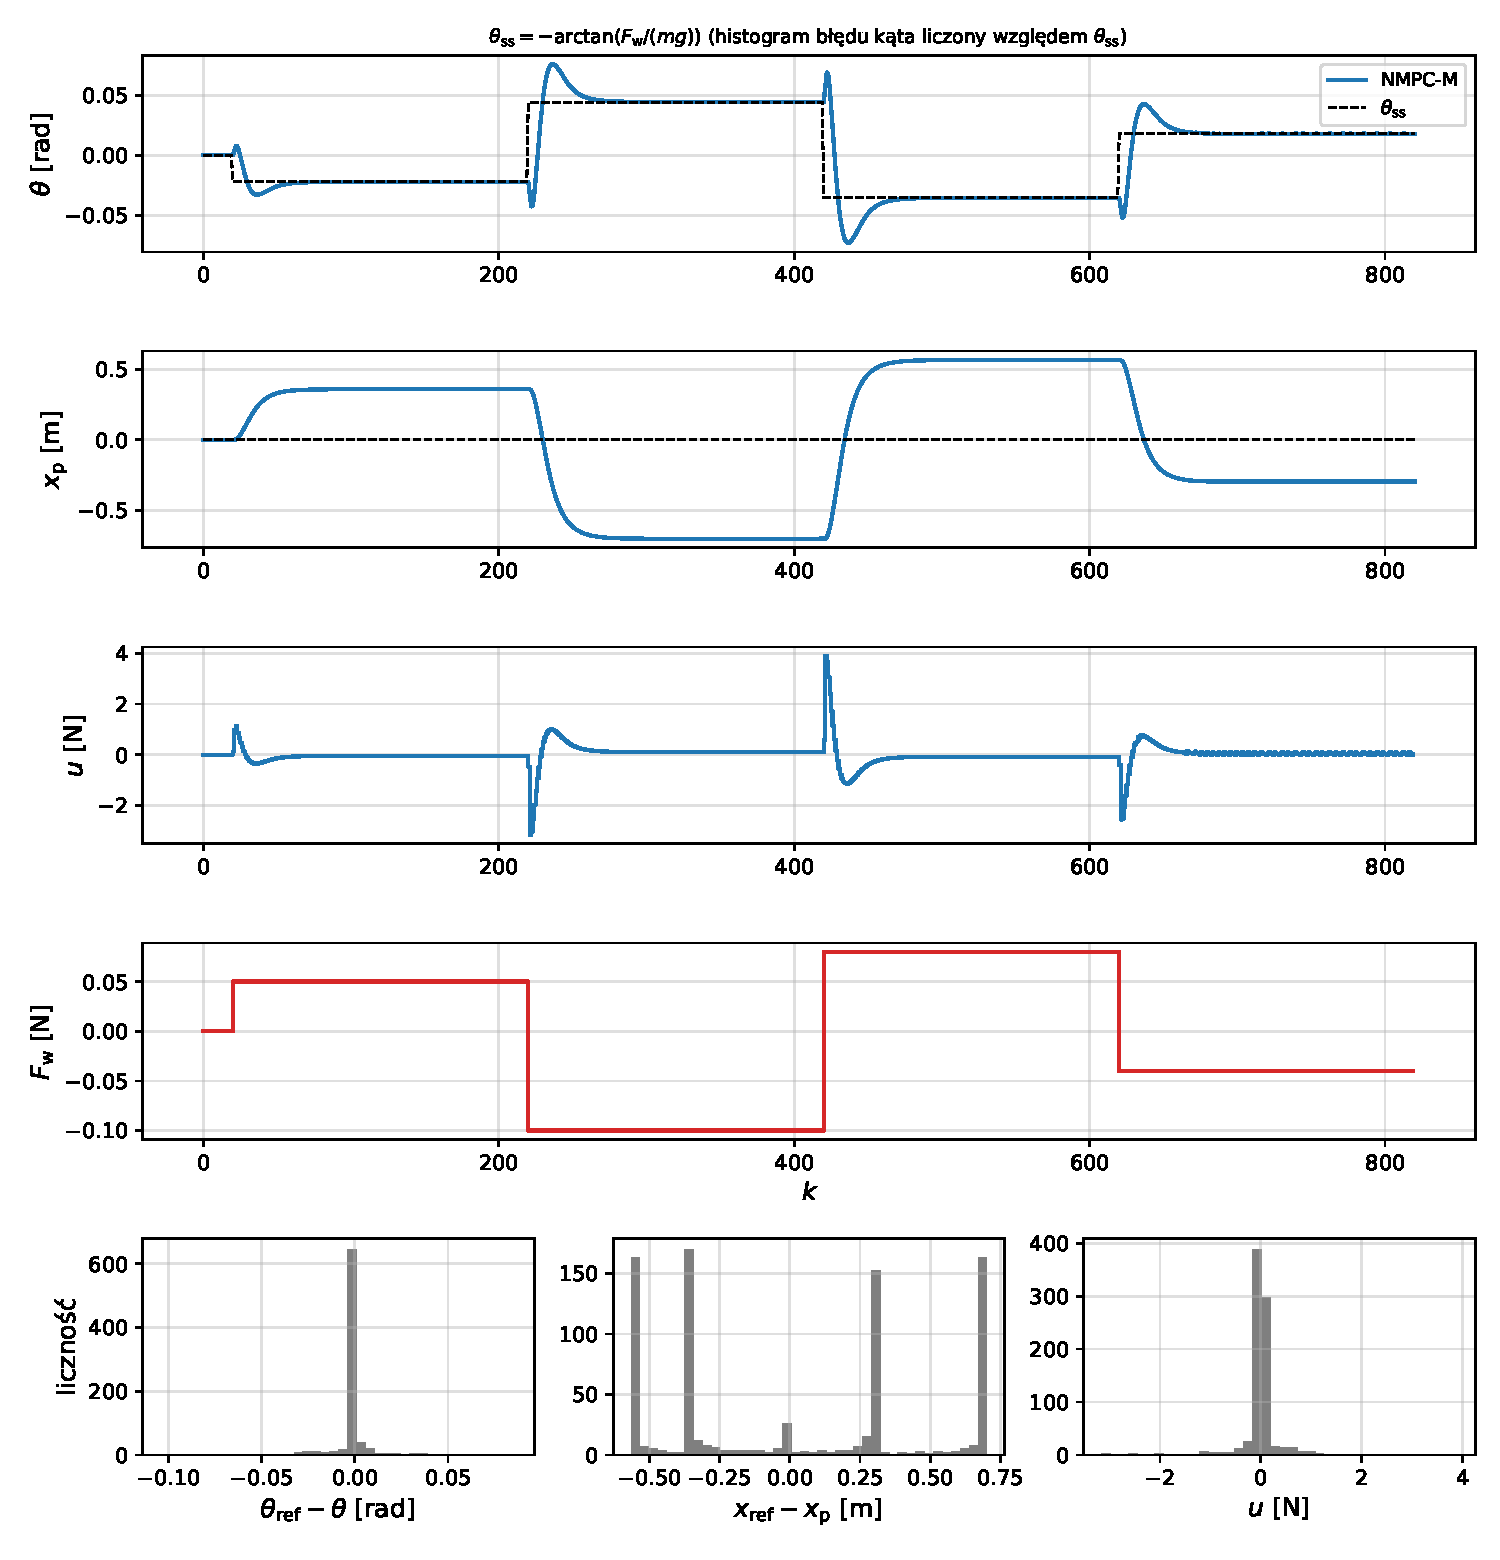
\includegraphics[width=\linewidth]{figs/S2_nmpc_m.pdf}
\caption{NMPC-M, Scenariusz S2 (skoki zakłócenia): status automatyczny -- stabilny.}
\end{figure}
\clearpage
\begin{figure}[p]\centering
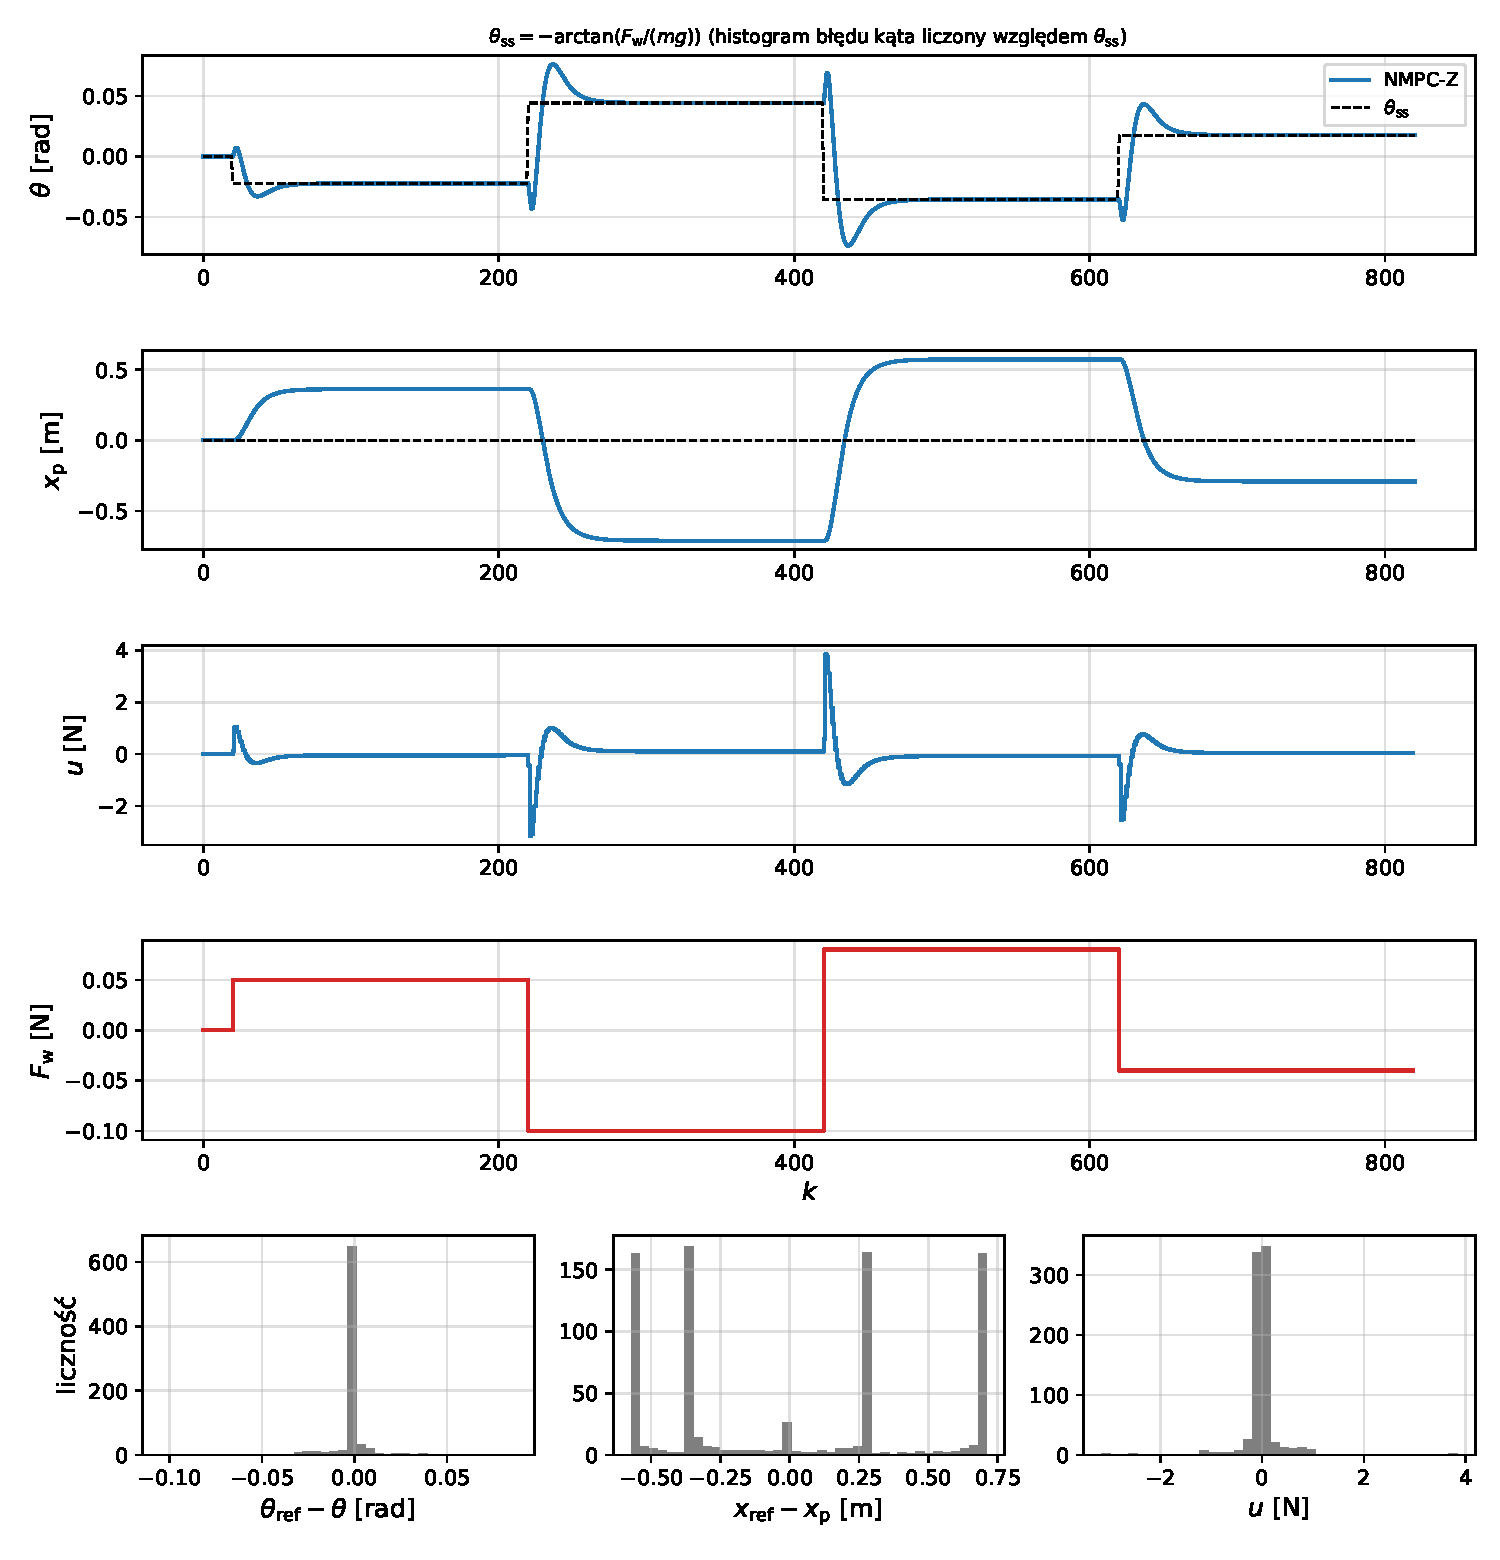
\includegraphics[width=\linewidth]{figs/S2_nmpc_z.pdf}
\caption{NMPC-Z, Scenariusz S2 (skoki zakłócenia): status automatyczny -- stabilny.}
\end{figure}
\clearpage
\begin{figure}[p]\centering
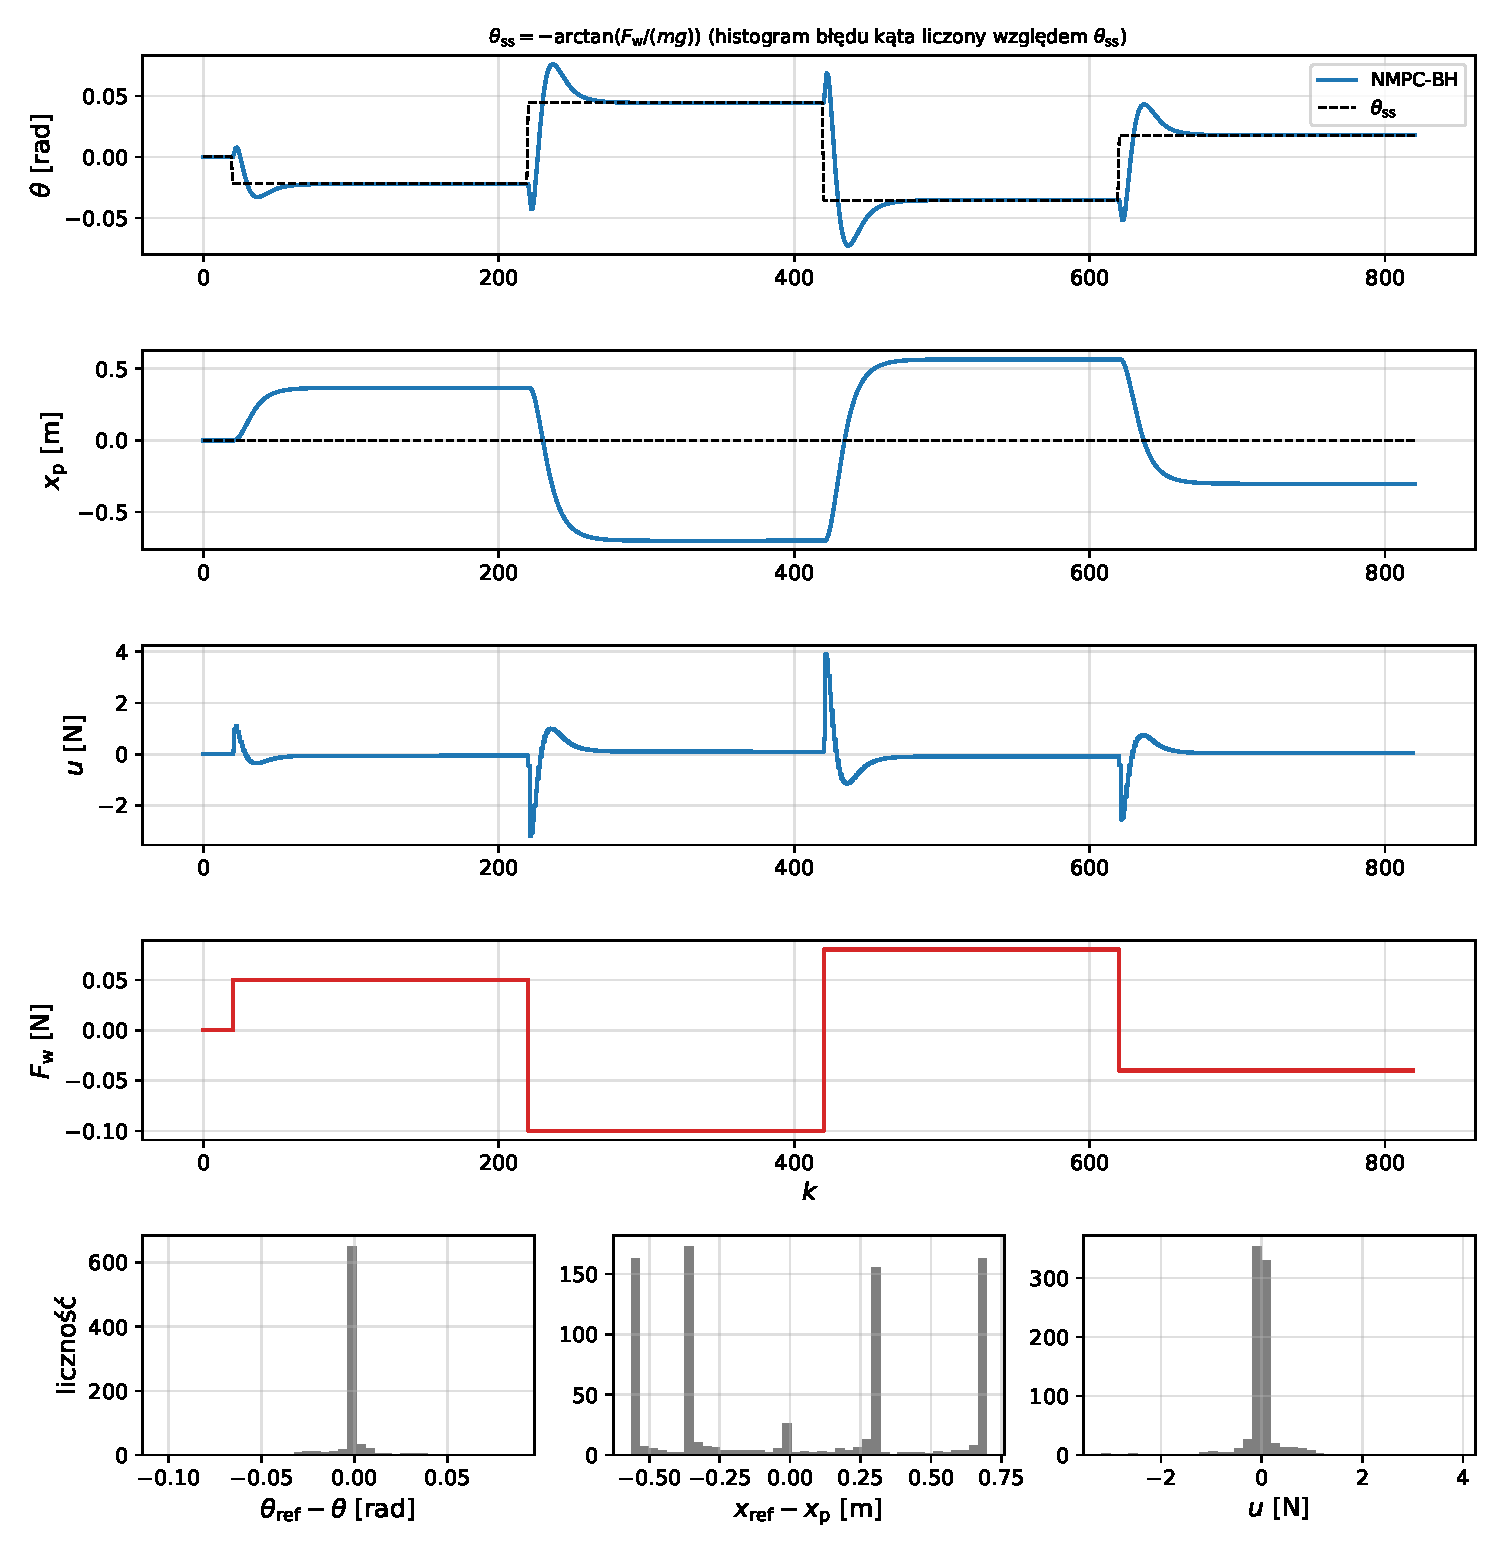
\includegraphics[width=\linewidth]{figs/S2_nmpc_bh.pdf}
\caption{NMPC-BH, Scenariusz S2 (skoki zakłócenia): status automatyczny -- stabilny.}
\end{figure}
\clearpage
\begin{figure}[p]\centering
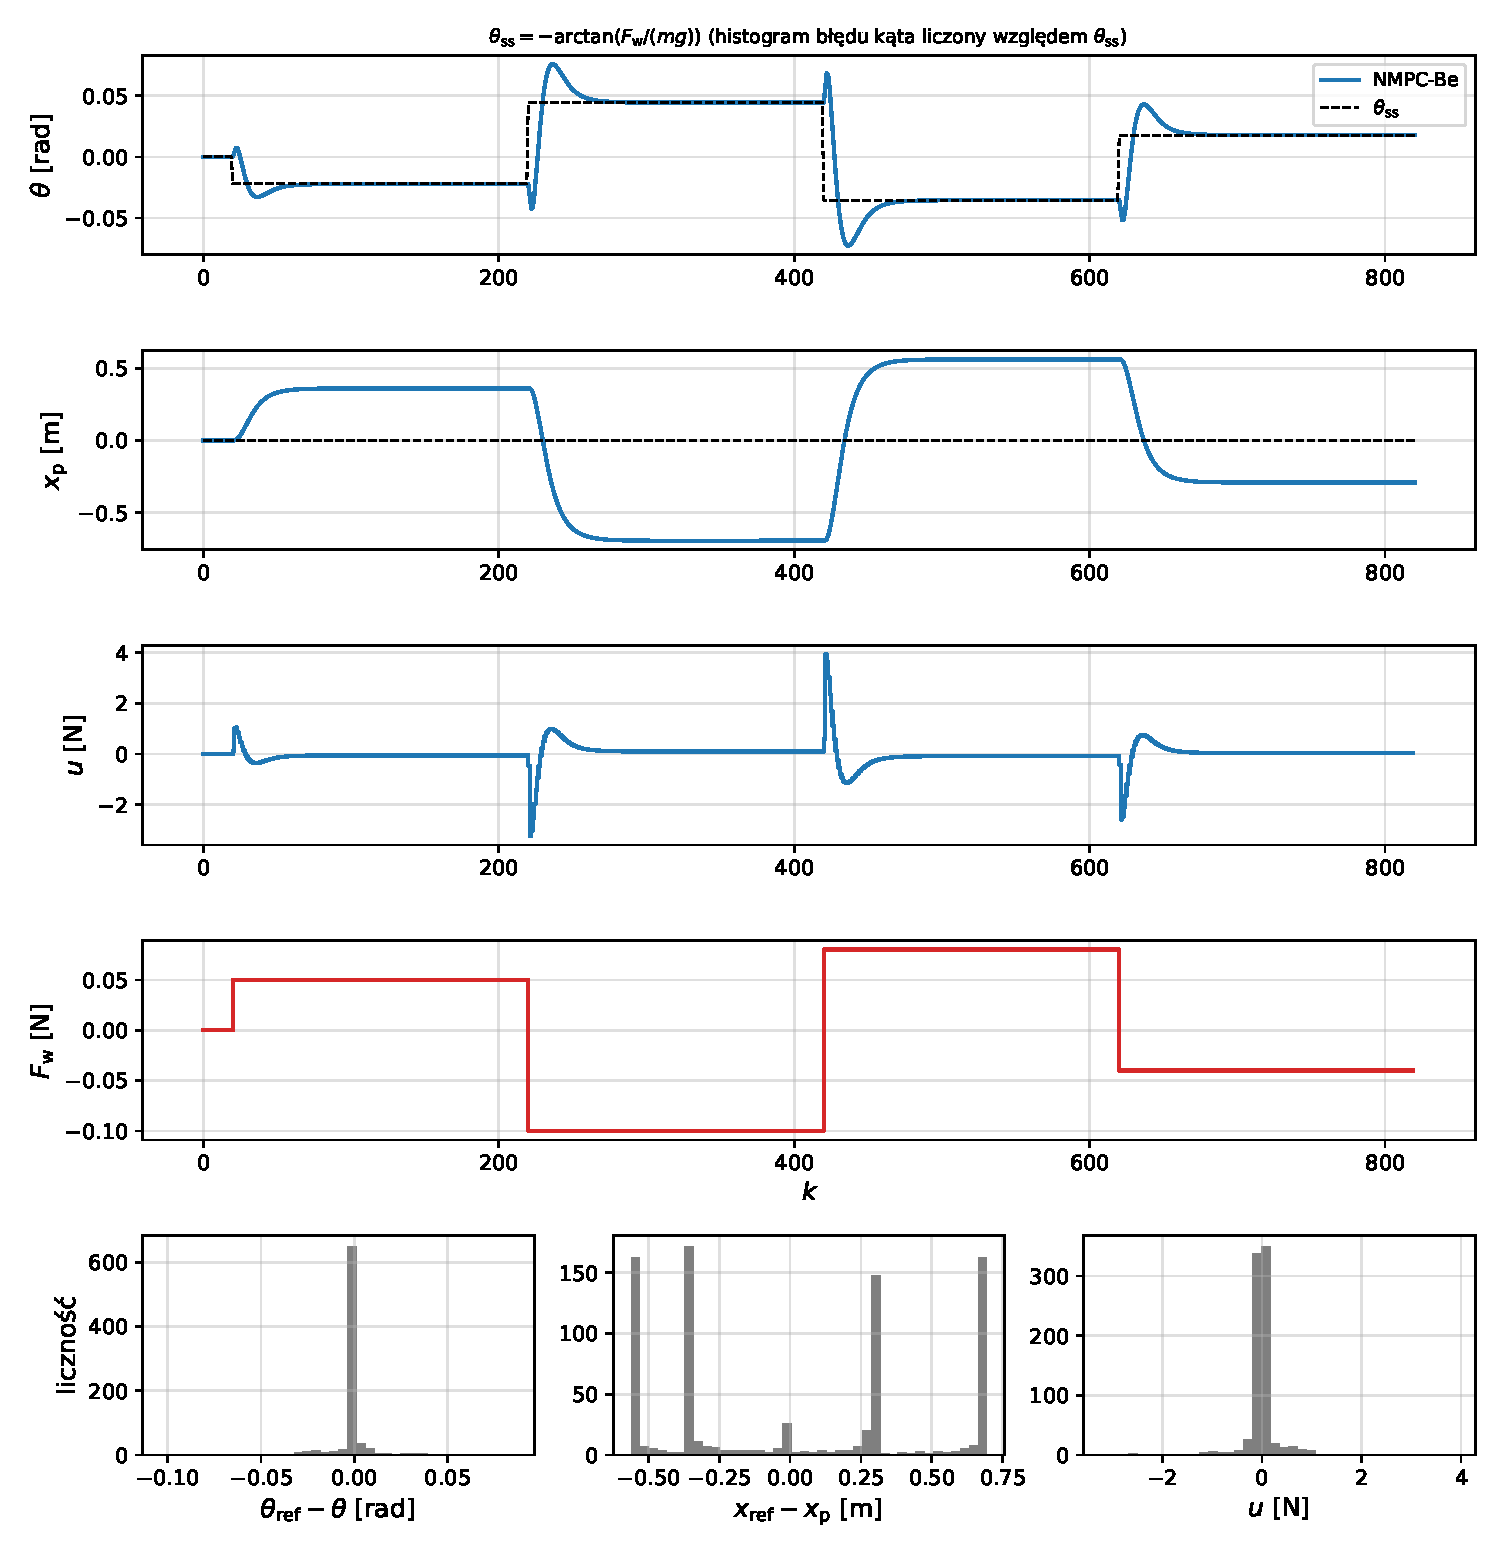
\includegraphics[width=\linewidth]{figs/S2_nmpc_be.pdf}
\caption{NMPC-Be, Scenariusz S2 (skoki zakłócenia): status automatyczny -- stabilny.}
\end{figure}
\clearpage
\begin{figure}[p]\centering
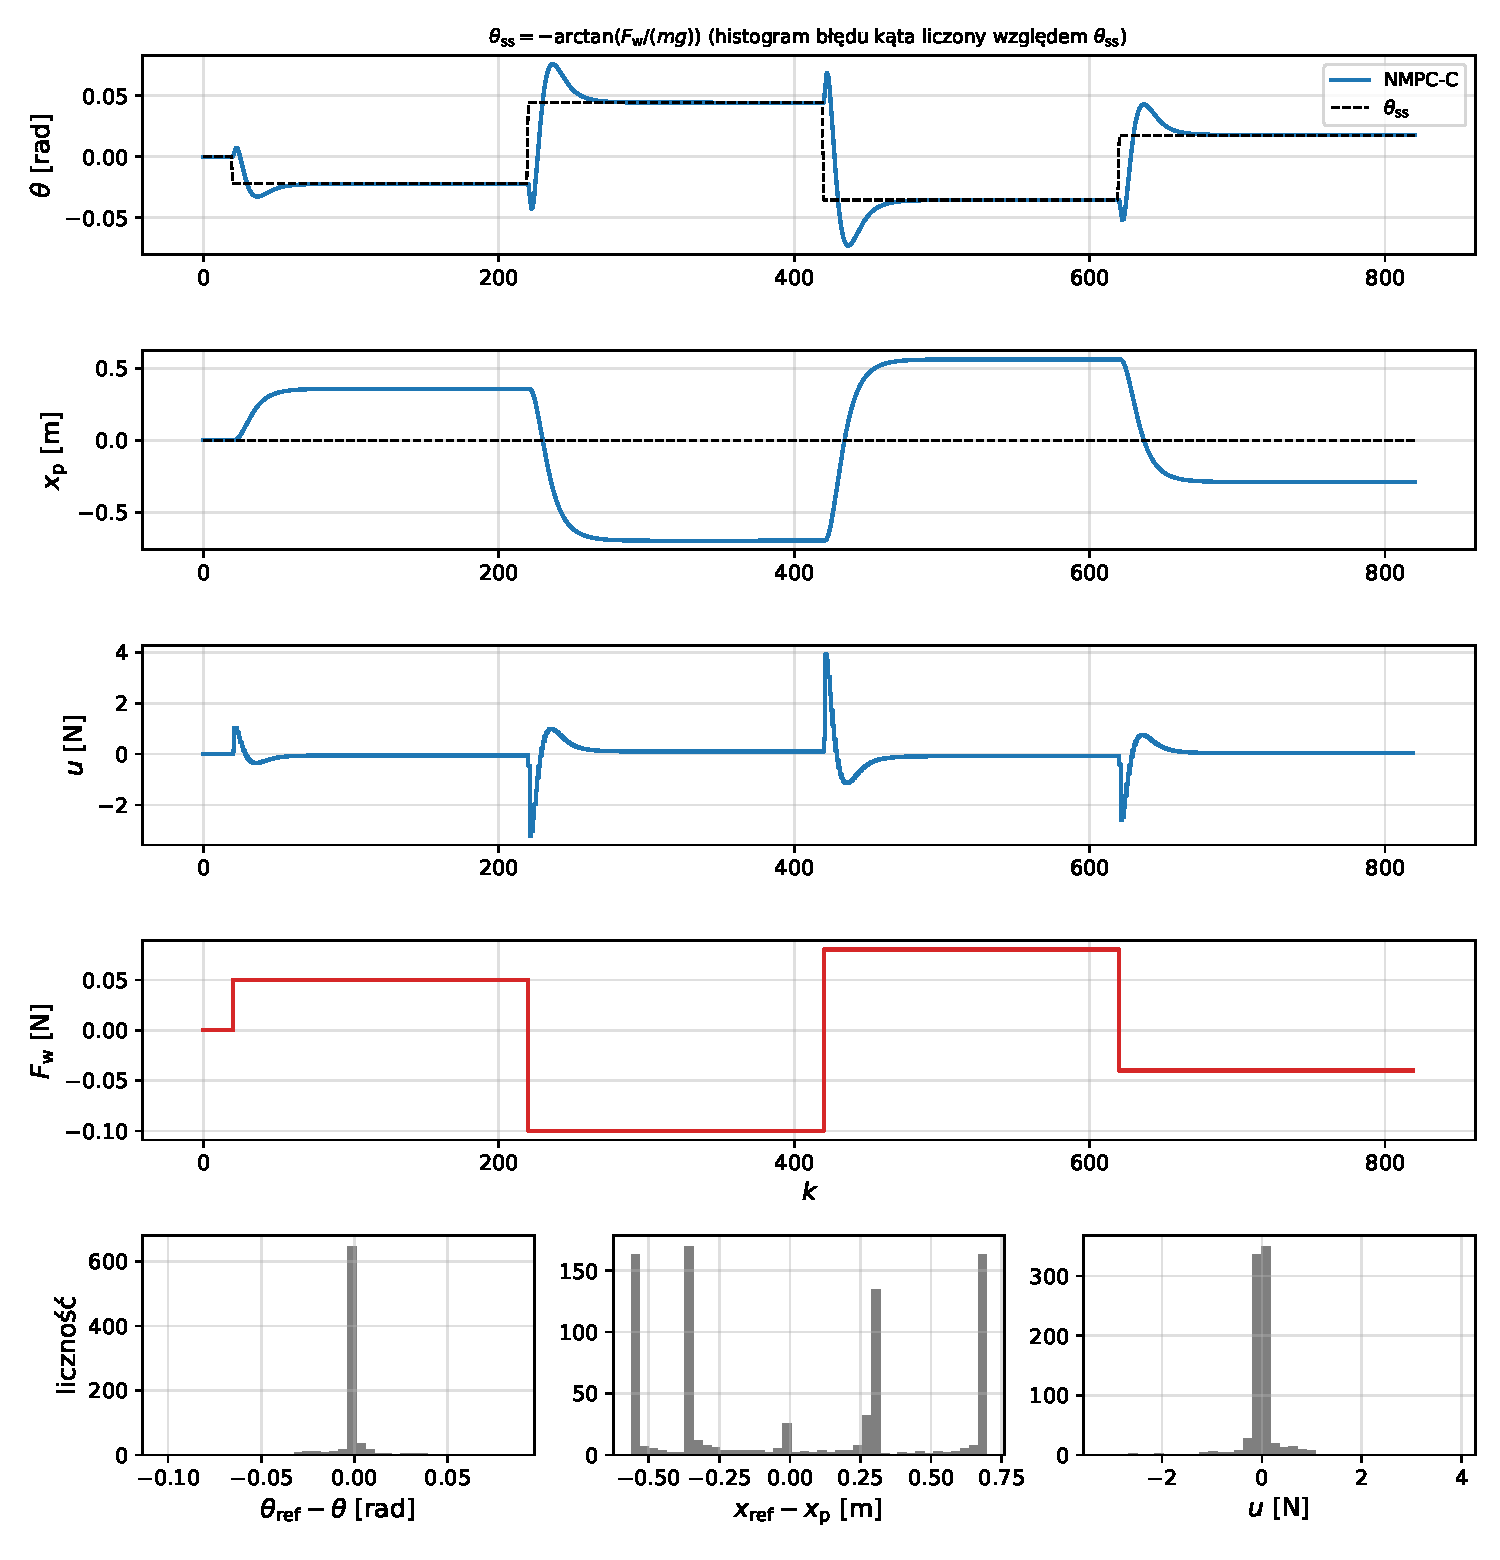
\includegraphics[width=\linewidth]{figs/S2_nmpc_c.pdf}
\caption{NMPC-C, Scenariusz S2 (skoki zakłócenia): status automatyczny -- stabilny.}
\end{figure}
\clearpage
\begin{figure}[p]\centering
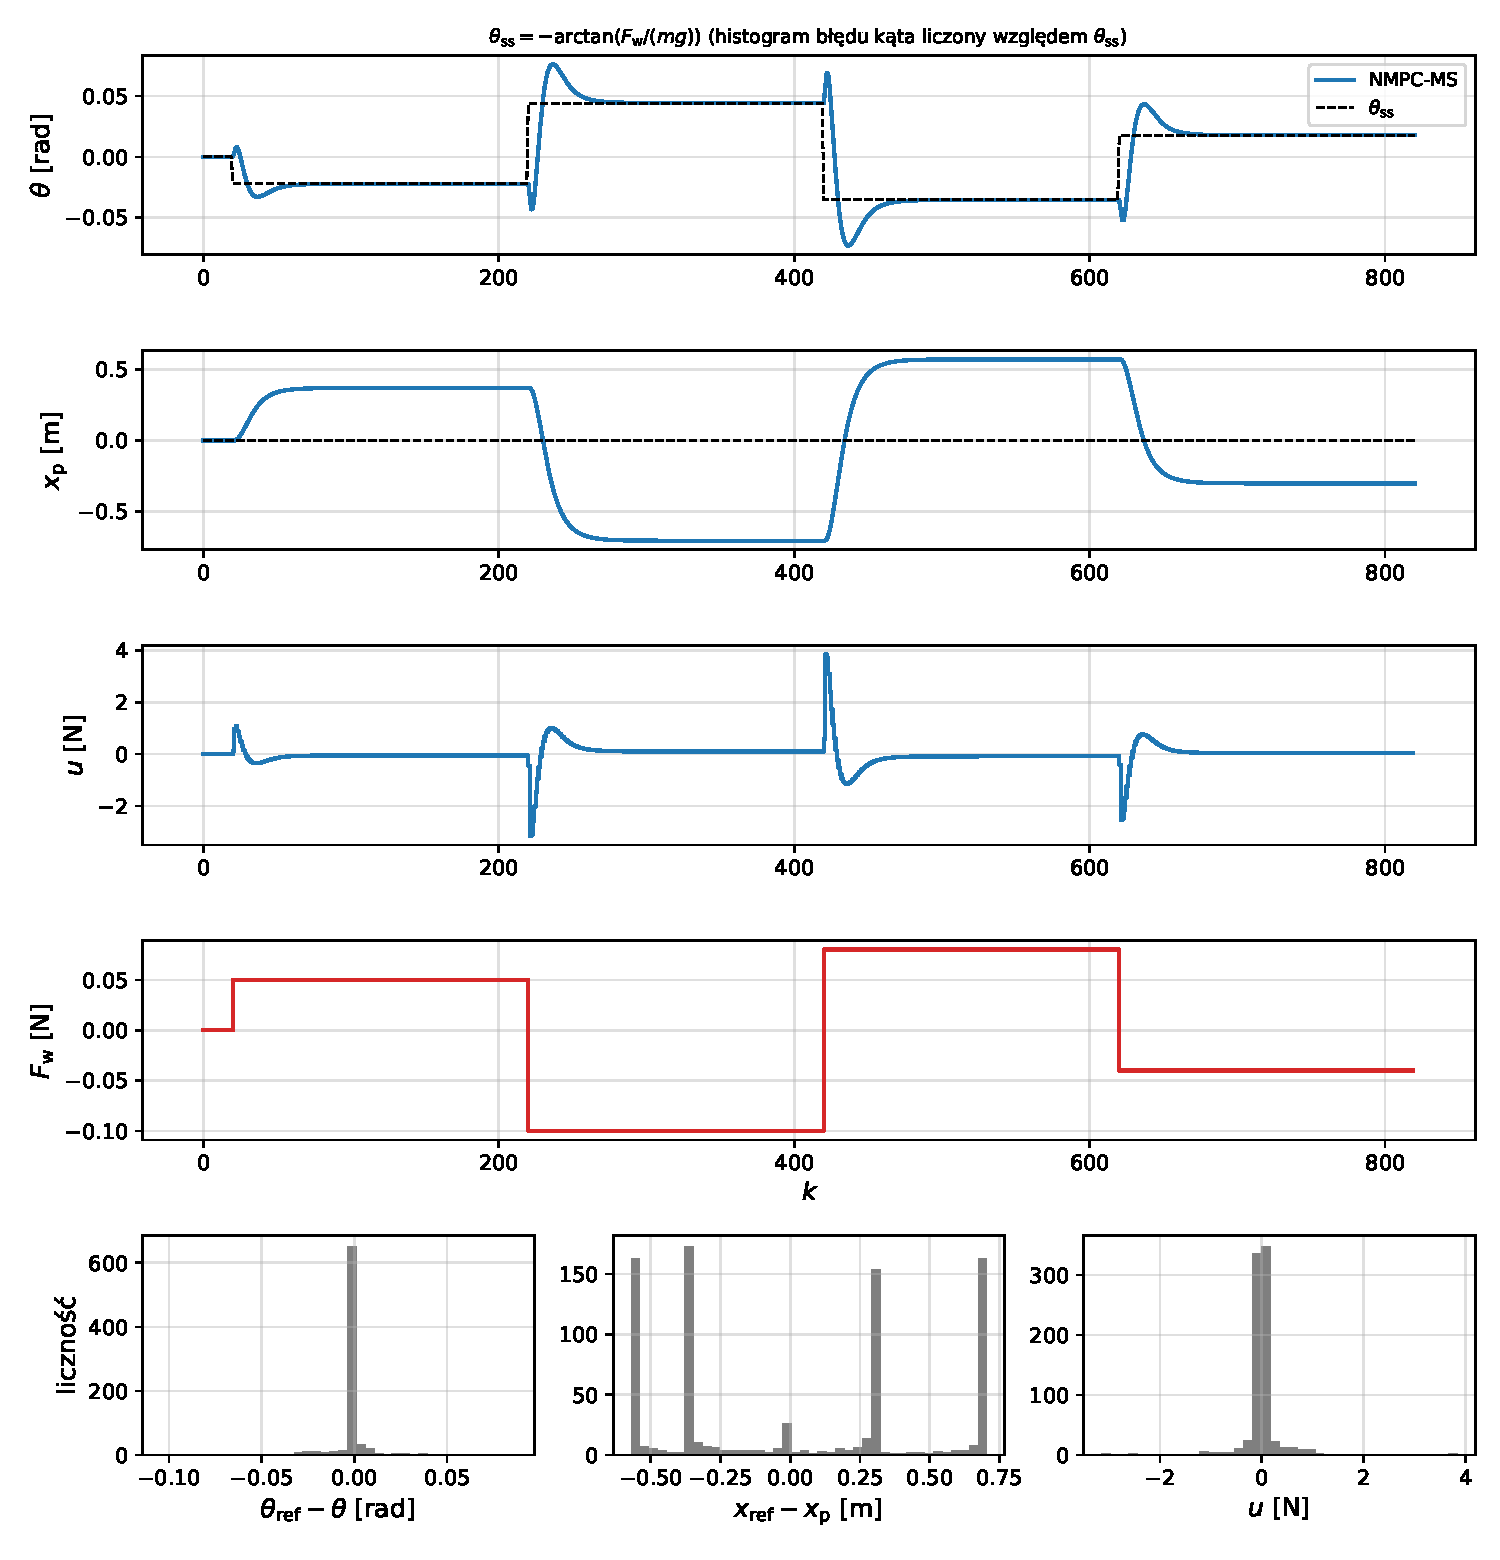
\includegraphics[width=\linewidth]{figs/S2_nmpc_ms.pdf}
\caption{NMPC-MS, Scenariusz S2 (skoki zakłócenia): status automatyczny -- stabilny.}
\end{figure}
\clearpage
\begin{figure}[p]\centering
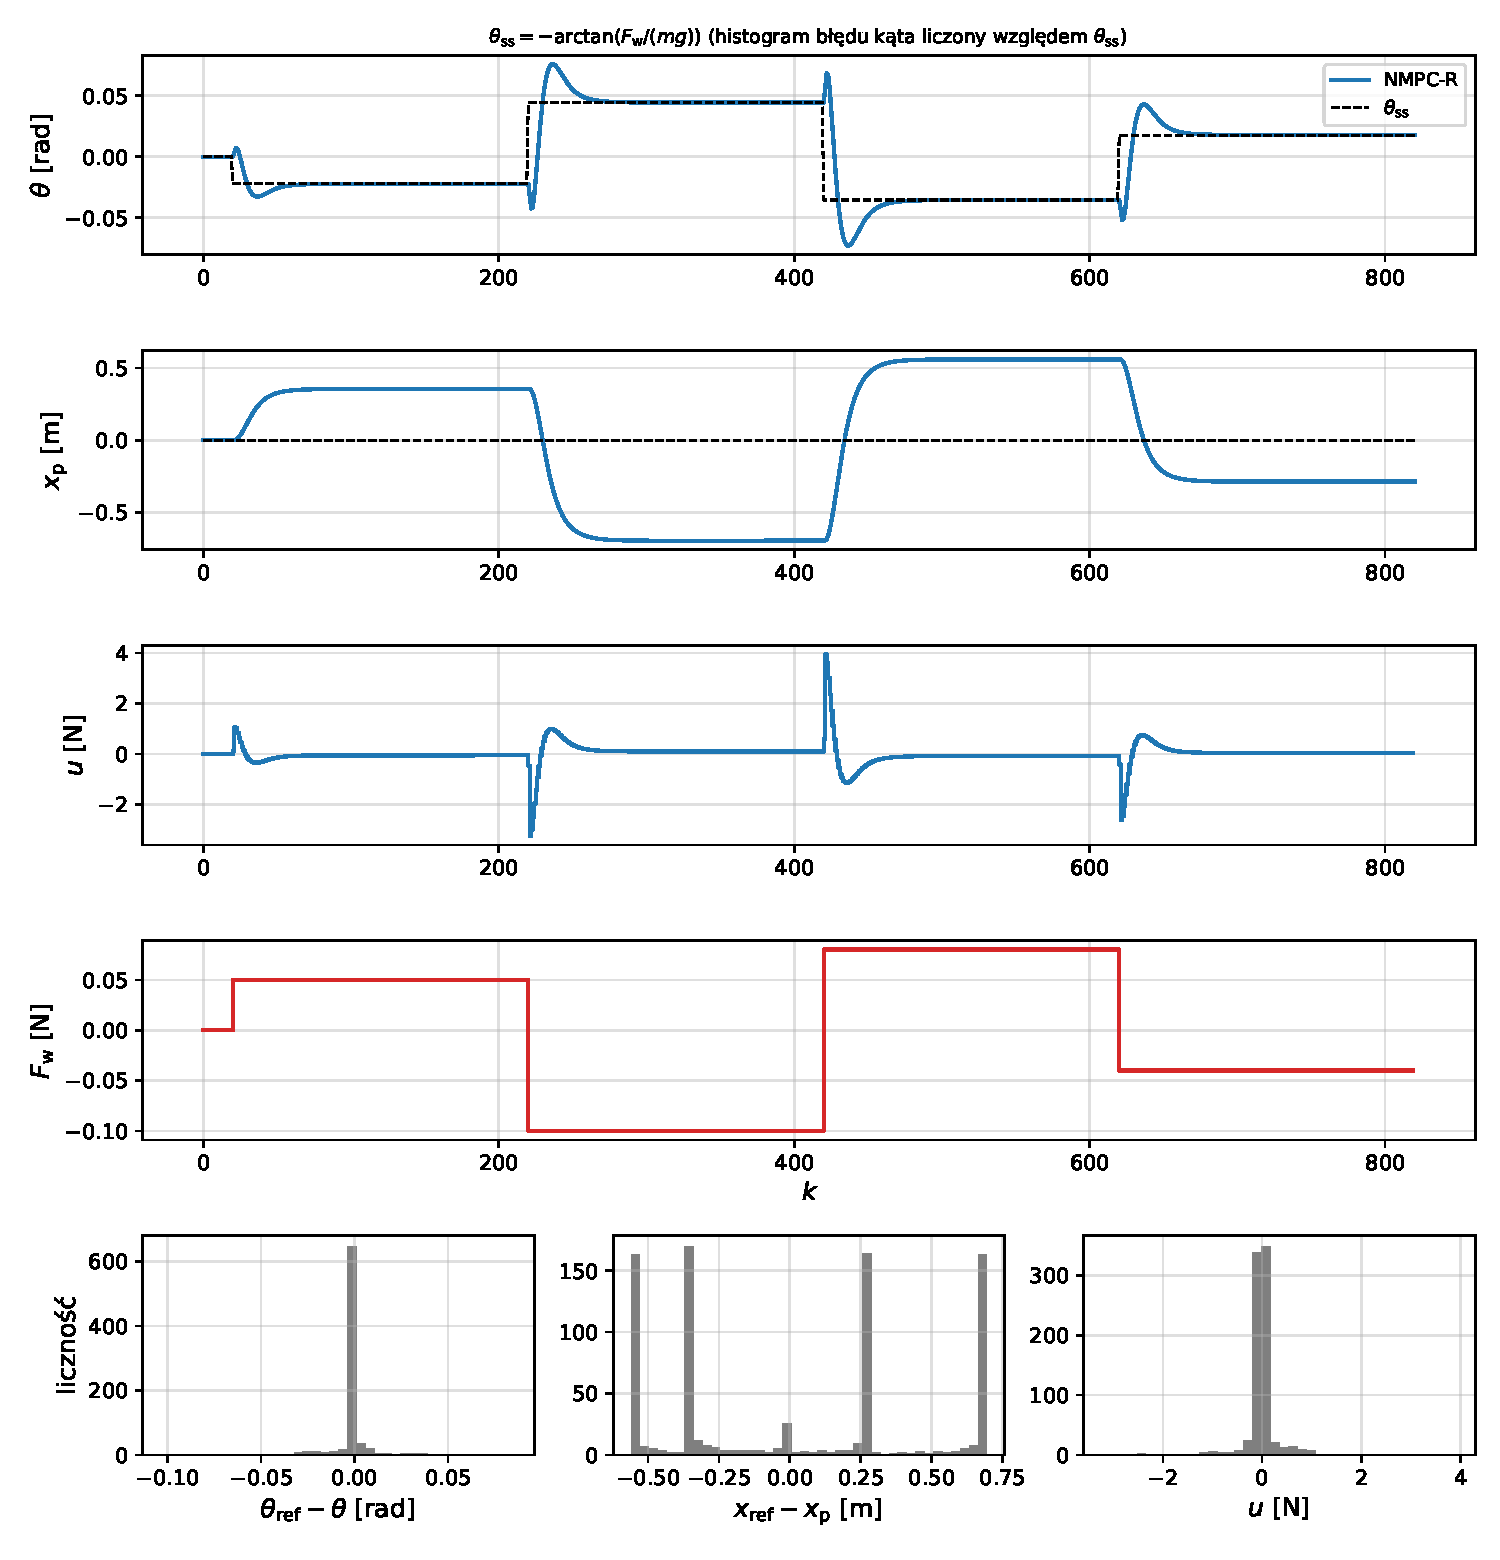
\includegraphics[width=\linewidth]{figs/S2_nmpc_r.pdf}
\caption{NMPC-R, Scenariusz S2 (skoki zakłócenia): status automatyczny -- stabilny.}
\end{figure}
\clearpage
\begin{figure}[p]\centering
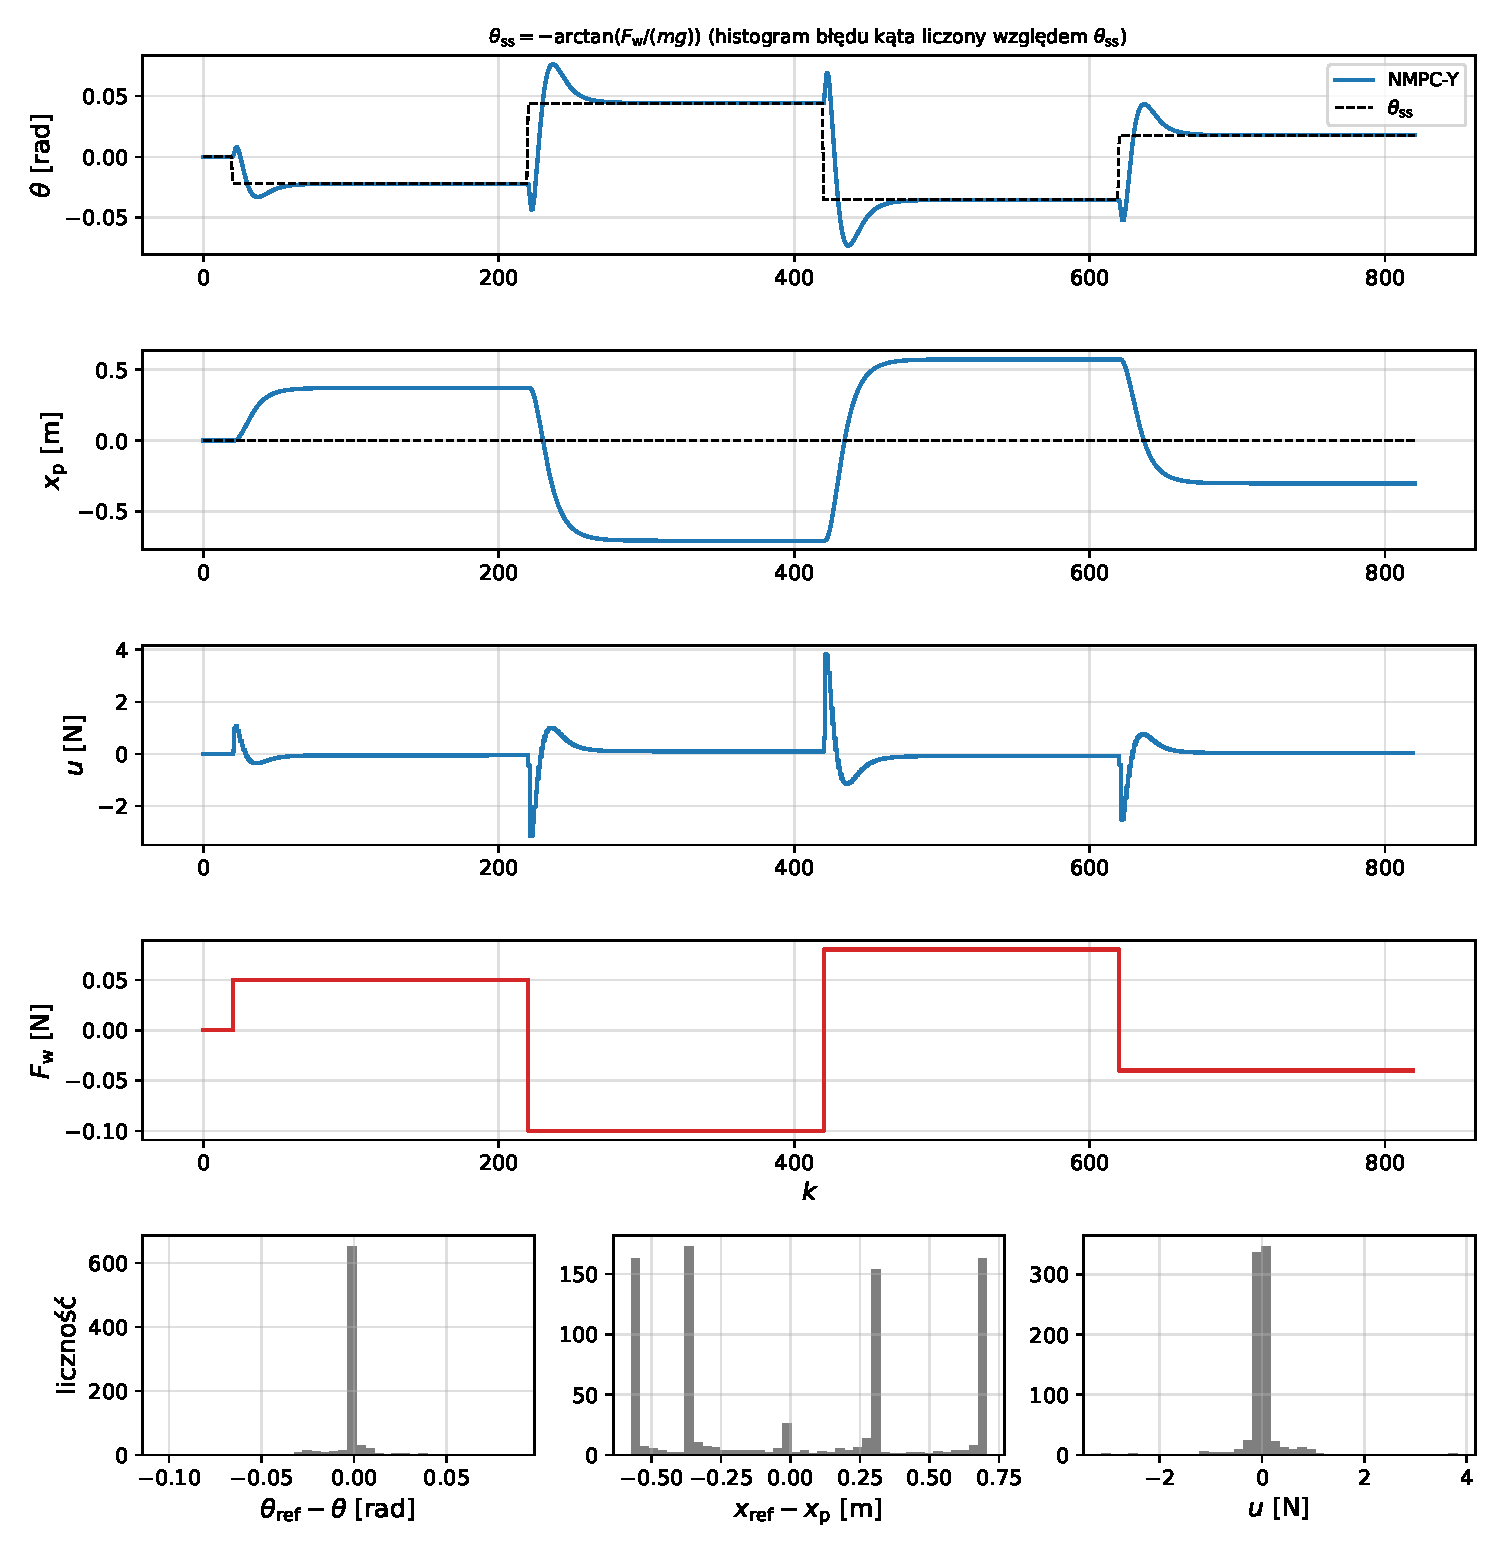
\includegraphics[width=\linewidth]{figs/S2_nmpc_y.pdf}
\caption{NMPC-Y, Scenariusz S2 (skoki zakłócenia): status automatyczny -- stabilny.}
\end{figure}
\clearpage
